%%%%%%
%%%%%%%%%%%%%%%%%%%%%%%%%%%%%% Title Page Info %%%%%%%%%%%%%%%%%%%%%%%%%%%%%%%%%%%%%%%%%%%
%%%%%%%%%%%%%%%%%%%%%%%%%%%%%%%%%%%%%%%%%%%%%%%%%%%%%%%%%%%%%%%%%%%%%%%%%%%%%%%%%%%%%%%%%%

\documentclass[aspectratio=169,compress]{beamer}
\mode<presentation> 

\usetheme{Warsaw}
\usecolortheme[rgb={0.0,0.4,0.4}]{structure}
%\usecolortheme[rgb={0,0.4,0}]{structure}
%\usetheme{AnnArbor}

% define
%\usepackage{beamerouterthememiniframes} % Para los puntitos 
\setbeamertemplate{footline}[frame number]{}

% include packages
\usepackage{subfigure}
\usepackage{multicol}
\usepackage{amsmath}
\usepackage{epsfig}
\usepackage{graphicx}
\usepackage[all,knot]{xy}
\usepackage{algorithmic}
\xyoption{arc}
\usepackage{url}
\usepackage{multimedia}
\usepackage{hyperref}

\usepackage{pgfpages}
\setbeameroption{hide notes} % Only slides
%\setbeameroption{show only notes} % Only notes
%\setbeameroption{show notes on second screen=right} % Both

\title{Titulo Rinbombante de Cualquier cosa Apatalladoras Que nadie entiende pero suenta bien chido..}
%\subtitle{The Beamer Class}
\author{Dr. Marco Aurelio Nu\~no Maganda}
\institute{Universidad Politécnica de Victoria\\ Laboratorio de Sistemas Inteligentes \\
mnunom@upv.edu.mx  \vspace{.25cm} }

\date{Marzo 24, 2022}
%\textbf{nmaganda@ccc.inaoep.mx}

%%%%%%%%%%%%%%%%%%%%%%%%%%%%%%%%%%%%%%%%%%%%%%%%%%%%%%%%%%%%%%%%%%%%%%%%%%%%%%%%%%%%%%%%%%
%%%%%%%%%%%%%%%%%%%%%%%%%%%%%% Begin Your Document %%%%%%%%%%%%%%%%%%%%%%%%%%%%%%%%%%%%%%%
%%%%%%%%%%%%%%%%%%%%%%%%%%%%%%%%%%%%%%%%%%%%%%%%%%%%%%%%%%%%%%%%%%%%%%%%%%%%%%%%%%%%%%%%%%

 

\usepackage[backend=biber,maxcitenames=50,maxbibnames=50,sorting=ydmdddnt]{biblatex}

\DeclareSortingScheme{ydmdddnt}{ 
  \sort{ 
    \field{presort} 
  } 
  \sort[final]{ 
    \field{sortkey} 
  } 
  \sort[direction=descending]{ 
    \field{year} 
  } 
  \sort[direction=descending]{ 
    \field{month} 
  } 
  \sort[direction=descending]{ 
    \field{day} 
  } 
  \sort{ 
    \field{journaltitle} 
  } 
  \sort{ 
    \field{author} 
    \field{editor} 
  } 
  \sort{ 
    \field{title} 
  } 
}




%\renewrobustcmd{\mkbibfootnote}{\normalsize\footnotemark\footnotetext}
\setbeamerfont{footnote}{size=\tiny}






\newcommand{\ArchivoPrincipal}{Todos}
\newcommand{\ArchivoSecundario}{Bibliografia}


%Append keywords to identify different bibliography entries.
\DeclareSourcemap{
  \maps[datatype=bibtex, overwrite]{
    \map{
      \perdatasource{\ArchivoPrincipal.bib}
      \step[fieldset=KEYWORDS, fieldvalue=primary, append]
    }
    \map{
      \perdatasource{\ArchivoSecundario.bib}
      \step[fieldset=KEYWORDS, fieldvalue=secundary, append]
    }    
  }
}


\addbibresource{\ArchivoPrincipal.bib}
\addbibresource{\ArchivoSecundario.bib}

\usepackage{listings}
 
 \AtBeginSection[]
{
    \begin{frame}
        \frametitle{Outline}
        \tableofcontents[currentsection]
    \end{frame}
}



\begin{document}

\frame{
	%\titlepage 
	\begin{titlepage}
	\end{titlepage}
	
}

\frame{
\frametitle{Contenido}
\tableofcontents
}

% Parte V: Desarrollos Tecnologicos (No publicados formalmente)
\section{Proyectos Estudiantiles y en Desarollo}


\begin{frame}{Recorrido UPV Virtual en teléfonos inteligentes}
%\begin{block}{Recorrido UPV Virtual en teléfonos inteligentes} 
Demo incremental, que emplea OpenGL ES 2.0 (compatible con el 100\% de los smartphones). 
\begin{itemize}
\item Versión 1: Solo mundo virtual (no inmersivo). El usuario se movía con presionando teclas de la interfaz de usuario
\item Versión 2: Mundo virtual inmersivo (integrado a unos lentes). El usuario movía la vista mediante los datos obtenidos por el sensor giroscopio del teléfono inteligente y avanzaba usando un manos libres alámbrico.
\item Versión 3: Controlado por voz. El usuario se movía dentro del entorno mediante comandos de voz.
\item Versión 3.5: Controlado mediante control de videojuegos (Bluetooth o USB)
\end{itemize}
%\end{block} 
\end{frame}

\renewcommand{\EntradaBibtex}{Reporte2019}
\begin{frame}{\citetitle{\EntradaBibtex} \footnotemark[1] (1)}

%\begin{frame}{Recorrido UPV Virtual 1.0\footnotemark }
%\begin{block}{} 
\begin{columns}
\begin{column}{0.48\textwidth}
    \begin{center}

\begin{itemize}
\item La navegación es mediante botones (adelante, atrás, izquierda, derecha, subir, bajar)
\item Una potencial mejora es mediante eventos de toque en pantalla
\end{itemize}
     \end{center}

\end{column}
\begin{column}{0.52\textwidth}  
    \begin{center}
\begin{itemize}
\end{itemize}
     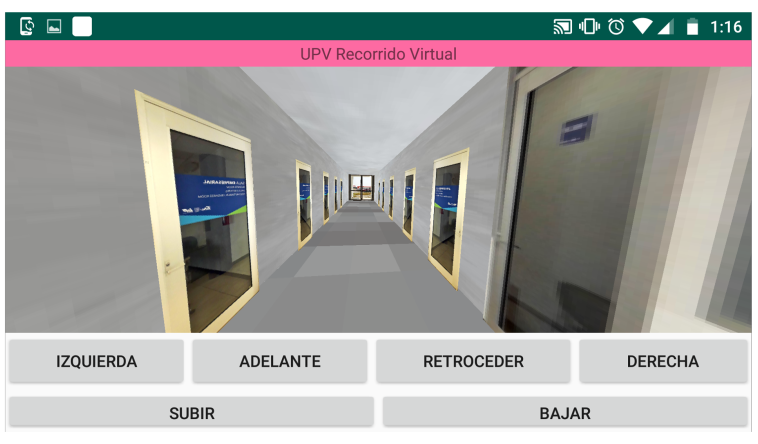
\includegraphics[width=0.9\textwidth]{Figs/RecorridoUPV_V1}\\
     \end{center}
\end{column}
\end{columns}
%\end{block} 
\footnotetext[1]{\fullcite{\EntradaBibtex}}
%\footnotetext{Baez Zapata Marıa Fernanda, Cárdenas Castillo Jesús Alfredo, Olvera Osuna José Armando and Wang Yu Hsiang. \textbf{Recorrido UPV en Android}. Proyecto Final de la Asignatura ``Cómputo en Dispositivos Móviles'', 2019. Sin Publicar.}
%\\setcounter{footnote}{0}
\end{frame}


%\begin{frame}{Recorrido UPV Virtual 1.0 (2)}
%\renewcommand{\EntradaBibtex}{Reporte2019}
\begin{frame}{\citetitle{\EntradaBibtex}  (2)}
%\begin{block}{Recorrido UPV Virtual 1.0 (2)} 
\begin{itemize}
\item Vistas de los diferentes edificios
\end{itemize}
    \begin{center}
     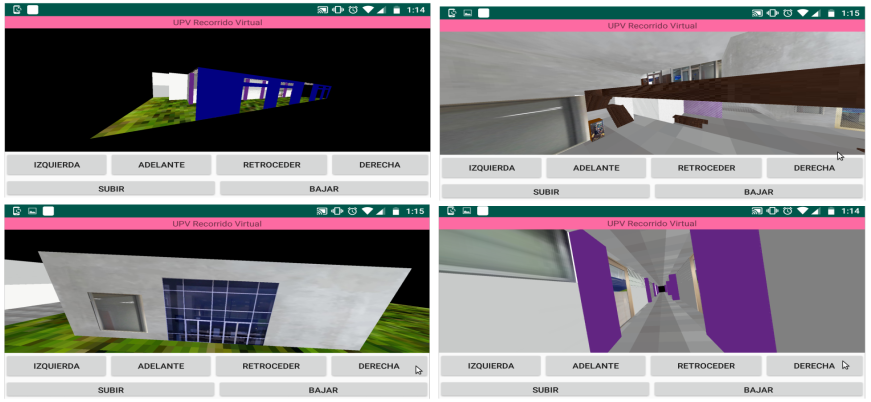
\includegraphics[width=0.80\textwidth]{Figs/RecorridoUPV_V2}\\
     \end{center}
%\end{block} 
\end{frame}

\renewcommand{\EntradaBibtex}{RecorridoVirtualLentesVR_2019}
%\begin{frame}{Recorrido UPV Virtual 2.0\footnotemark}
\begin{frame}{\citetitle{\EntradaBibtex}  (2)}
%\begin{block}{Recorrido UPV Virtual 2.0\footnotemark} 
\begin{columns}
\begin{column}{0.48\textwidth}
    \begin{center}

\begin{itemize}
\item Se extendió el demo 1.0 para generar una vista dual, requerida para su uso en conjunto con un armazón de VR.
\item La vista cambia en base a lo obtenido por el giroscopio, y el movimiento se controla mediante el botón del manos libres.
\end{itemize}
     \end{center}

\end{column}
\begin{column}{0.52\textwidth}  
    \begin{center}
\begin{itemize}
\end{itemize}
     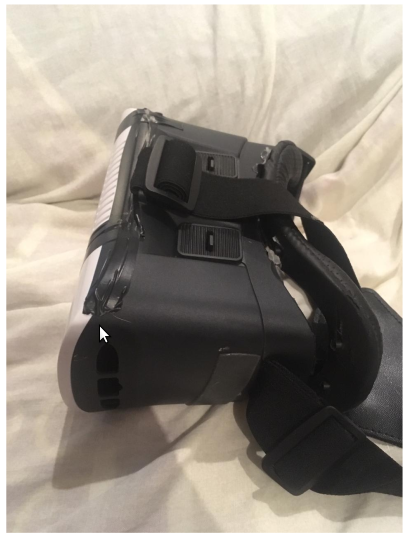
\includegraphics[width=0.4\textwidth]{Figs/RecorridoUPV_V3}\\
     \end{center}
\end{column}
\end{columns}
%\end{block} 
%\footnotetext{\fullcite{RecorridoVirtualLentesVR_2019}}
\footnotetext[1]{\fullcite{\EntradaBibtex}}
%\footnotetext{Alarcon Longoria Carlos Alberto, Alonso Cepeda Leonardo Daniel and Torres Grimaldo Luis Angel. \textbf{Recorrido UPV Virtual en Android}.  Proyecto Final de la Asignatura ``Cómputo en Dispositivos Móviles'', 2019. Sin Publicar.}
%\\setcounter{footnote}{0}
\end{frame}


\renewcommand{\EntradaBibtex}{RecorridoVirtualLentes_ComandosVoz2020}
\begin{frame}{\citetitle{\EntradaBibtex}  (1)}
%\begin{block}{Recorrido UPV Virtual 3.0\footnotemark} 
\begin{columns}
\begin{column}{0.48\textwidth}
    \begin{center}
\begin{itemize}
\item Se eliminó el uso del botón del manos libres para incluir comandos de voz
\item La aplicación respondía a los comandos de voz, de tal forma que el usuario no debería mover nada
\end{itemize}
     \end{center}

\end{column}
\begin{column}{0.52\textwidth}  
    \begin{center}
     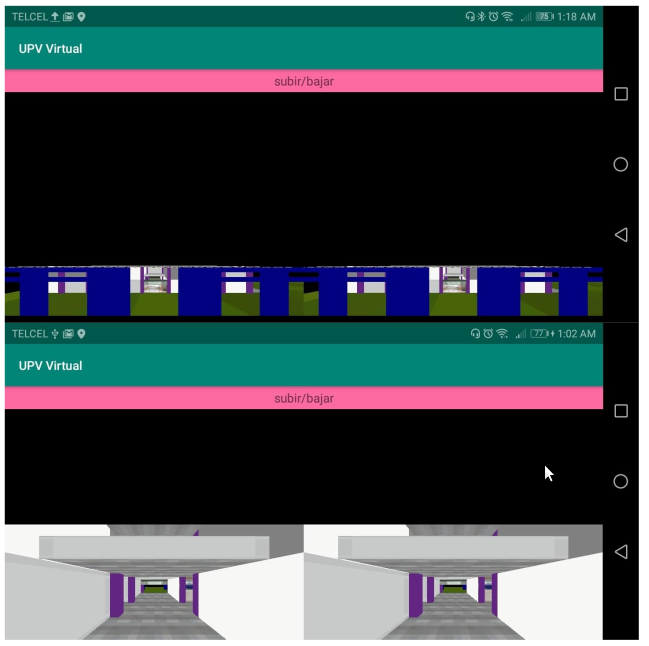
\includegraphics[width=0.6\textwidth]{Figs/RecorridoUPV_V5}\\
     \end{center}
\end{column}
\end{columns}
%\end{block} 
\footnotetext[1]{\fullcite{\EntradaBibtex}}
%\footnotetext{José Treviño Olvera. \textbf{Recorrido UPV Virtual en Android con Controles de Voz.}  Proyecto Final de la Asignatura. ``Cómputo en Dispositivos Móviles'', 2020. Sin Publicar.}
%\\setcounter{footnote}{0}
\end{frame}

\renewcommand{\EntradaBibtex}{RecoridoUPV_controles_2021}
%\begin{frame}{Recorrido UPV Virtual 3.5 \footnotemark}
%\begin{block}{Recorrido UPV Virtual 3.5 \footnotemark } 
\begin{frame}{\citetitle{\EntradaBibtex}  (1)}
\begin{itemize}
\item Se incorporaron varios controles de consolas de videojuego para la navegación.
\end{itemize}
\begin{columns}
\begin{column}{0.48\textwidth}
\begin{center}
	\begin{tabular}{ccc}
		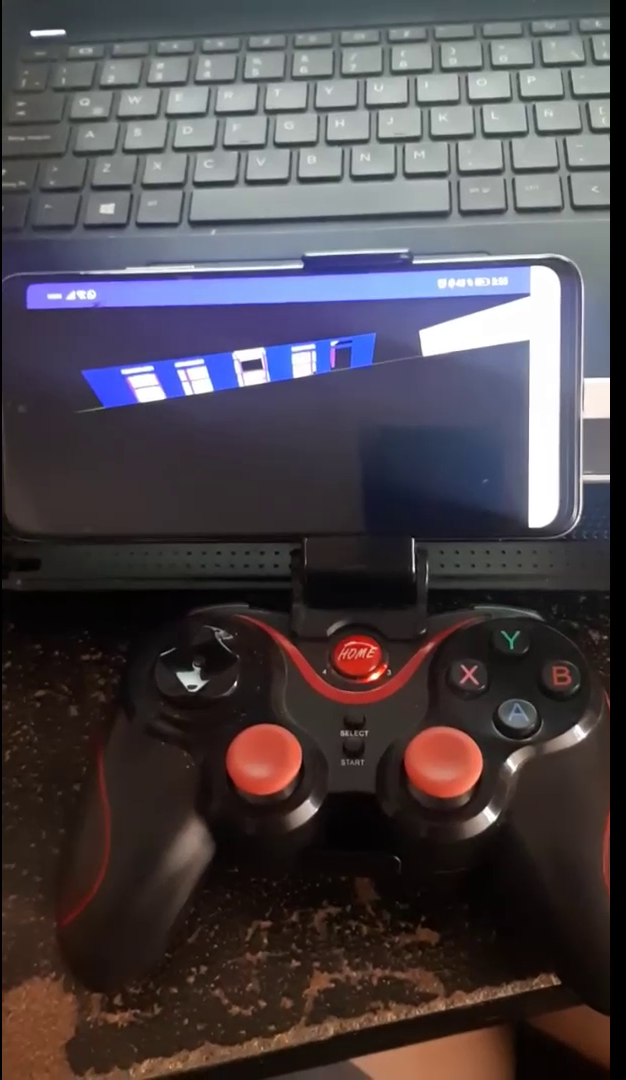
\includegraphics[width=0.25\linewidth]{Figs/UPV_Control01} & 		
		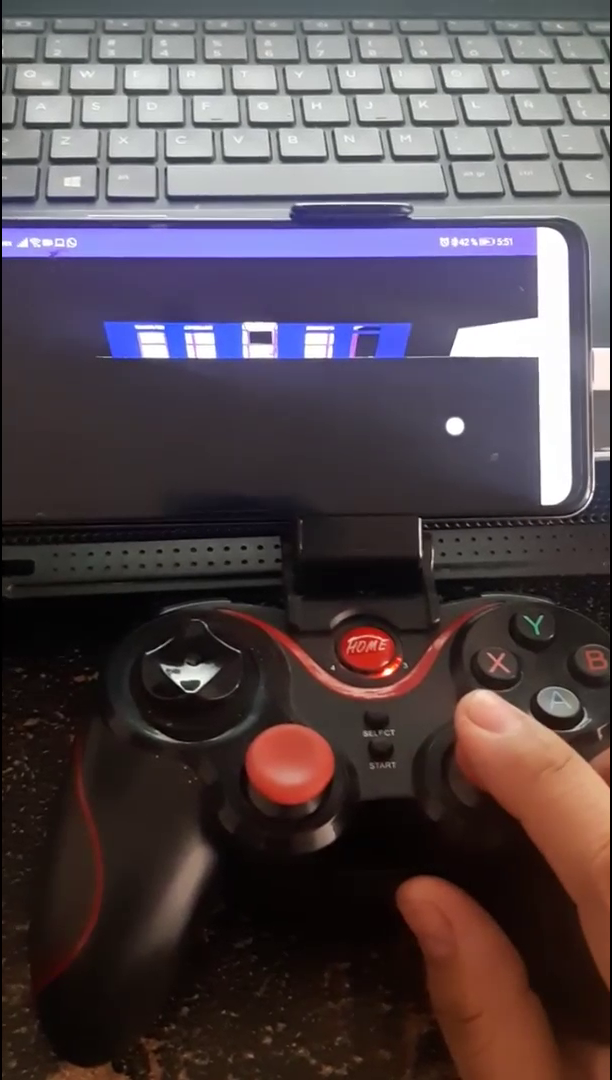
\includegraphics[width=0.25\linewidth]{Figs/UPV_Control02} & 
        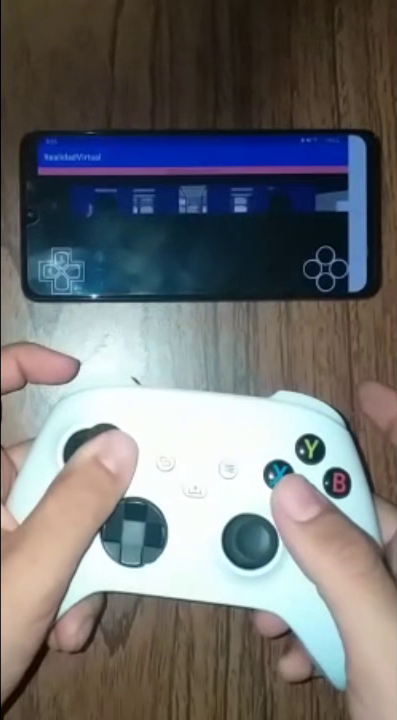
\includegraphics[width=0.25\linewidth]{Figs/UPV_Control04}\\
	\end{tabular}
\end{center}
\end{column}
\begin{column}{0.48\textwidth}
\begin{center}
	\begin{tabular}{c}
		    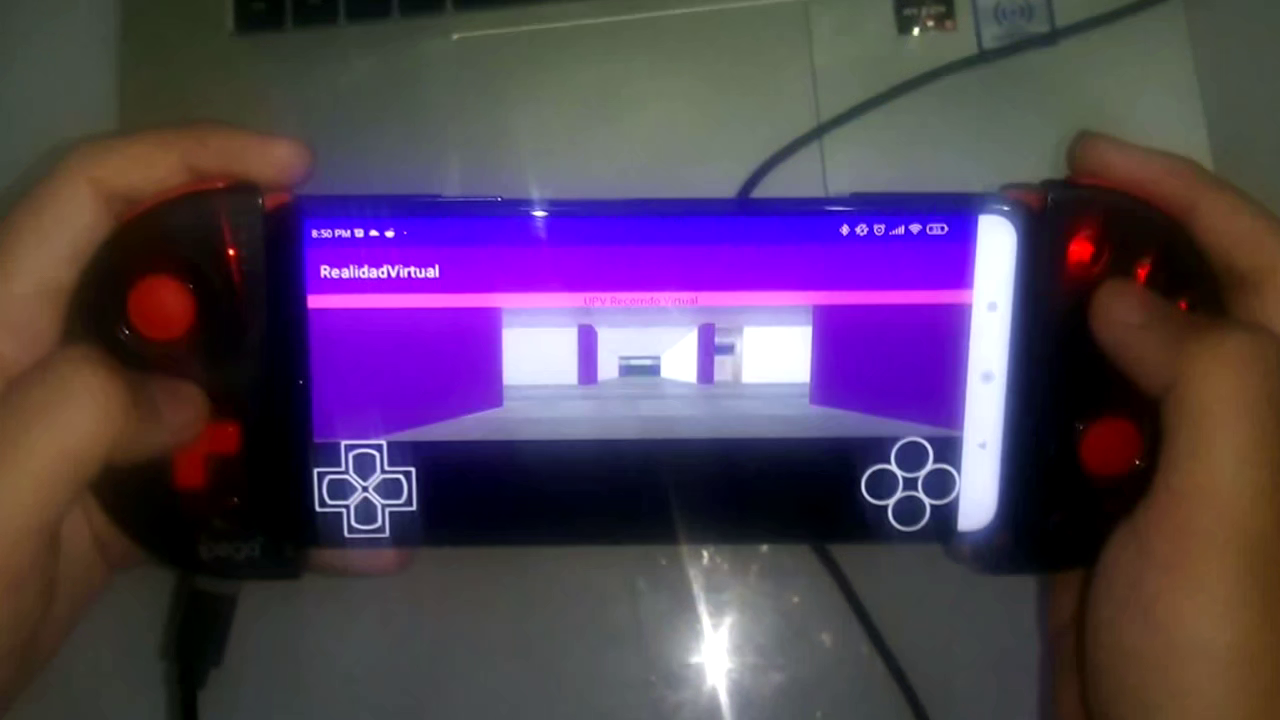
\includegraphics[width=0.45\linewidth]{Figs/UPV_Control03}\\
		    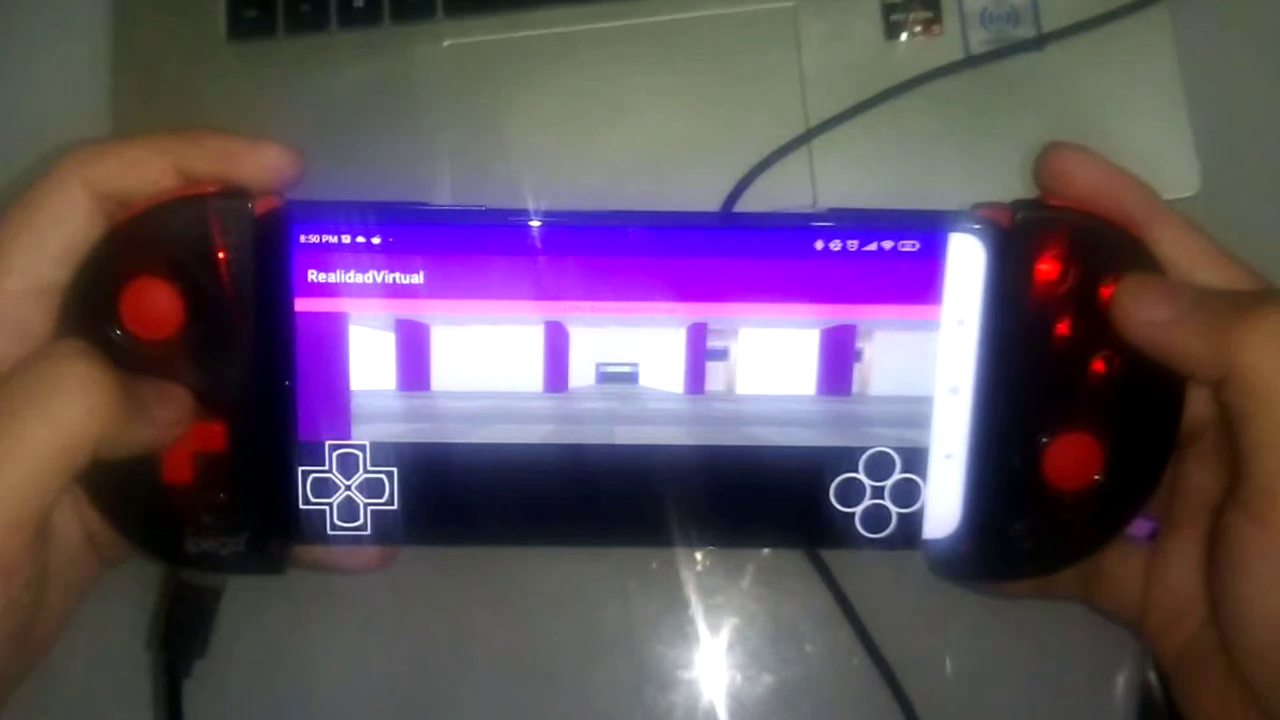
\includegraphics[width=0.45\linewidth]{Figs/UPV_Control05}\\
	\end{tabular}
\end{center}	
\end{column}
\end{columns}
%\end{block} 
\footnotetext[1]{\fullcite{\EntradaBibtex}}
%\footnotetext{\fullcite{RecoridoUPV_controles_2021}}
\end{frame}



\renewcommand{\EntradaBibtex}{BrazoRobot_Morin2019}
\begin{frame}{\citetitle{\EntradaBibtex} \footnotemark[1] (1)}
%\begin{block}{Brazo Robótico \footnotemark} 
\begin{columns}
	\begin{column}{0.55\textwidth}
		\begin{itemize}
			\item Se retoma un diseño previamente realizado para WebGL. 
			\item Los componentes del robot son movidos mediante motores, y puede ser visto desde difentes perspectivas.		
		\end{itemize}
	\end{column}
	\begin{column}{0.22\textwidth}
		 \begin{center}
		     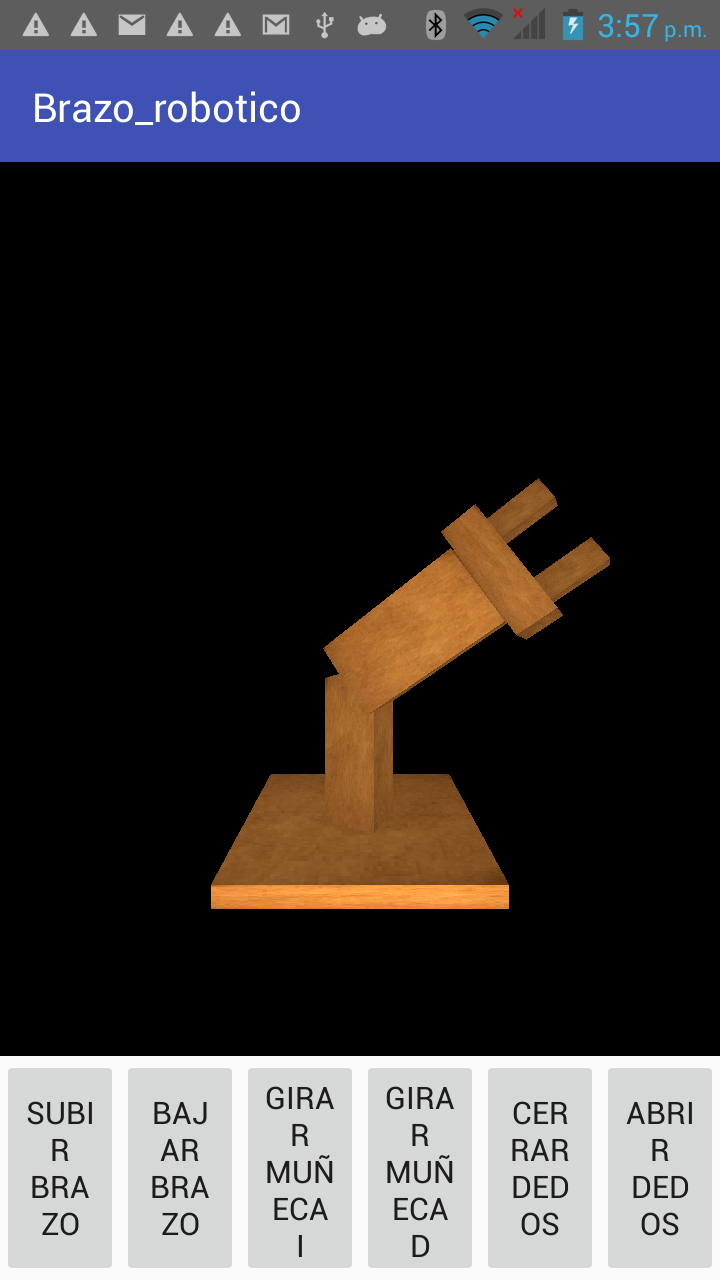
\includegraphics[width=0.98\textwidth]{Figs/brazoRobotico1}
		 \end{center}
	\end{column}
	\begin{column}{0.22\textwidth}  
		\begin{center}
		 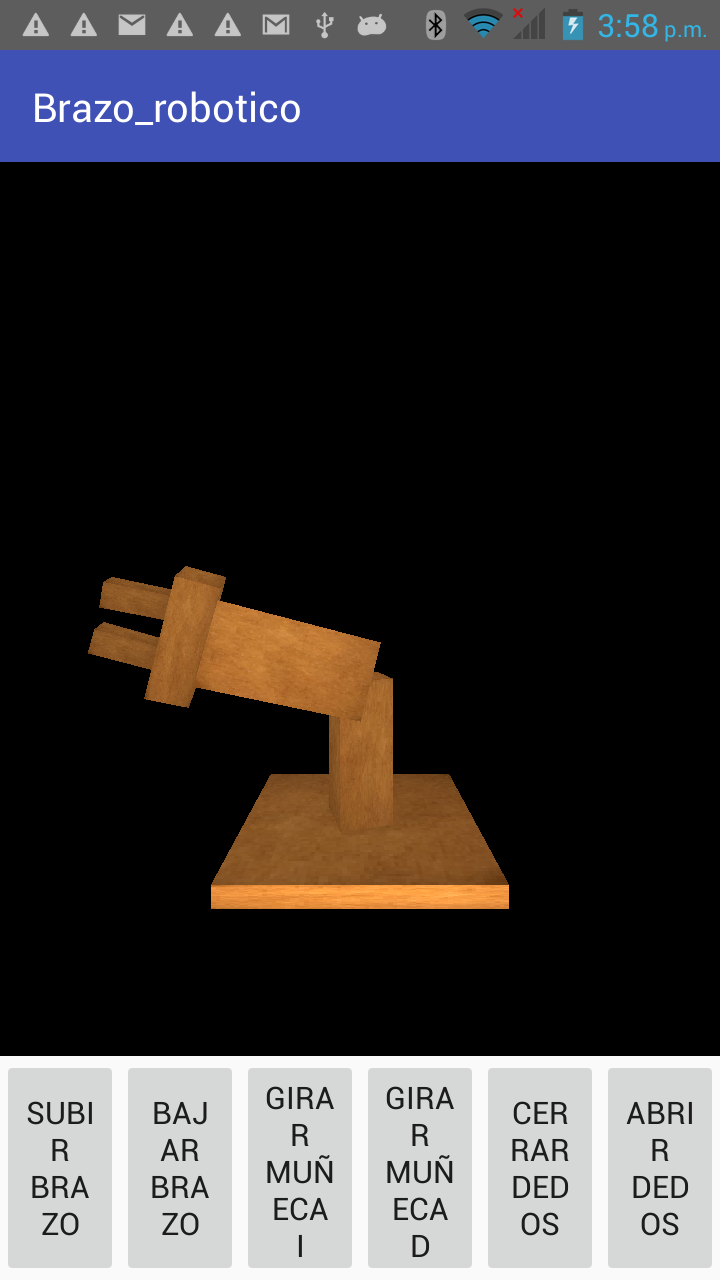
\includegraphics[width=0.98\textwidth]{Figs/brazoRobotico2}
		 \end{center}
	\end{column}
\end{columns}
%\end{block} 
\footnotetext[1]{\fullcite{\EntradaBibtex}}
\end{frame}

\renewcommand{\EntradaBibtex}{BrazoRobot_Uriegas2022}

\begin{frame}{\citetitle{\EntradaBibtex} \footnotemark[1] (1)}
\begin{columns}
\begin{column}{0.25\textwidth}  
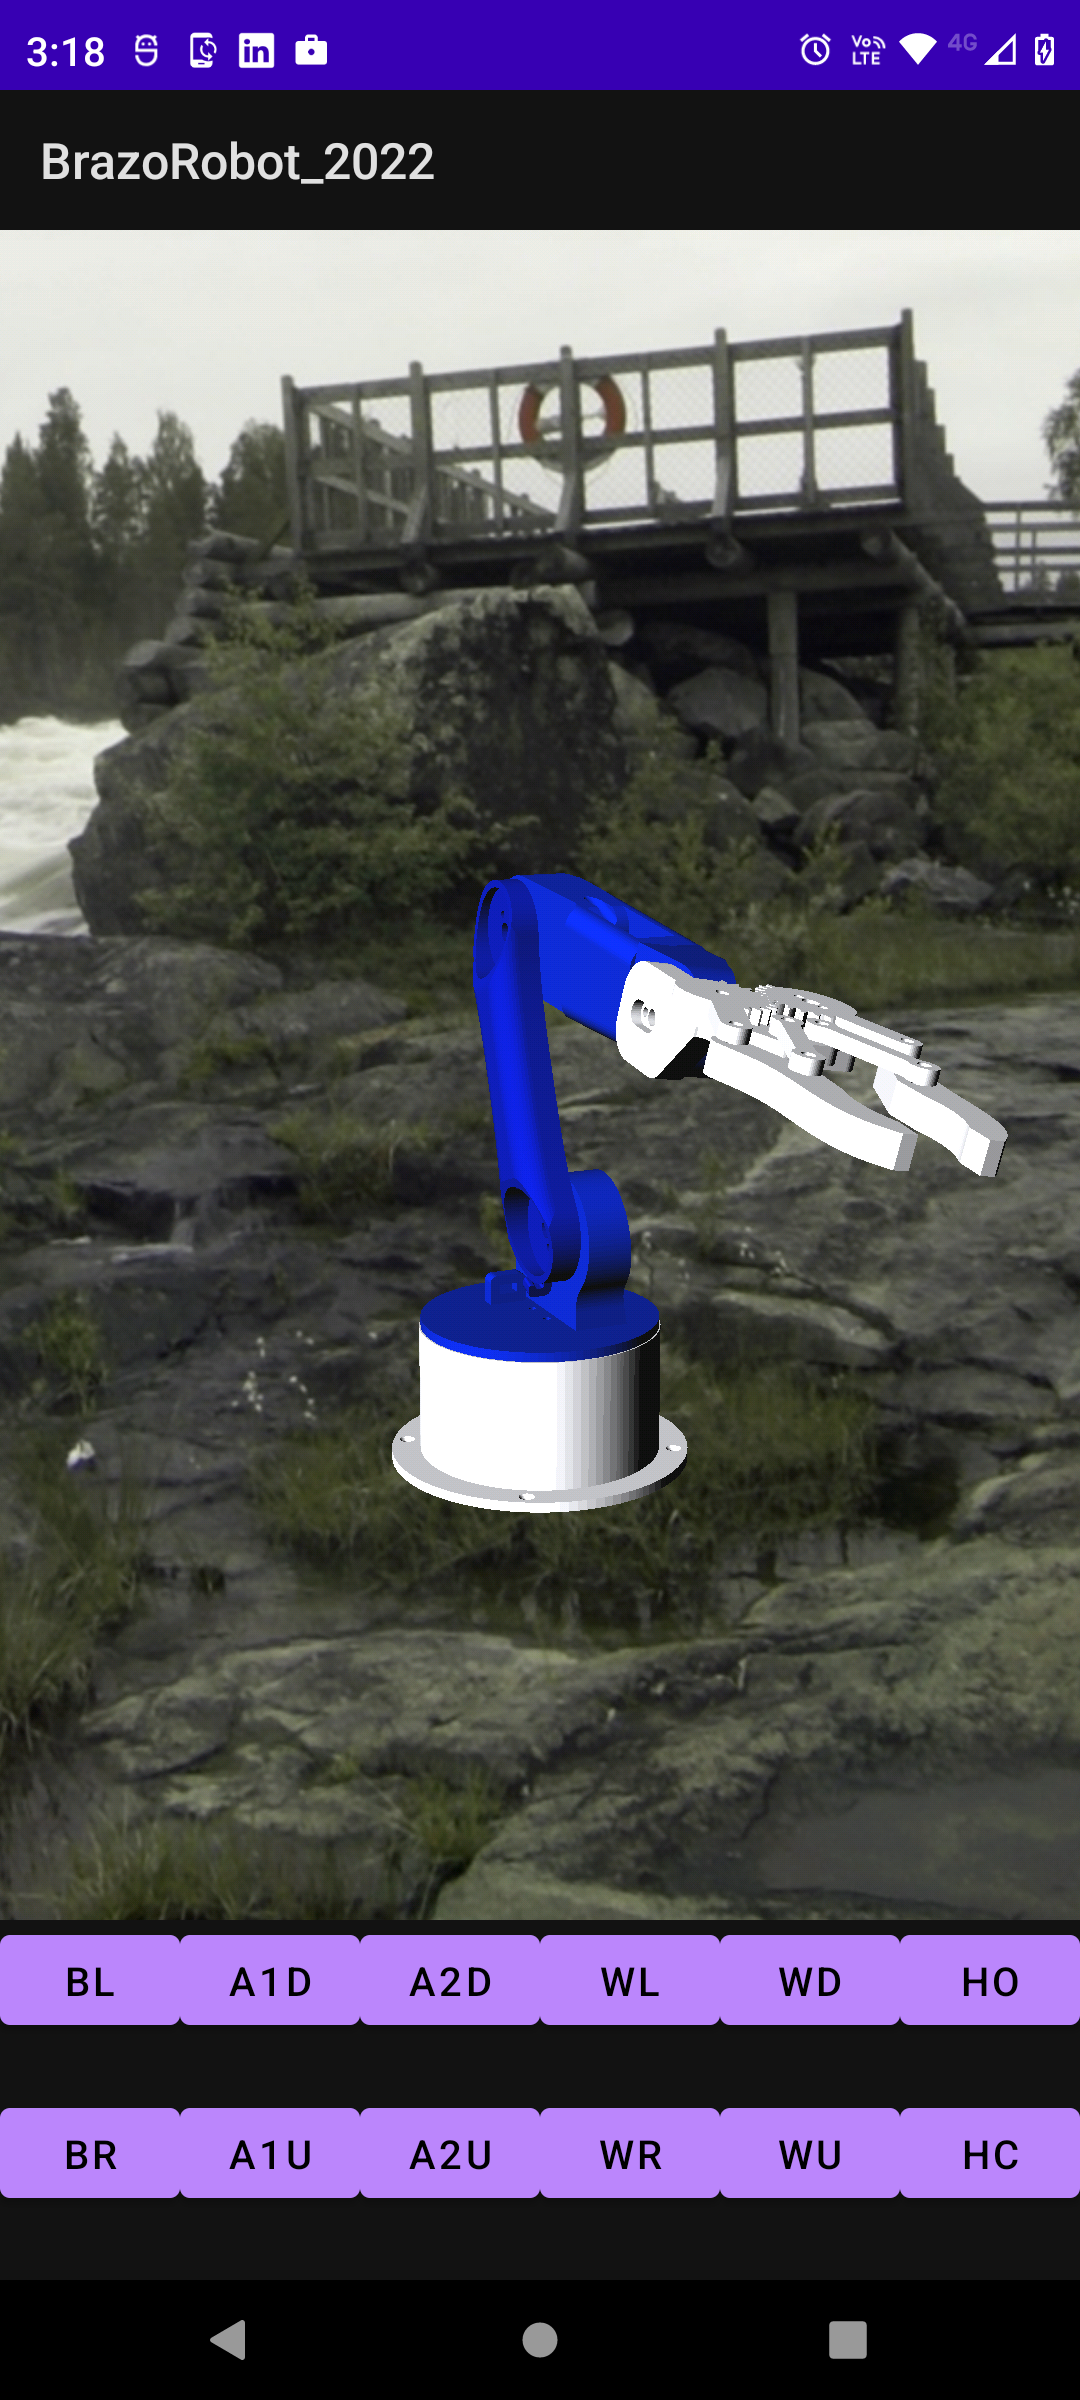
\includegraphics[width=0.82\textwidth]{2019_BrazoRobot3D/figs/BrazoRobot1}
\end{column}
\begin{column}{0.25\textwidth}  
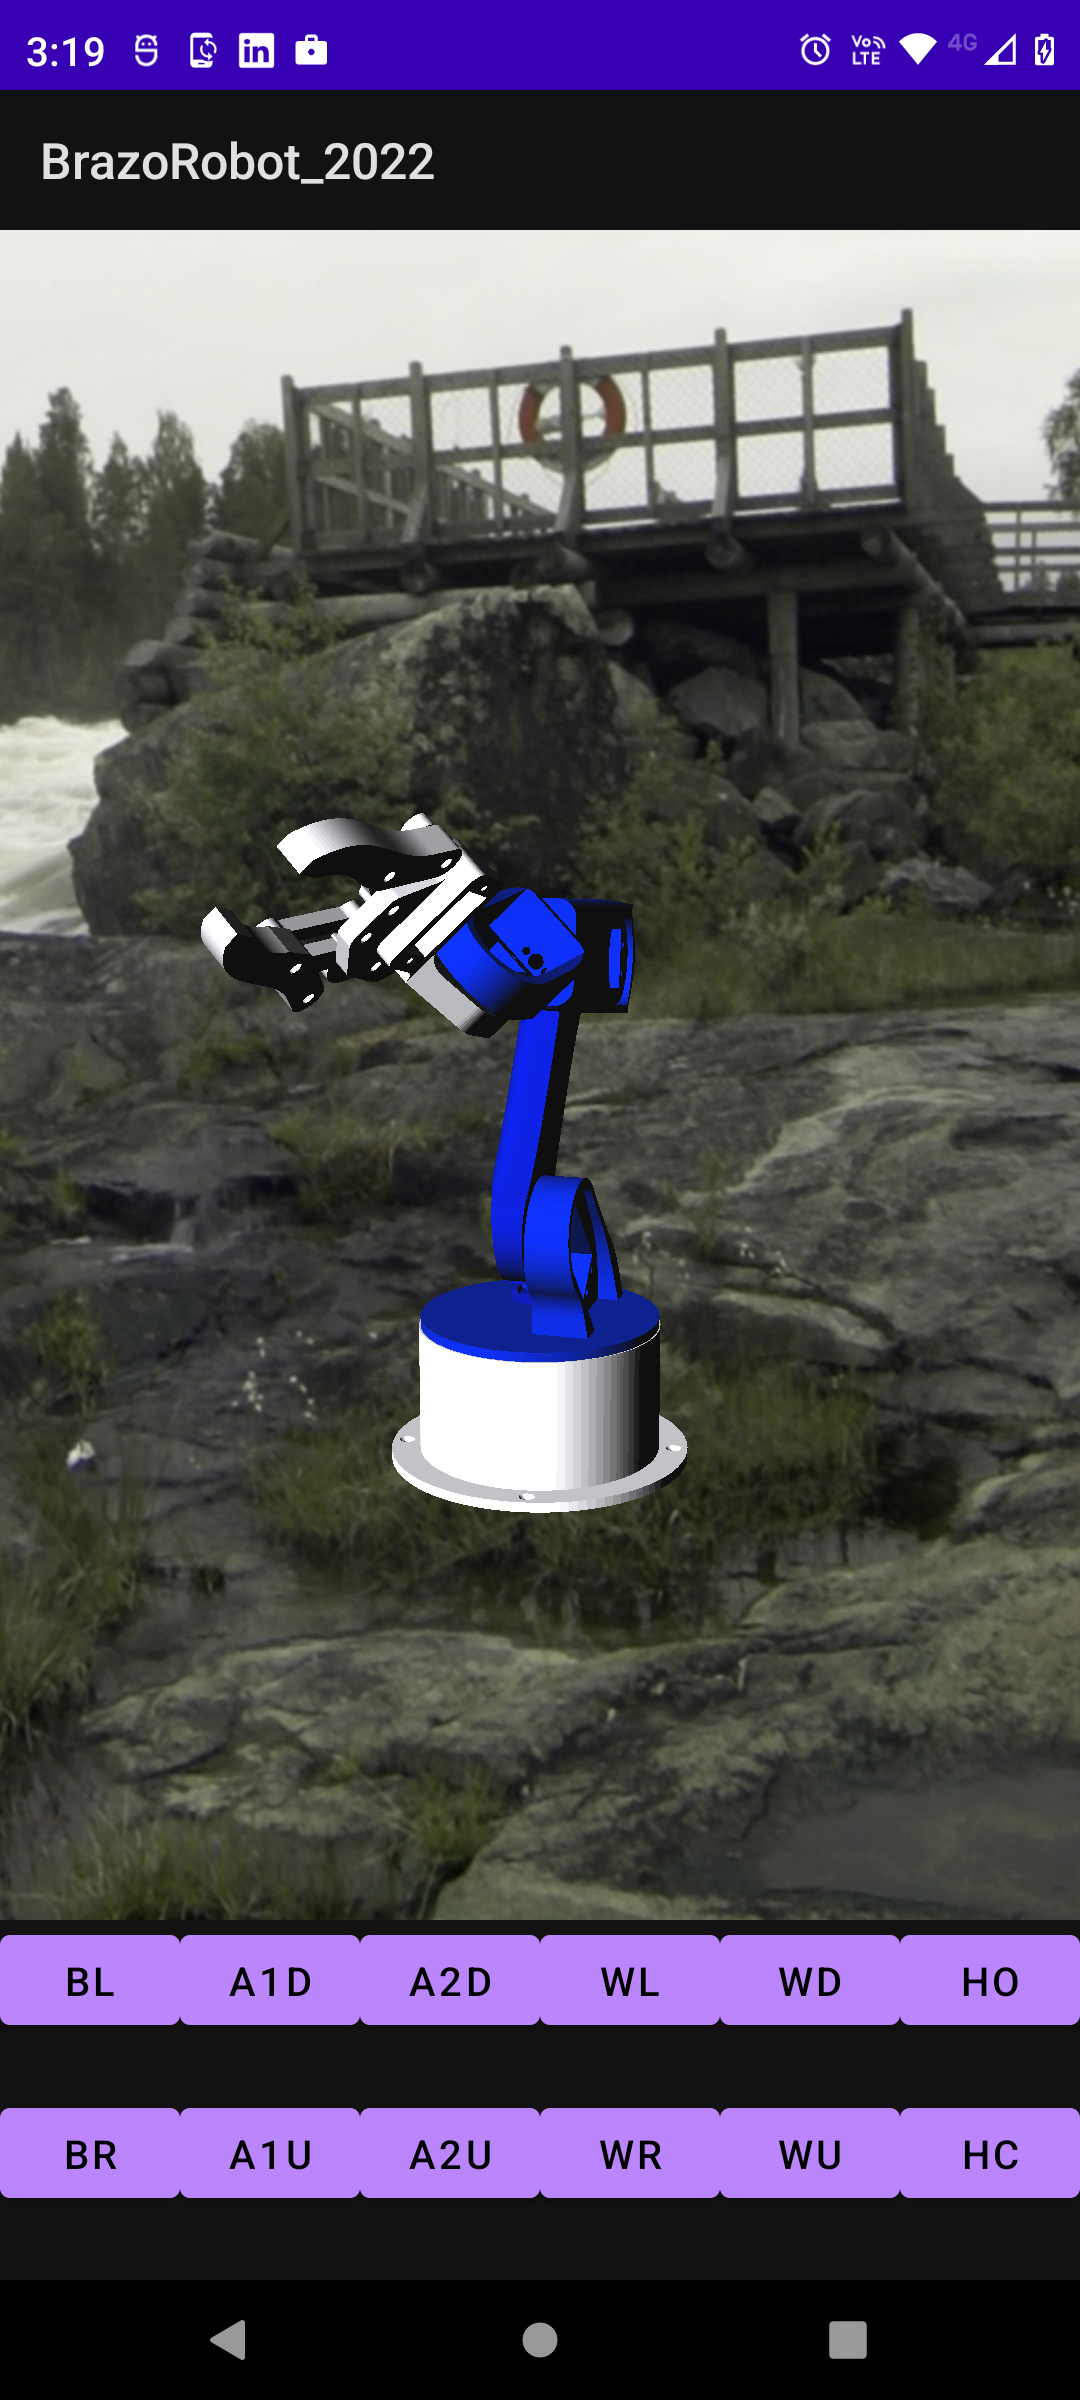
\includegraphics[width=0.82\textwidth]{2019_BrazoRobot3D/figs/BrazoRobot2}
\end{column}
\begin{column}{0.25\textwidth}  
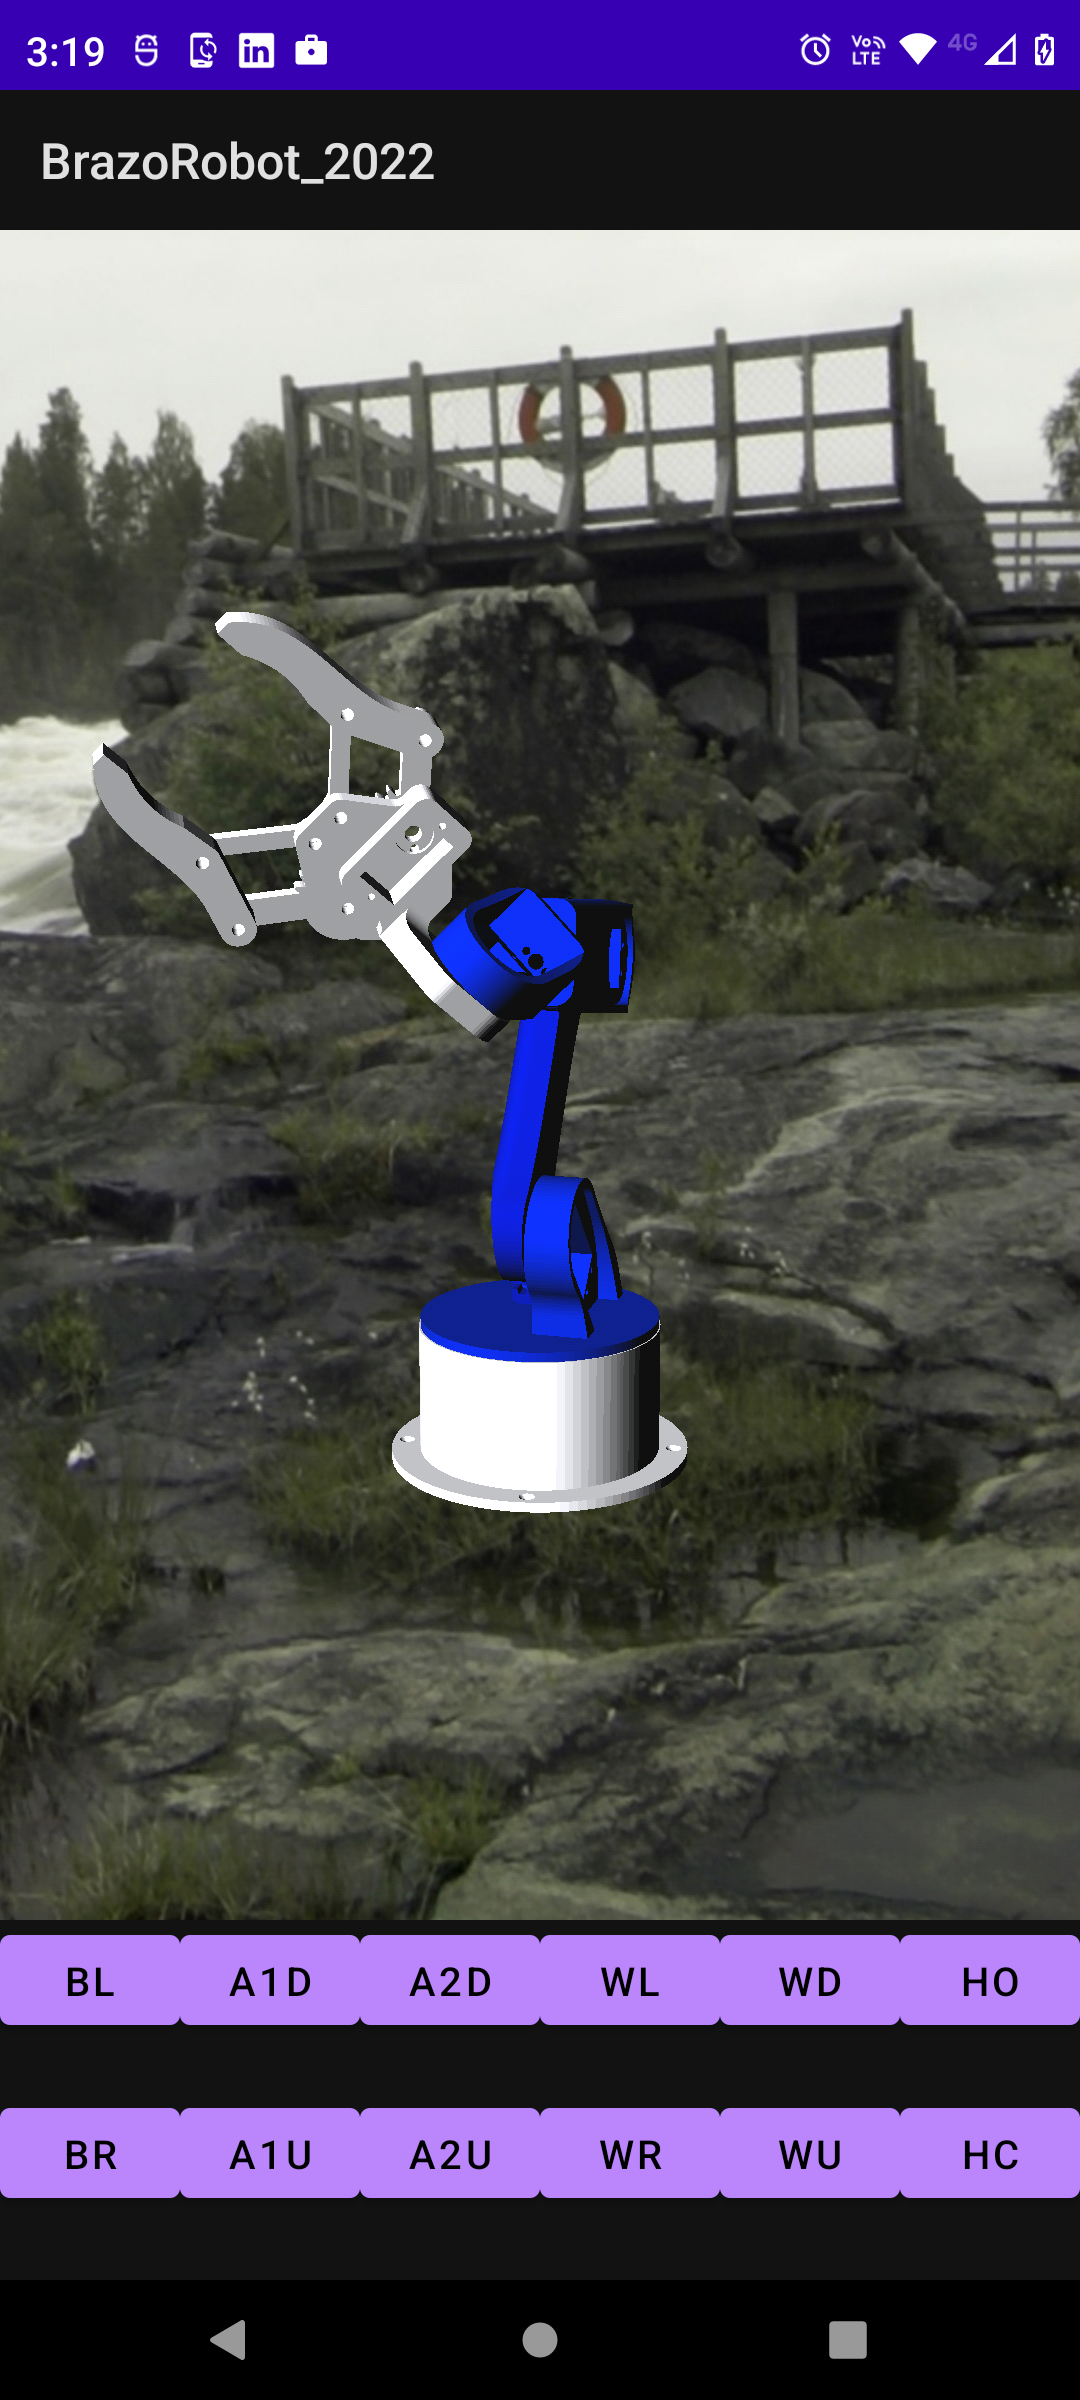
\includegraphics[width=0.82\textwidth]{2019_BrazoRobot3D/figs/BrazoRobot3}
\end{column}
\begin{column}{0.25\textwidth}  
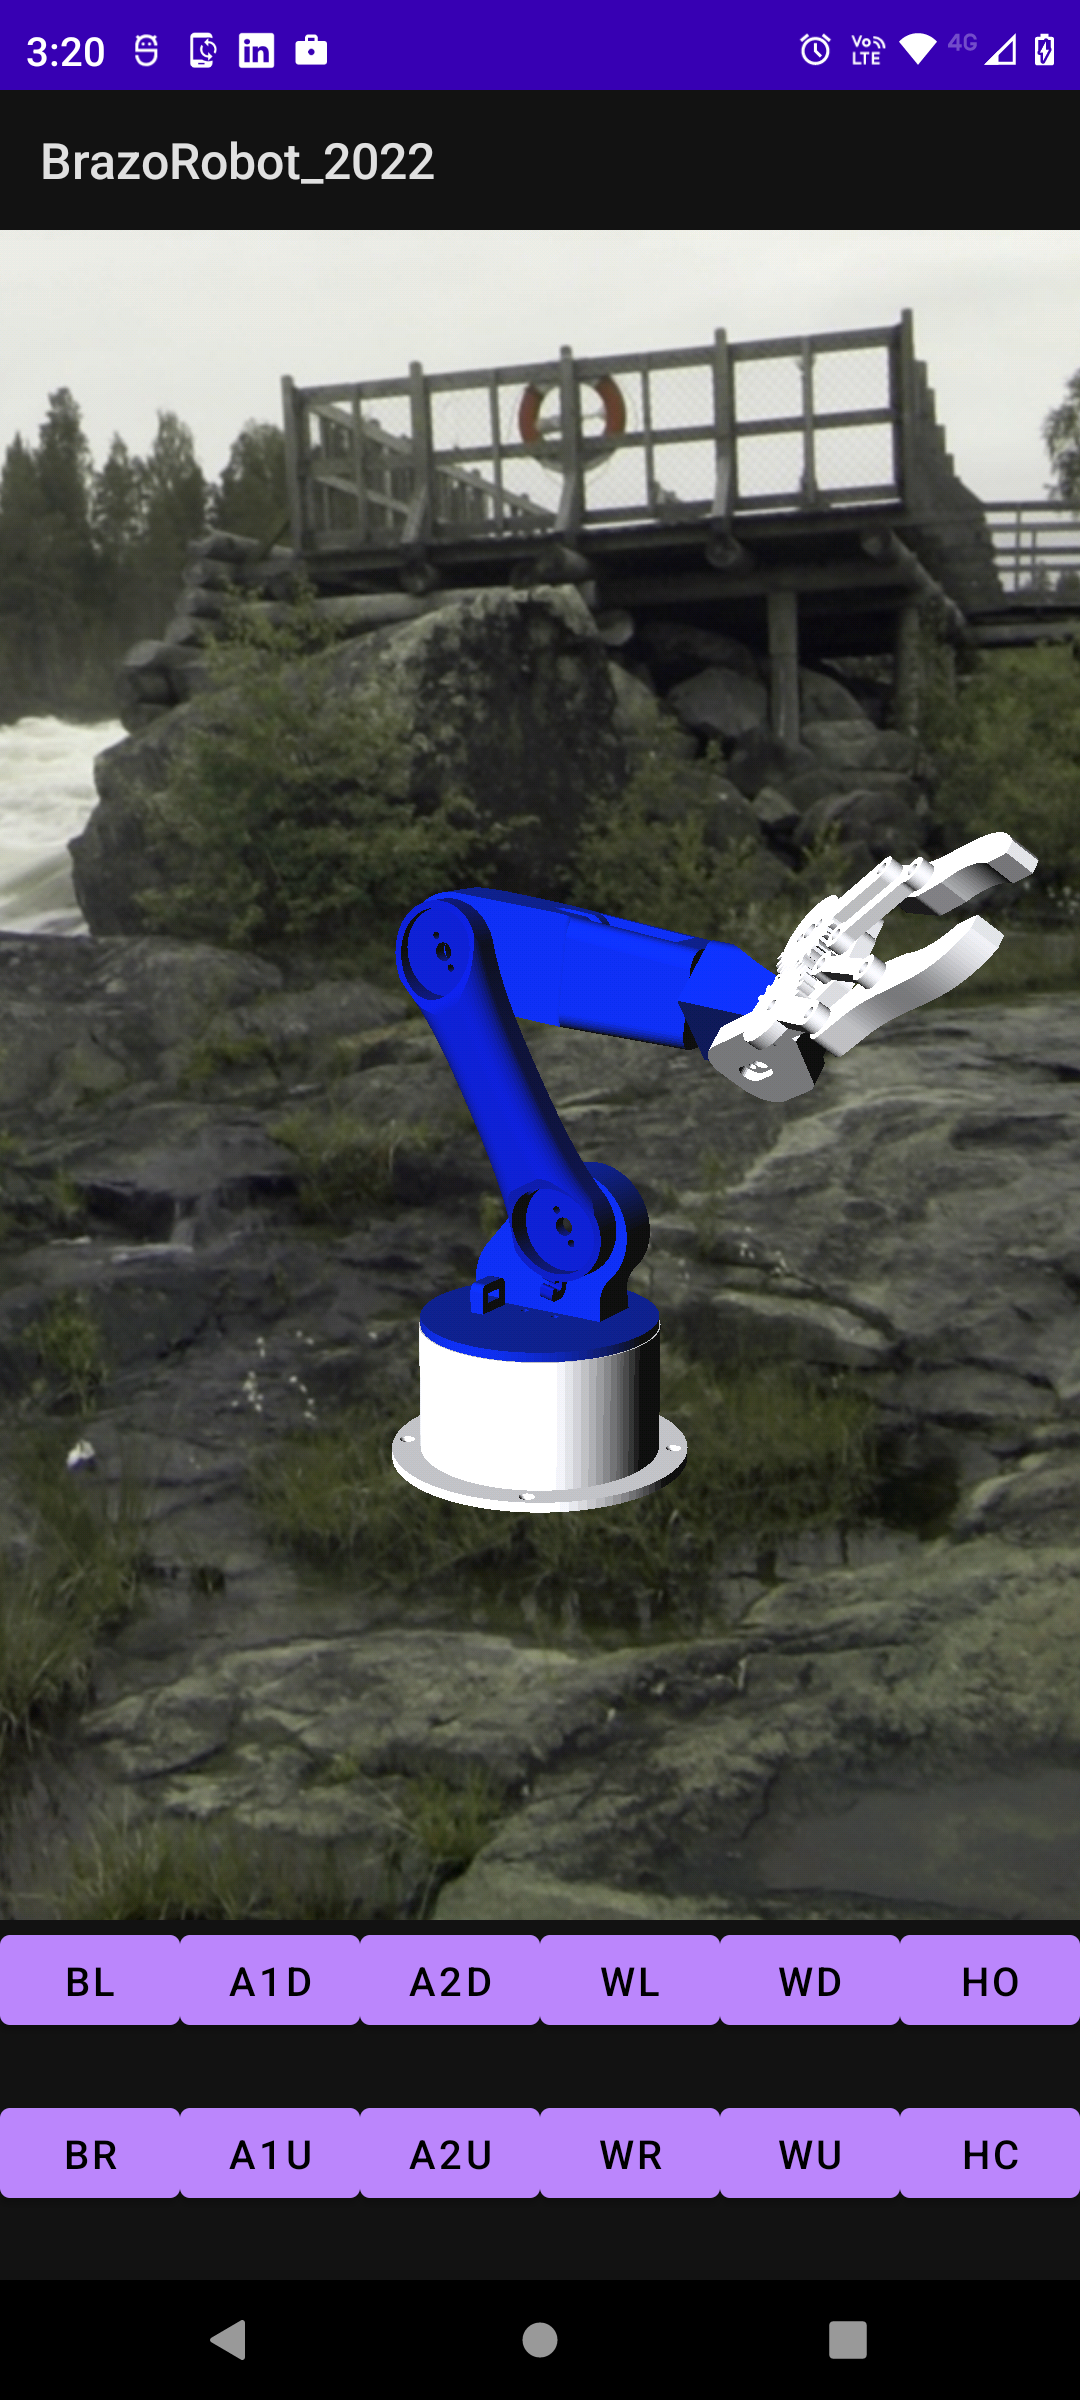
\includegraphics[width=0.82\textwidth]{2019_BrazoRobot3D/figs/BrazoRobot4}
\end{column}

\end{columns}
\footnotetext[1]{\fullcite{\EntradaBibtex}}
\end{frame}



\renewcommand{\EntradaBibtex}{Ajedrez3D_2017}
%\setcounter{footnote}{0}


\begin{frame}{\citetitle{\EntradaBibtex} \footnotemark[1] (1)}
%\begin{block}{Multiplayer Chess \footnotemark} 
\begin{columns}
\begin{column}{0.4\textwidth}
		\begin{itemize}
		\item Cada pieza fue modelada en Blender y exportada a la aplicación de Android
		\item Aplicación multidispositivo, que permite llevar una partida de ajedrez.
		\item El control del juego queda del lado del servidor. 
		\end{itemize}

\end{column}
\begin{column}{0.3\textwidth}
%   some text here some text here some text here some text here some text here
     \begin{center}
     %%%%% this is a minipage, so \textwidth is already adjusted to the size of the column
     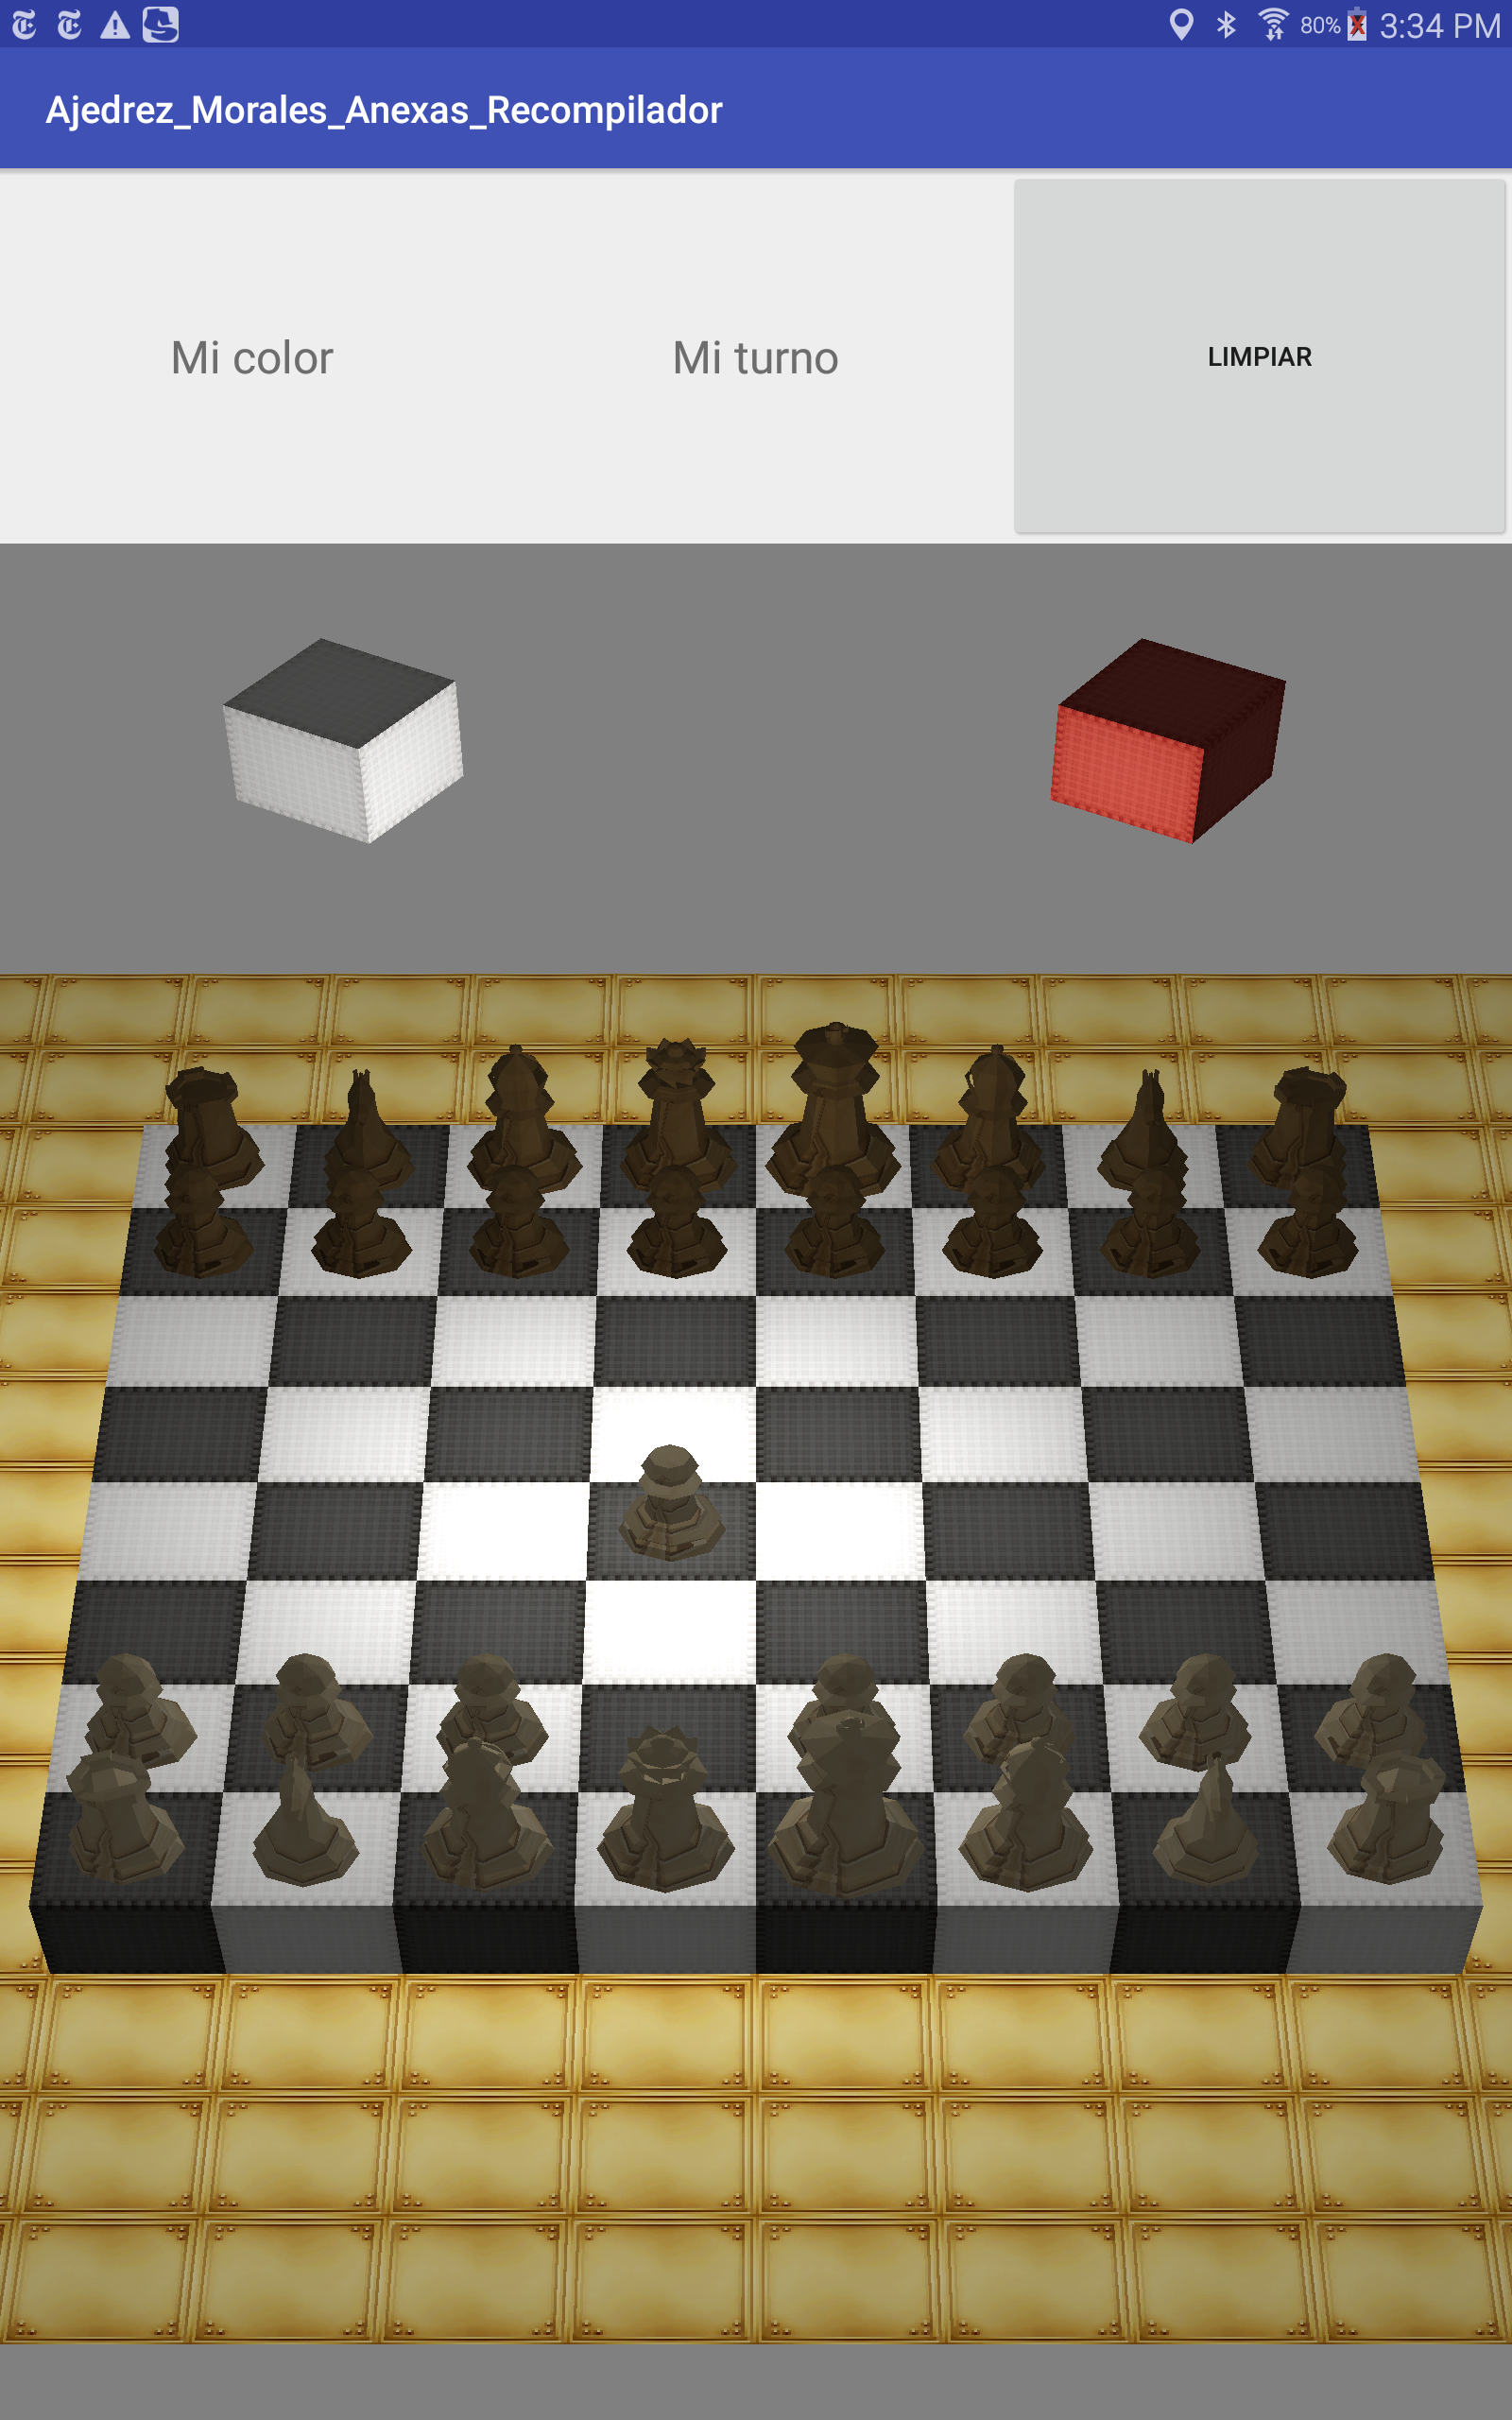
\includegraphics[width=0.7\textwidth]{Figs/Ajedrez_01}
     \end{center}

\end{column}
\begin{column}{0.3\textwidth}  
    \begin{center}
     %%%%% this is a minipage, so \textwidth is already adjusted to the size of the column
     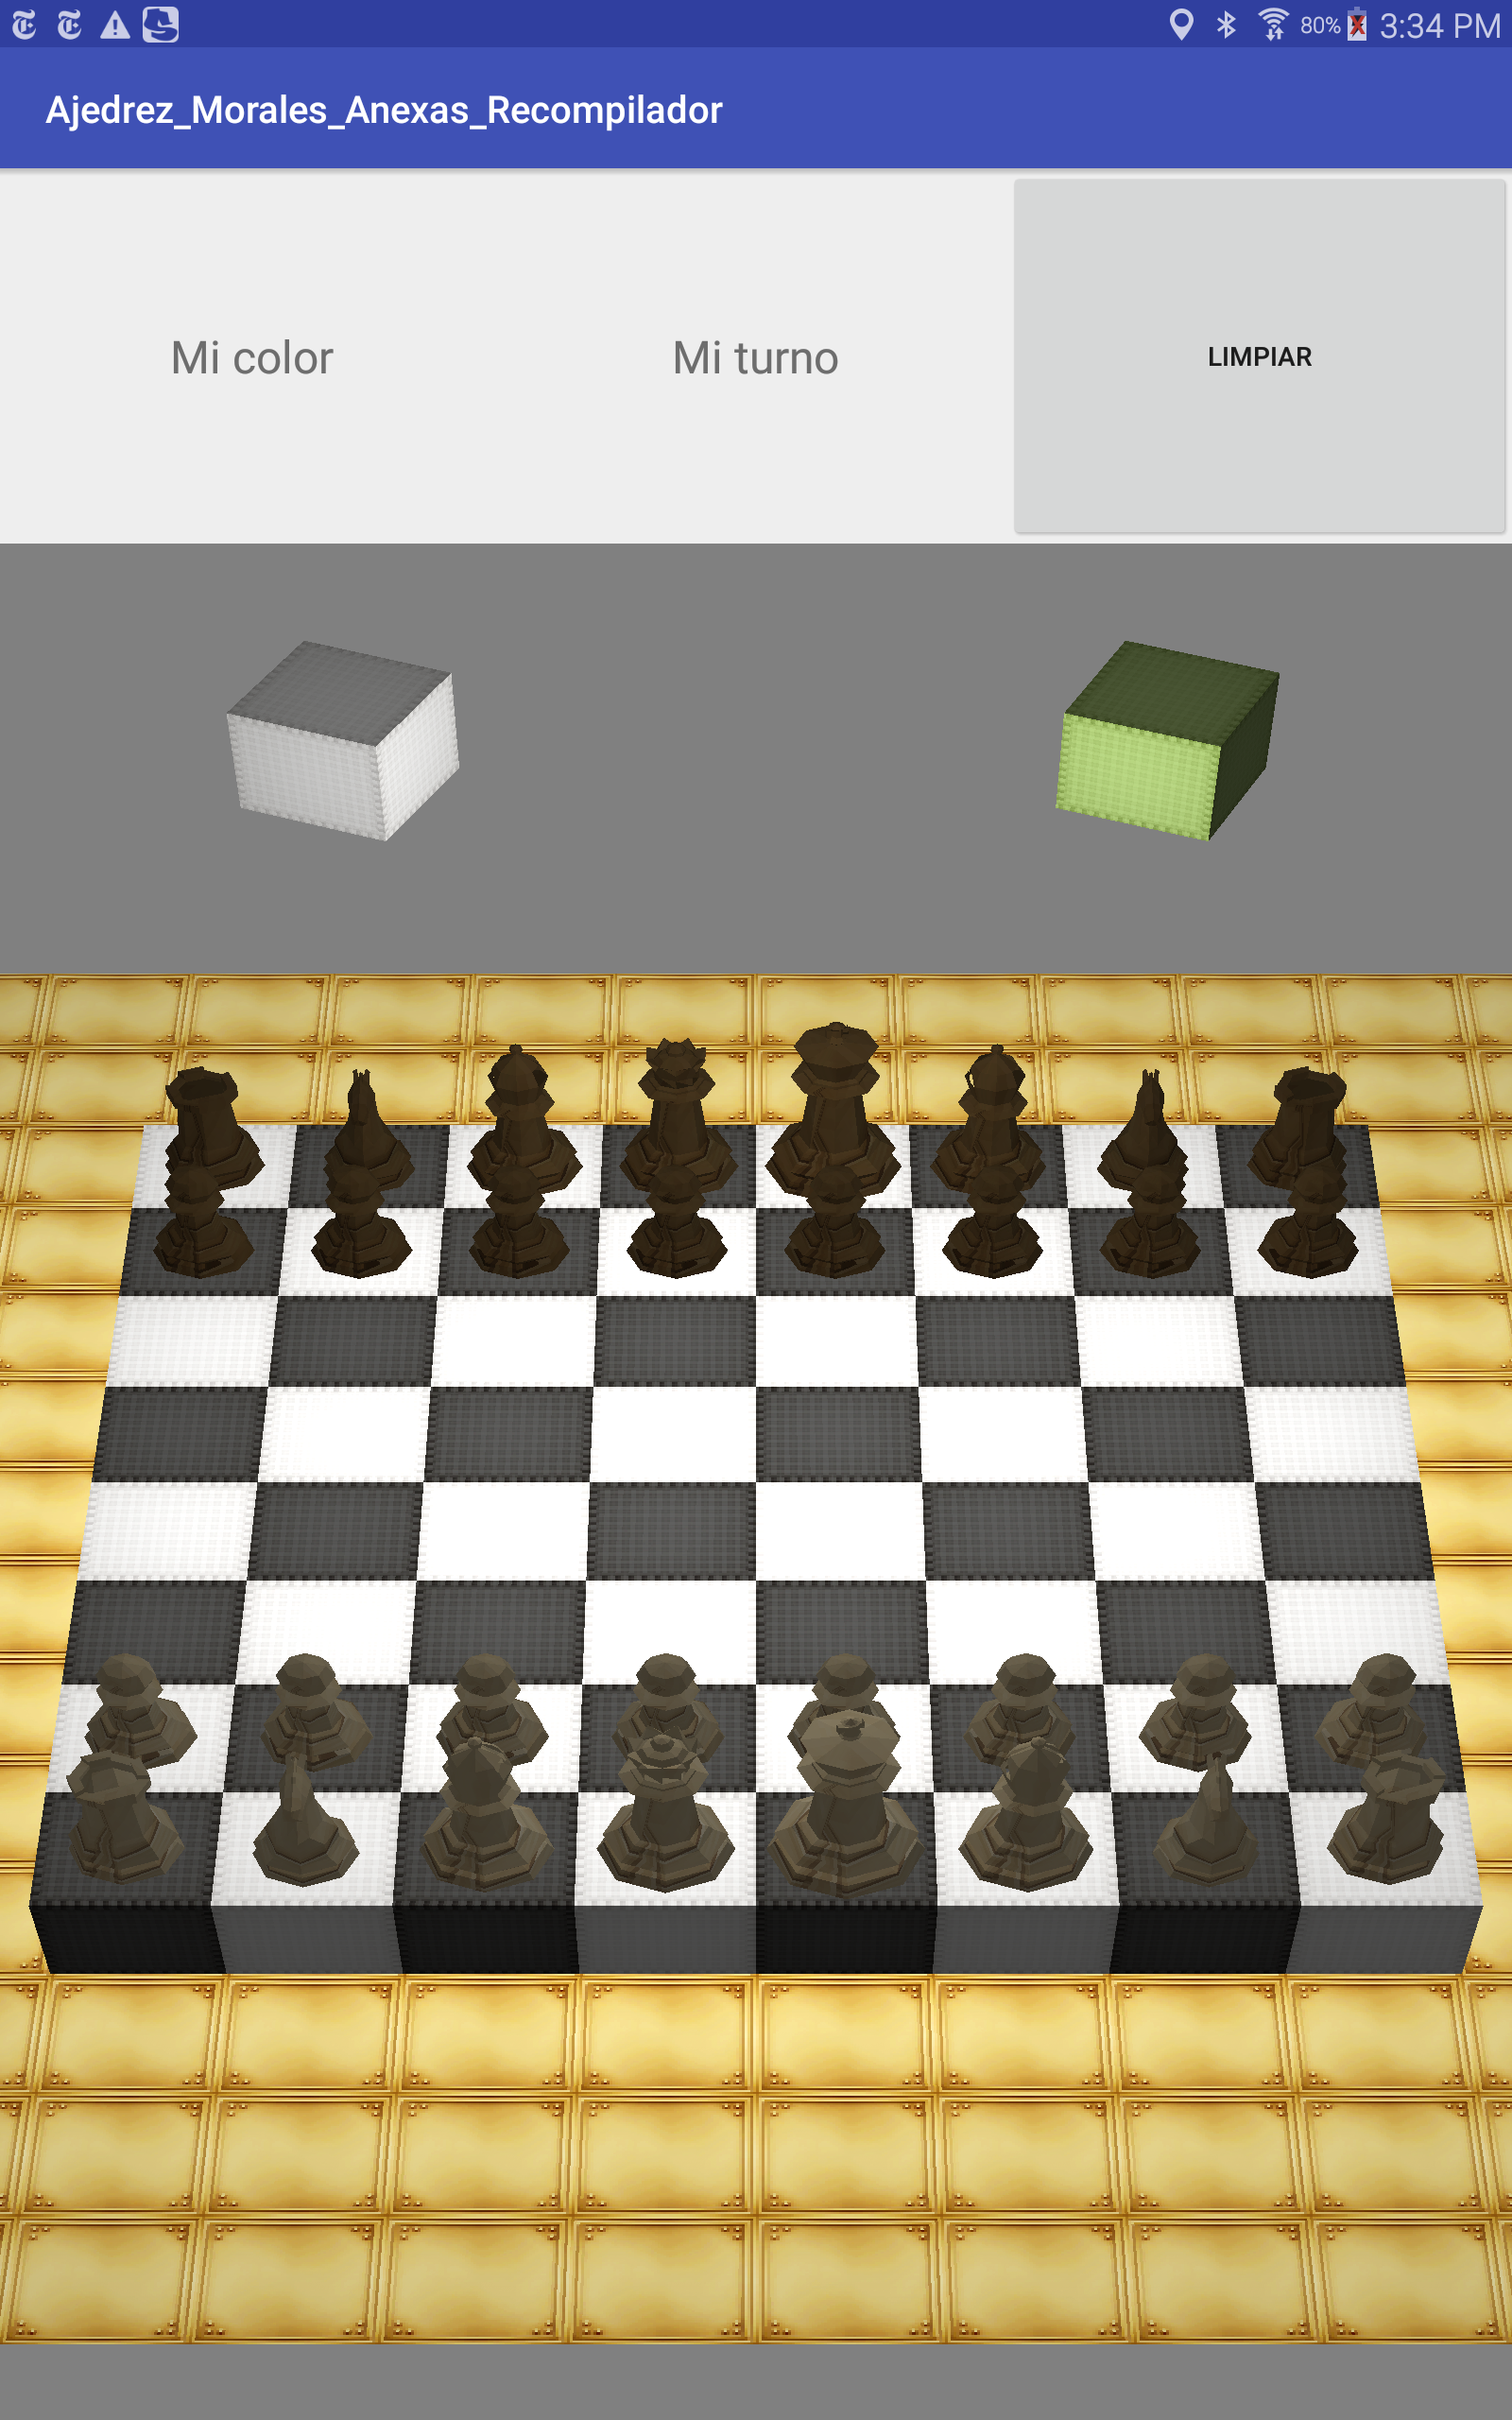
\includegraphics[width=0.7\textwidth]{Figs/Ajedrez_02}
     \end{center}
\end{column}
\end{columns}
%\footfullcite*{\EntradaBibtex}
\footnotetext[1]{\fullcite{\EntradaBibtex}}
\end{frame}



\renewcommand{\EntradaBibtex}{CruzdeMalta_2017}

\begin{frame}{\citetitle{\EntradaBibtex} \footnotemark[1] (1)}
%\begin{block}{Simulación del Mecanismo de la Cruz de Malta\footnotemark} 
	\begin{itemize}
	\item Se modelaron los componentes individuales 3D (cilindros, tetaedros, etc)
	\item Se incorporó texturas, iluminación y sombras
	\item Es posible ver el modelo desde múltiples perspectivas
	\end{itemize}
\begin{columns}
	\begin{column}{0.48\textwidth}
    \begin{center}
     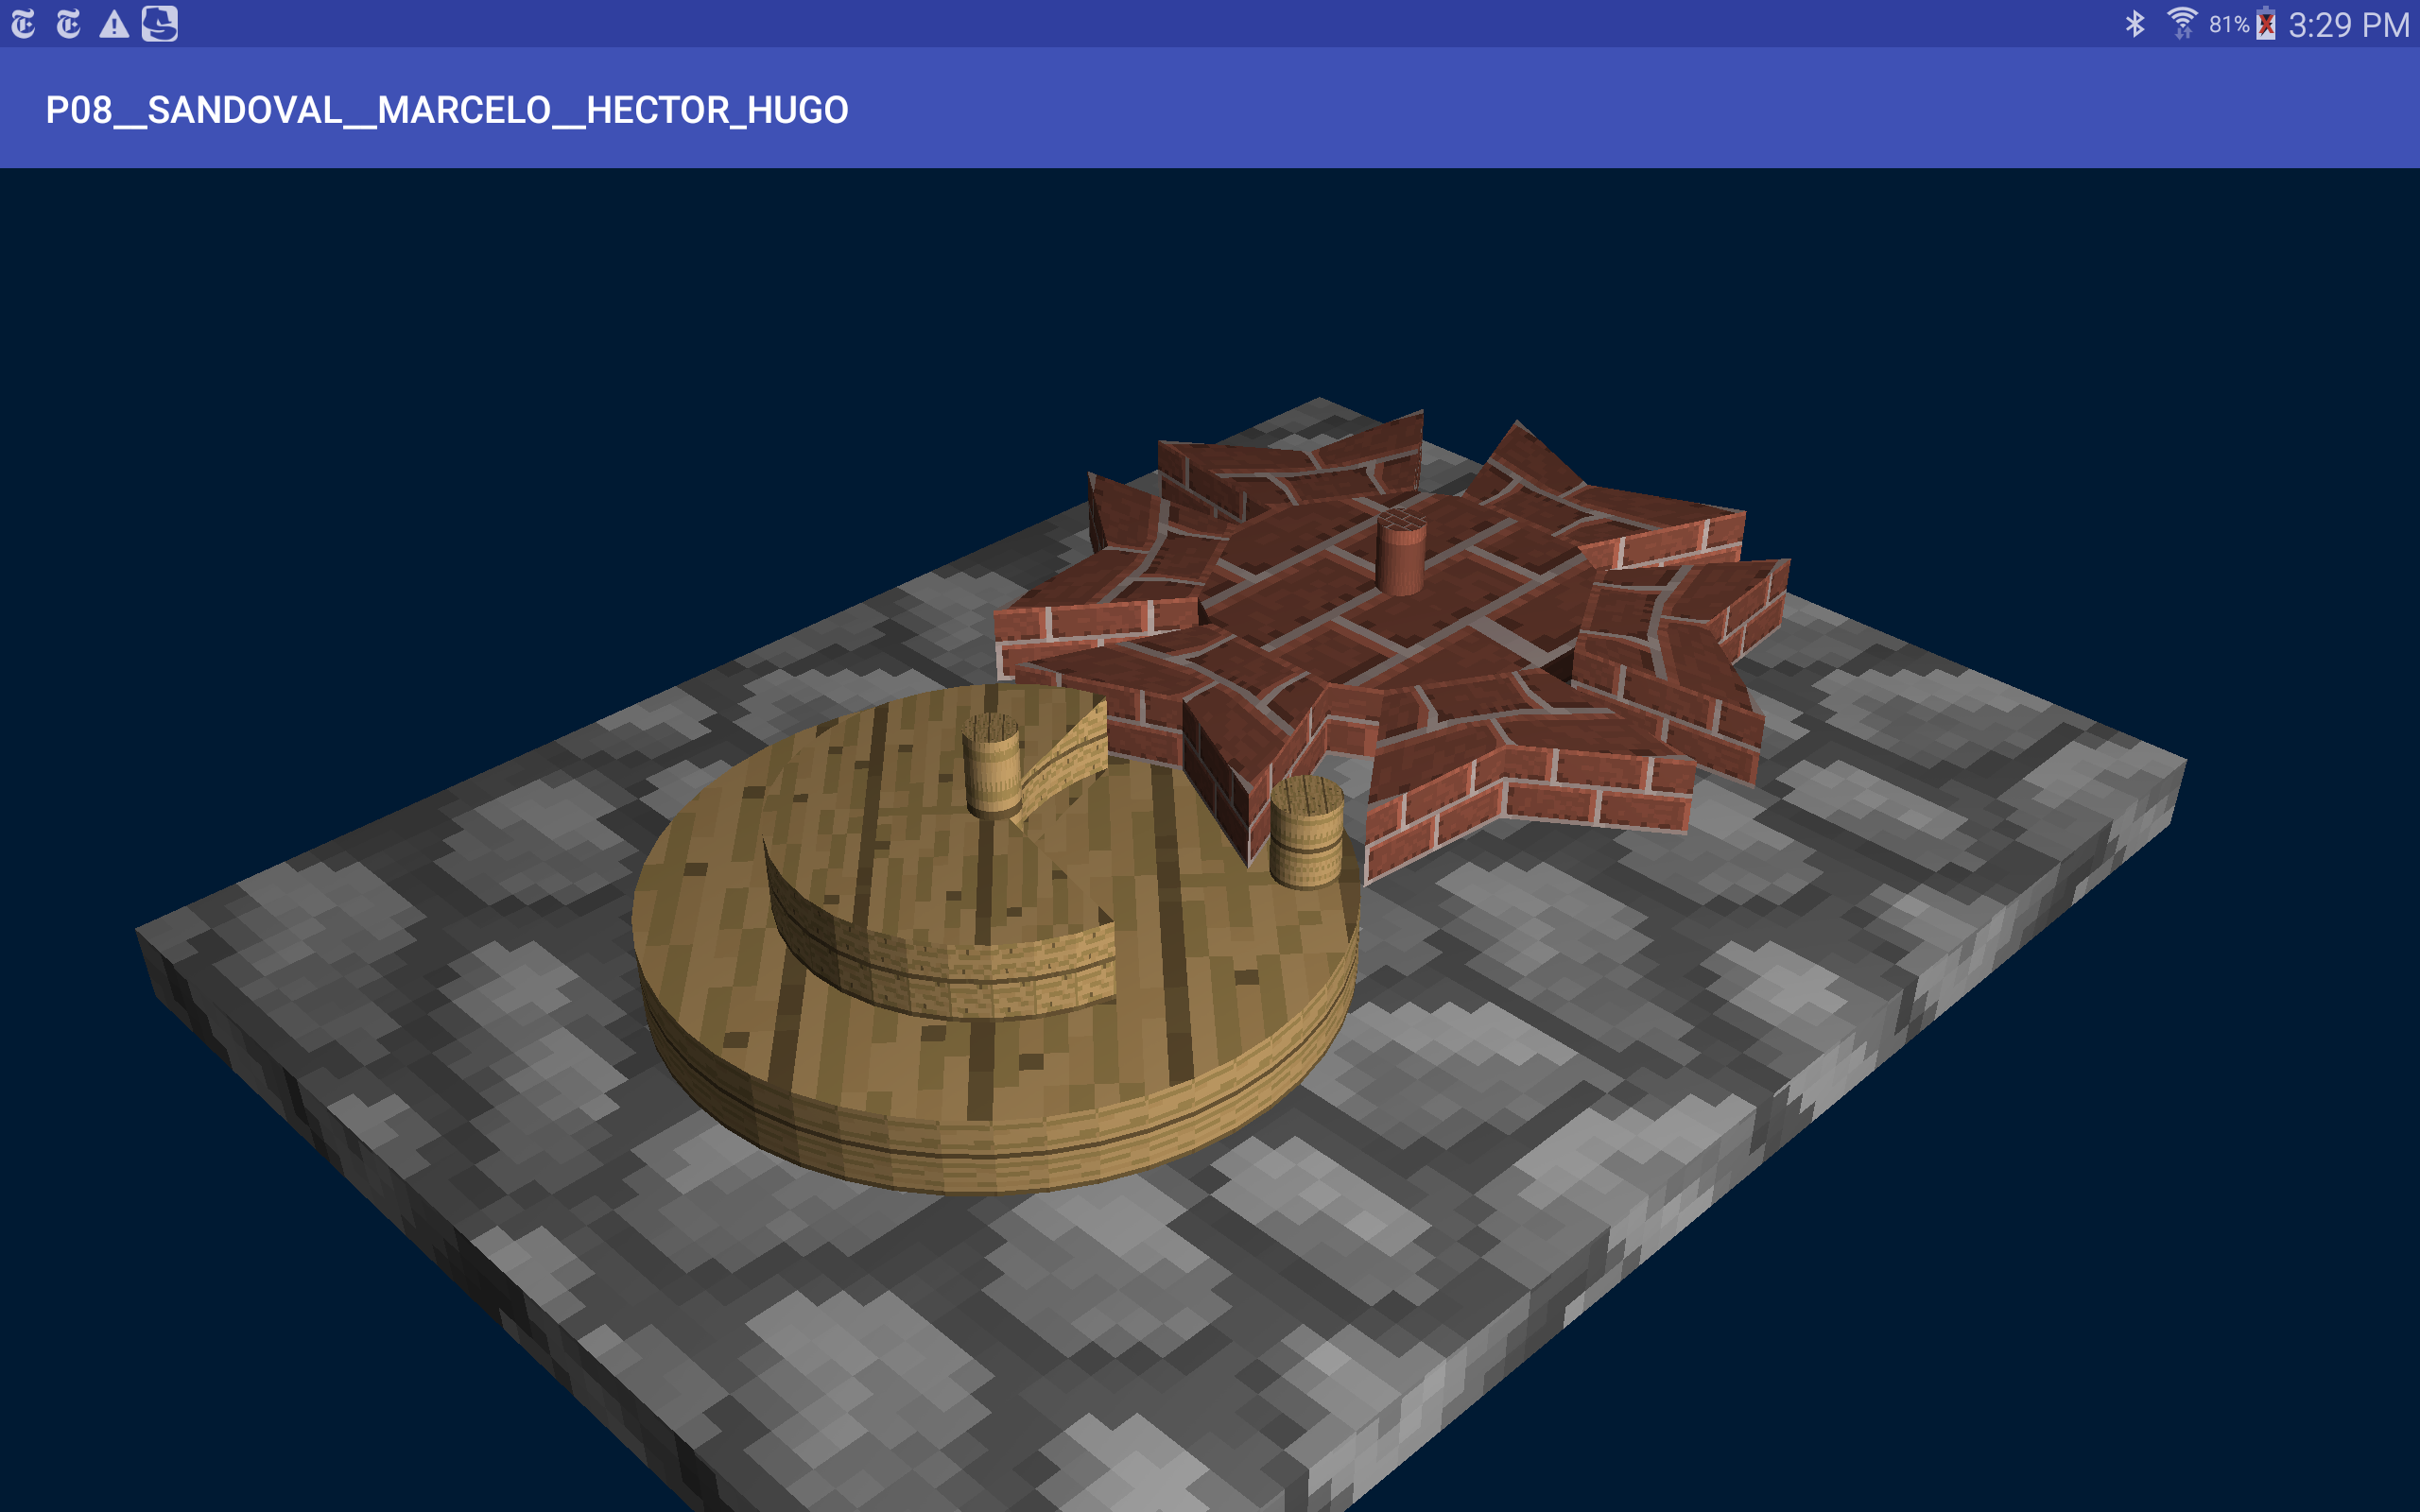
\includegraphics[width=0.7\textwidth]{Figs/CruzMalta_01}
     \end{center}
\end{column}
\begin{column}{0.48\textwidth}  
    \begin{center}
     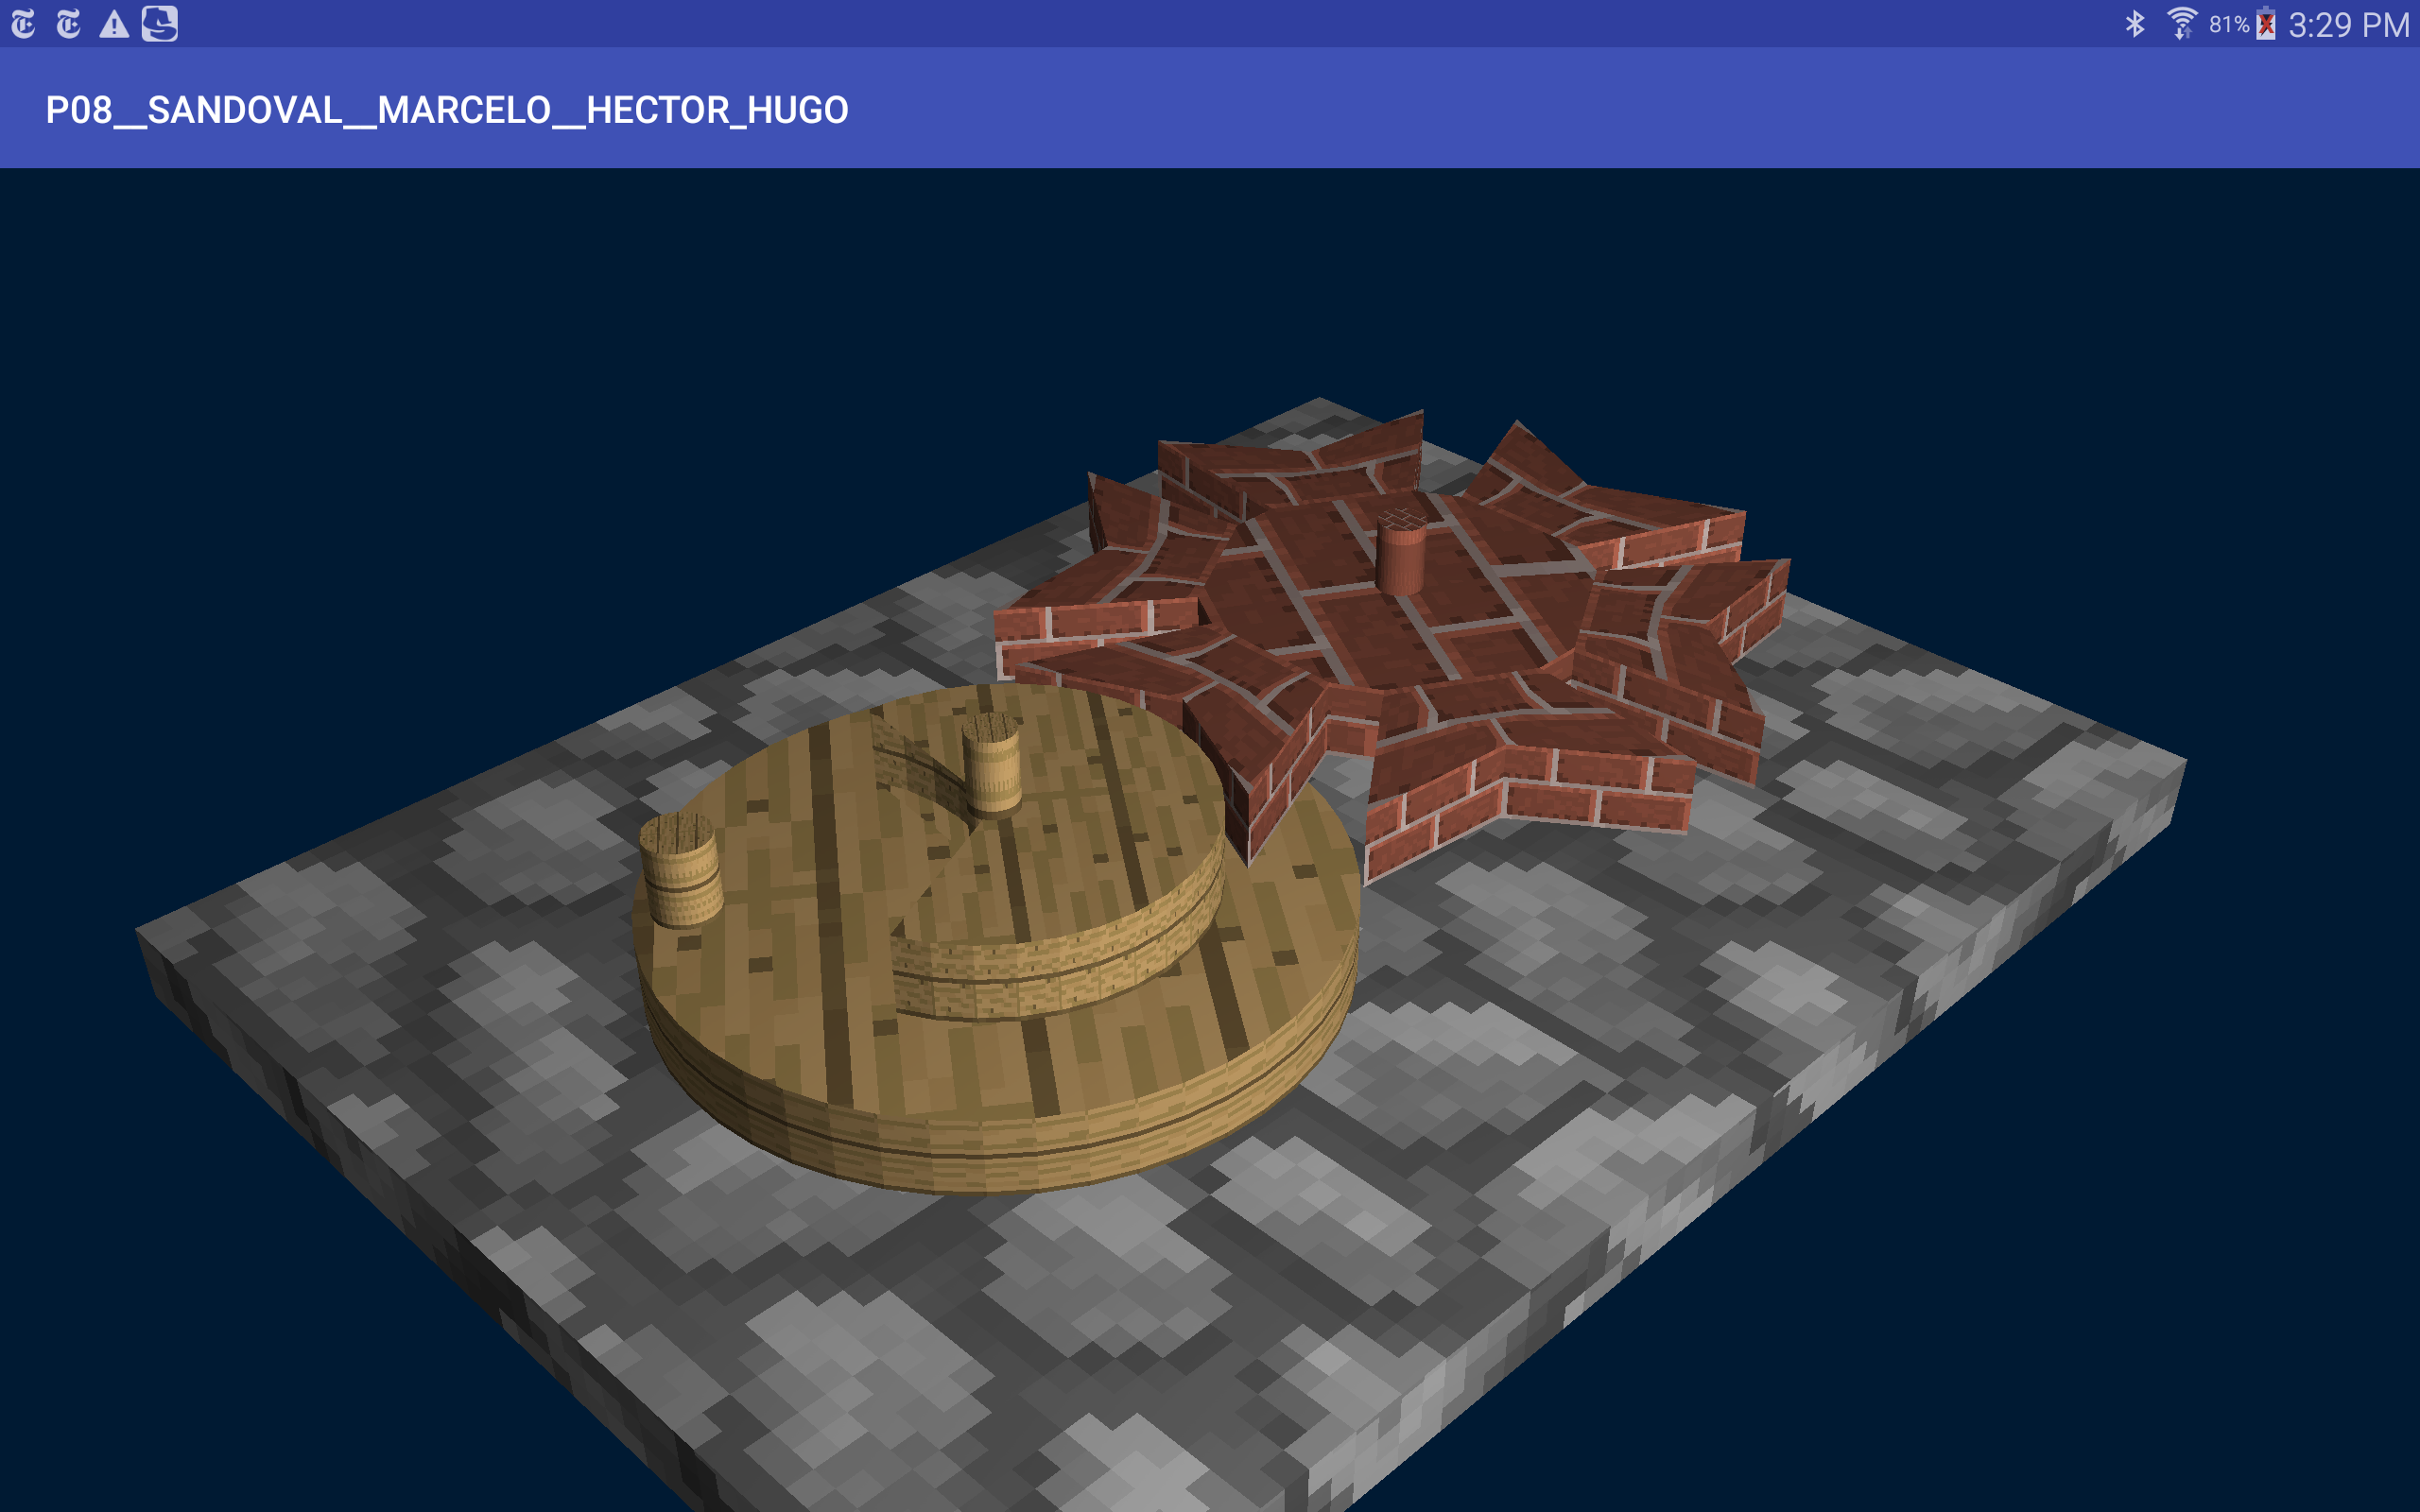
\includegraphics[width=0.7\textwidth]{Figs/CruzMalta_02}
     \end{center}
\end{column}
\end{columns}
%\end{block} 
\footnotetext[1]{\fullcite{\EntradaBibtex}}
%\footnotetext{Héctor Hugo Sandoval Marcelo. \textbf{Movimiento de la Cruz de Malta con Iluminación y Texturas con Java y OpenGL ES 2.0 en Android.}. Universidad Politécnica de Victoria,  Informe técnico proyecto de asignatura ``Graficación por Computadora Avanzada'', 2017. Sin Publicar.}
%\\setcounter{footnote}{0}
\end{frame}



\renewcommand{\EntradaBibtex}{JaguarAplicacionMovil_2020}
\begin{frame}{\citetitle{\EntradaBibtex} \footnotemark[1] (1)}


%\begin{frame}{Desarrollos Tecnológicos}
\begin{block}{-} 
\begin{columns}
\begin{column}{0.48\textwidth}
		\begin{itemize}
		\item Detección de Codigos QR
		\item Modelado de la mascota en 3D mediante el Software Blender
		\item Sobreposición del modelo 3D dependiendo de la posición del código QR
		\end{itemize}
	\end{column}
	\begin{column}{0.52\textwidth}  
	    \begin{center}
	    	 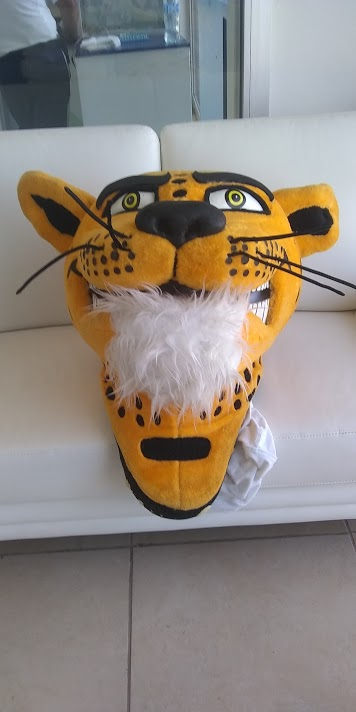
\includegraphics[width=0.25\textwidth]{Figs/JaguarFisico01}
	    	 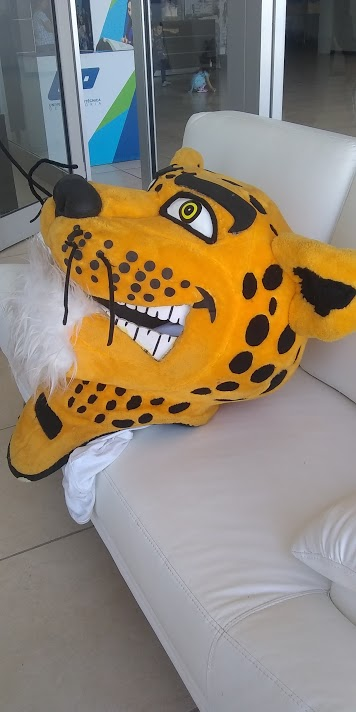
\includegraphics[width=0.25\textwidth]{Figs/JaguarFisico02}\\
    	 \end{center}
	\end{column}
	\end{columns}
	\end{block} 
	%\footnotetext{\fullcite{JaguarAplicacionMovil_2020}}
\footnotetext[1]{\fullcite{\EntradaBibtex}}
%\footnotetext{Andrés García González, Cristian Aléxis Lazo García, Damaris Mendoza Vázquez.  \textbf{Modelo 3D del Jaguar de la UPV sobre un código QR}. Universidad Politécnica de Victoria,  Informe técnico proyecto de asignatura ``Graficación por Computadora Aavanzada'', 2020. Sin Publicar.}
%\\setcounter{footnote}{0}
\end{frame}


\begin{frame}{\citetitle{\EntradaBibtex} (2)}
\begin{block}{-} 
\begin{columns}
	\begin{column}{0.98\textwidth}
	    \begin{center}
	    	 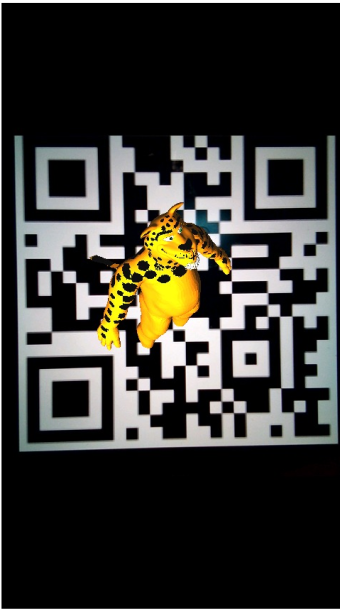
\includegraphics[width=0.24\textwidth]{Figs/JaguarVirtual01}
	    	 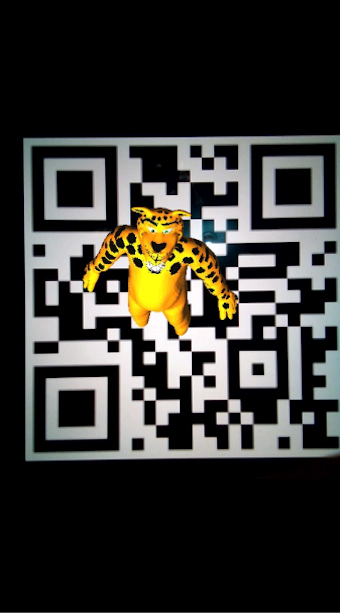
\includegraphics[width=0.24\textwidth]{Figs/JaguarVirtual02}
	    	 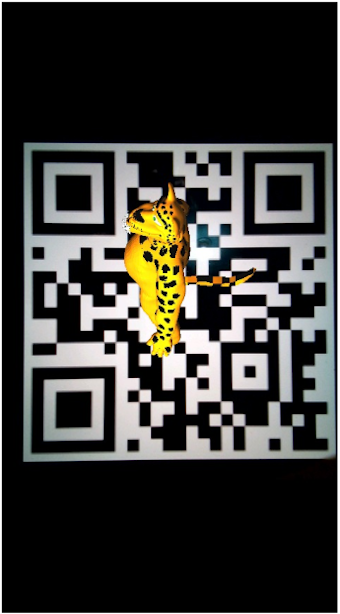
\includegraphics[width=0.24\textwidth]{Figs/JaguarVirtual03}
	    	 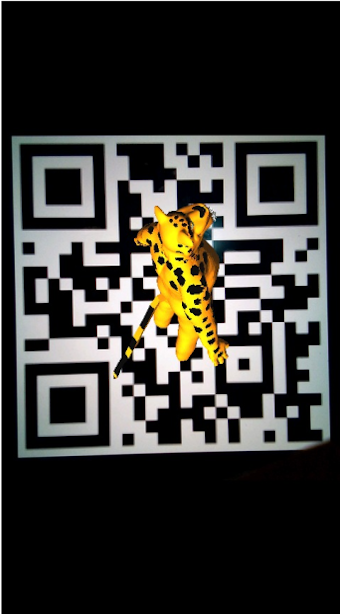
\includegraphics[width=0.24\textwidth]{Figs/JaguarVirtual04}
    	 \end{center}
	\end{column}
	\end{columns}
	\end{block} 
\end{frame}



\renewcommand{\EntradaBibtex}{RealidadAumentada_PrimerPrototipo_2019}
\begin{frame}{\citetitle{\EntradaBibtex} \footnotemark[1] (1)}

%\begin{frame}{Sistema de Realidad Aumentada \footnotemark}
%\begin{block}{Sistema de Realidad Aumentada \footnotemark} 
\begin{columns}
\begin{column}{0.48\textwidth}
		\begin{itemize}
		\item Detección de Codigos QR
		\item Decodificación del texto codificado en el codigo QR
		\item Sobreposición del modelo 3D dependiendo de la posición del código QR
		\end{itemize}
	\end{column}
	\begin{column}{0.52\textwidth}  
	    \begin{center}
	    	 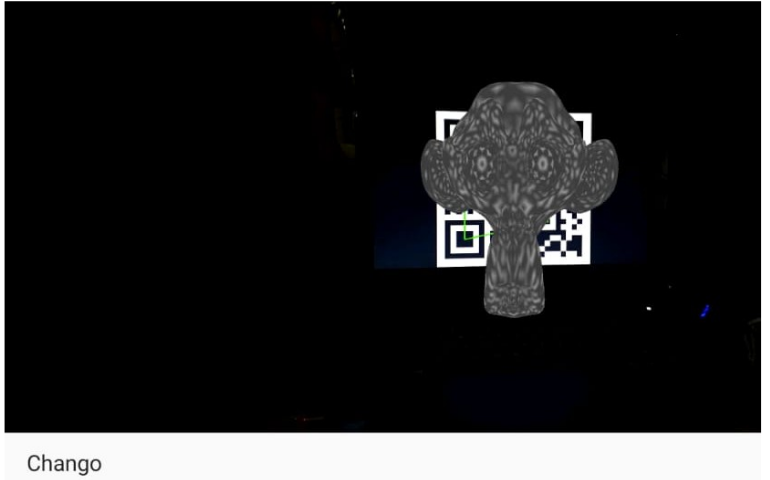
\includegraphics[width=0.95\textwidth]{Figs/SistemaAR1}
    	 \end{center}
	\end{column}
	\end{columns}
%	\end{block} 
\footnotetext[1]{\fullcite{\EntradaBibtex}}
%\footnotetext{Cárdenas Castillo Jesús Alfredo, Molina Pastrana Ana Karen, Ramos Lucio Eluis Carlo, Rodríguez Terán Linda Margarita y Vázquez Luna César Jovany.  \textbf{Visión por Computadora para Realidad Aumentada}. Universidad Politécnica de Victoria,  Informe técnico proyecto de asignatura ``Cómputo en Dispositivos Móviles'', 2019. Sin Publicar.}
%\\setcounter{footnote}{0}
\end{frame}

%Cárdenas Castillo Jesús Alfredo, Molina Pastrana Ana Karen, Ramos Lucio Eluis Carlo, Rodrı́guez Terán Linda Margarita, Vázquez Luna Cesar Jovany.
% \textbf{Visión por Computadora para Realidad Aumentada}. Universidad Politécnica de Victoria,  Informe técnico proyecto de asignatura ``Cómputo en Dispositivos Móviles'', 2019. Sin Publicar.

\begin{frame}{\citetitle{\EntradaBibtex} (2)}
%\begin{block}{Sistema de Realidad Aumentada (2)} 
\begin{columns}
\begin{column}{0.5\textwidth}
    \begin{center}
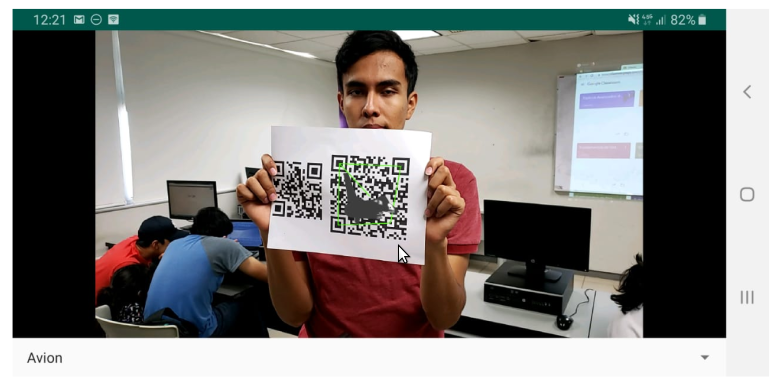
\includegraphics[width=0.98\textwidth]{Figs/SistemaAR2}\\
     \end{center}

\end{column}
\begin{column}{0.5\textwidth}  
    \begin{center}
\begin{itemize}
\end{itemize}

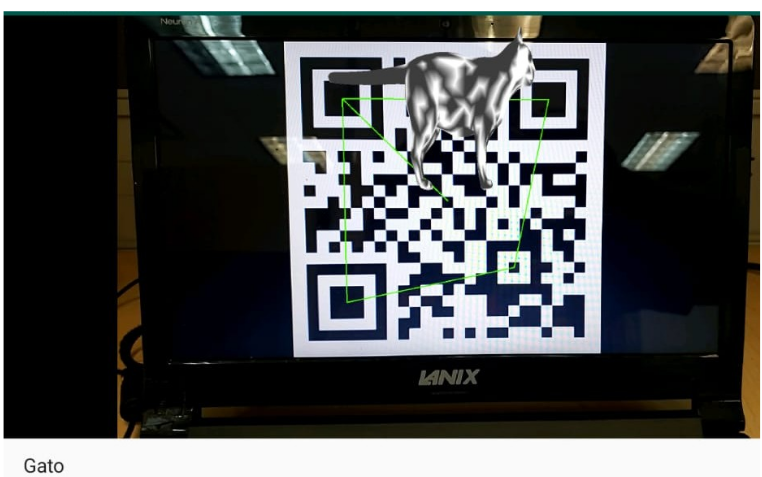
\includegraphics[width=0.98\textwidth]{Figs/SistemaAR3}\\
     \end{center}
\end{column}
\end{columns}



%\end{block} 
\end{frame}


\begin{frame}{Tutorial del uso de Blender \footnotemark}
%\begin{block}{Tutorial del uso de Blender \footnotemark} 
\begin{columns}
\begin{column}{0.23\textwidth}
    \begin{center}
	    \begin{tabular}{c}
		        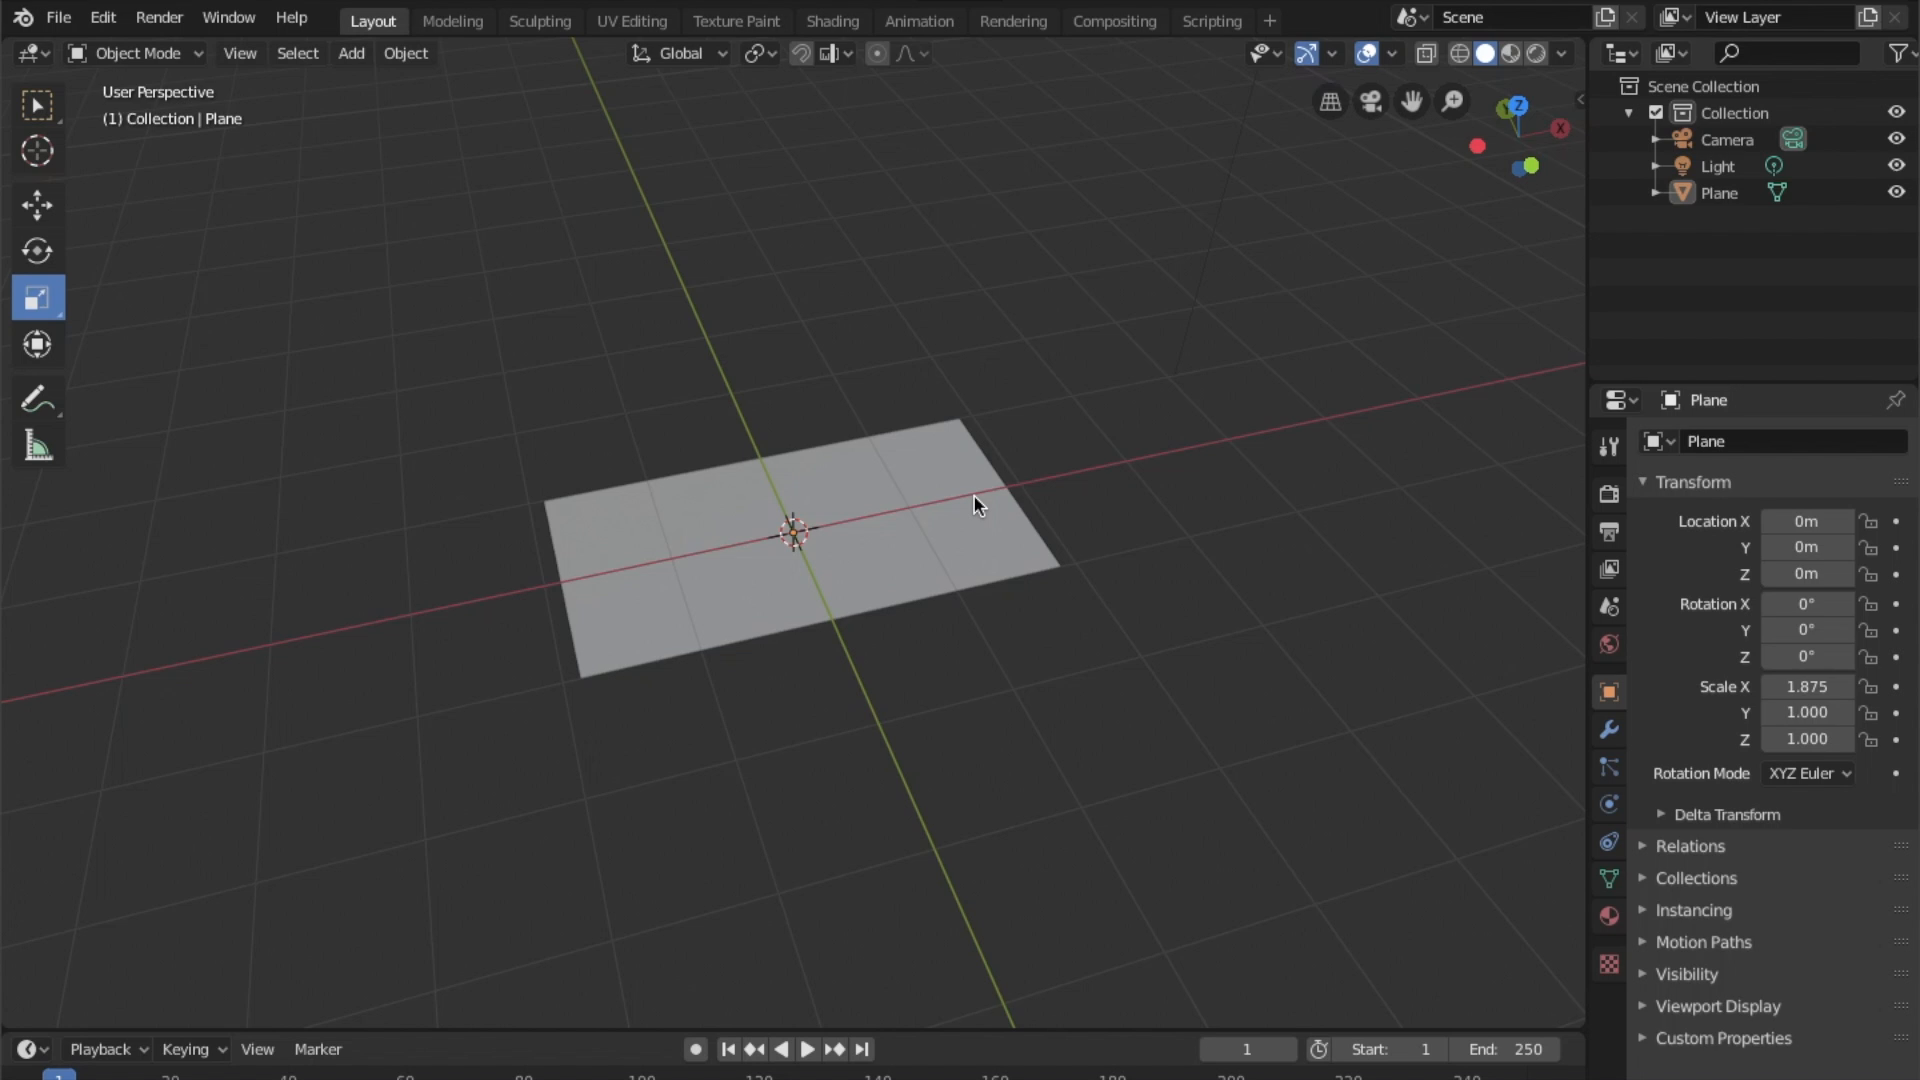
\includegraphics[width=0.75\linewidth]{Figs/VideoBlender01}\\
		        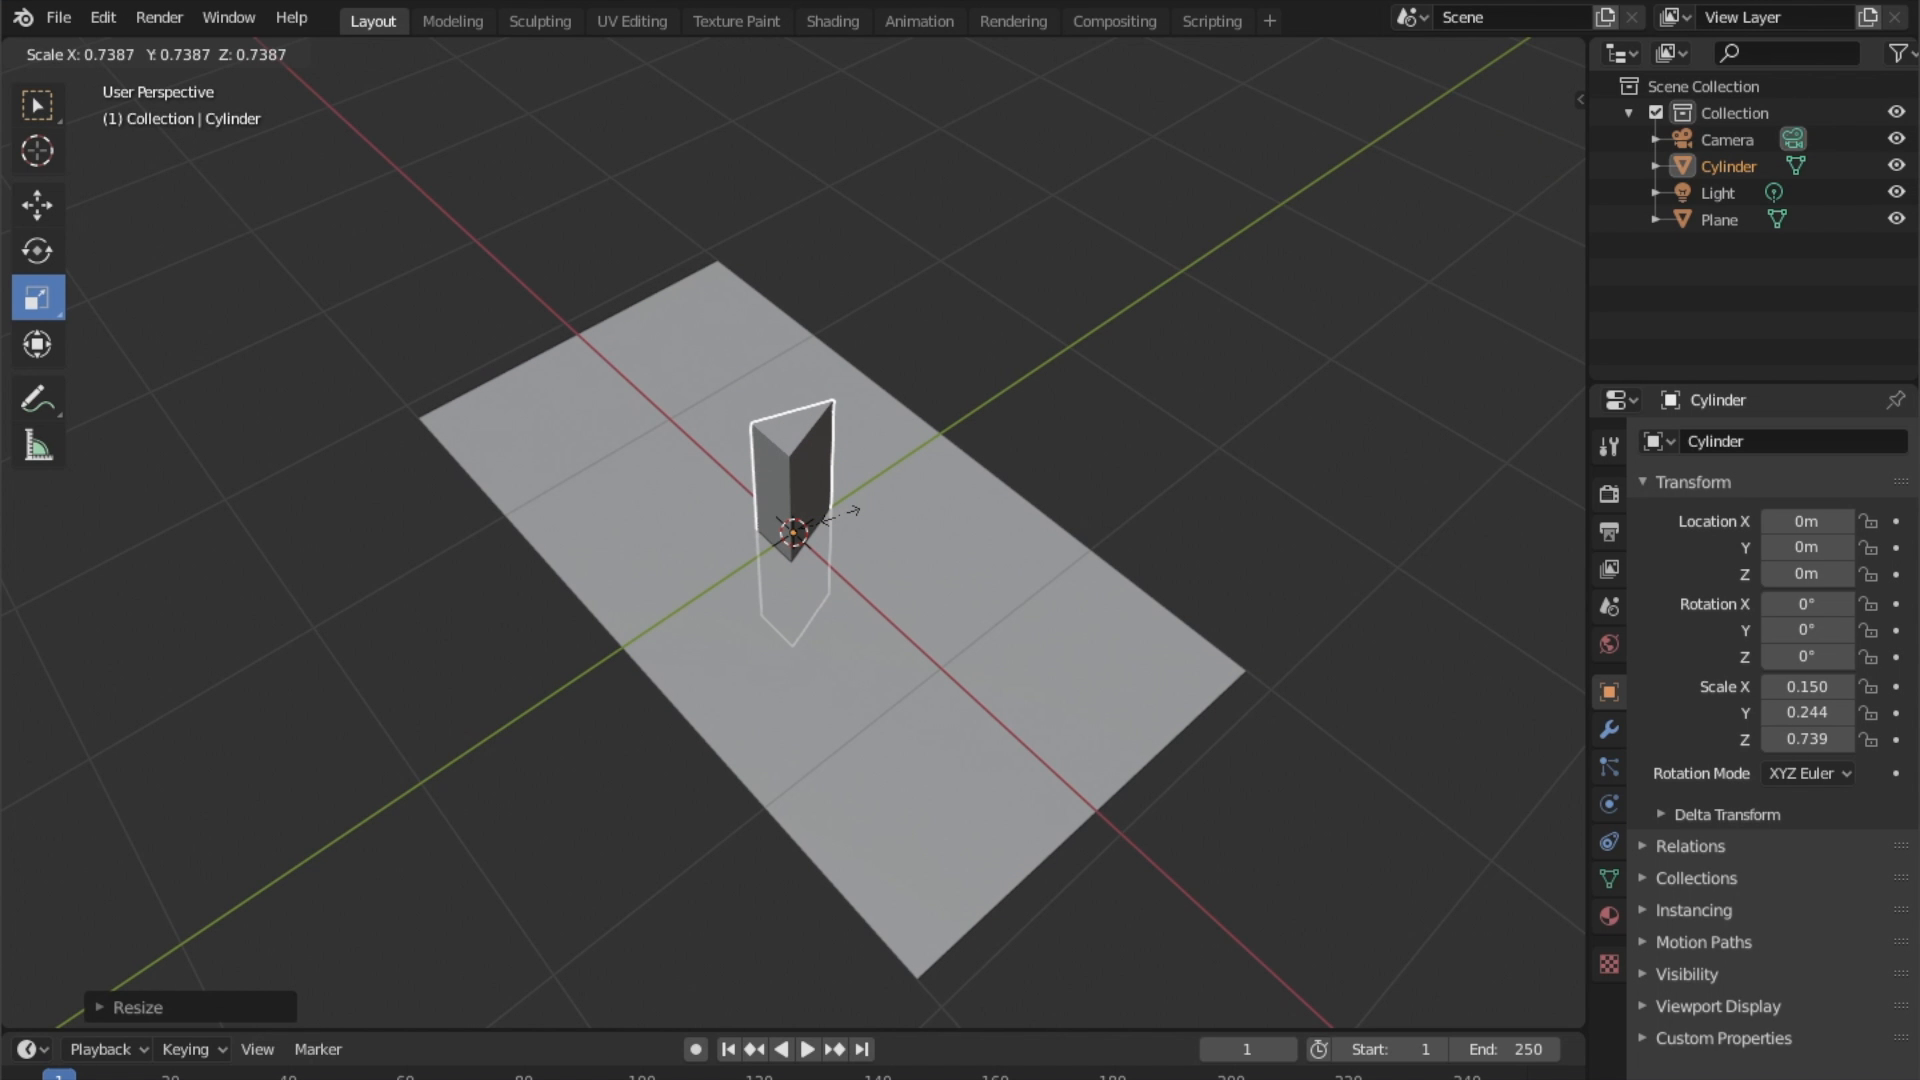
\includegraphics[width=0.75\linewidth]{Figs/VideoBlender02}\\
                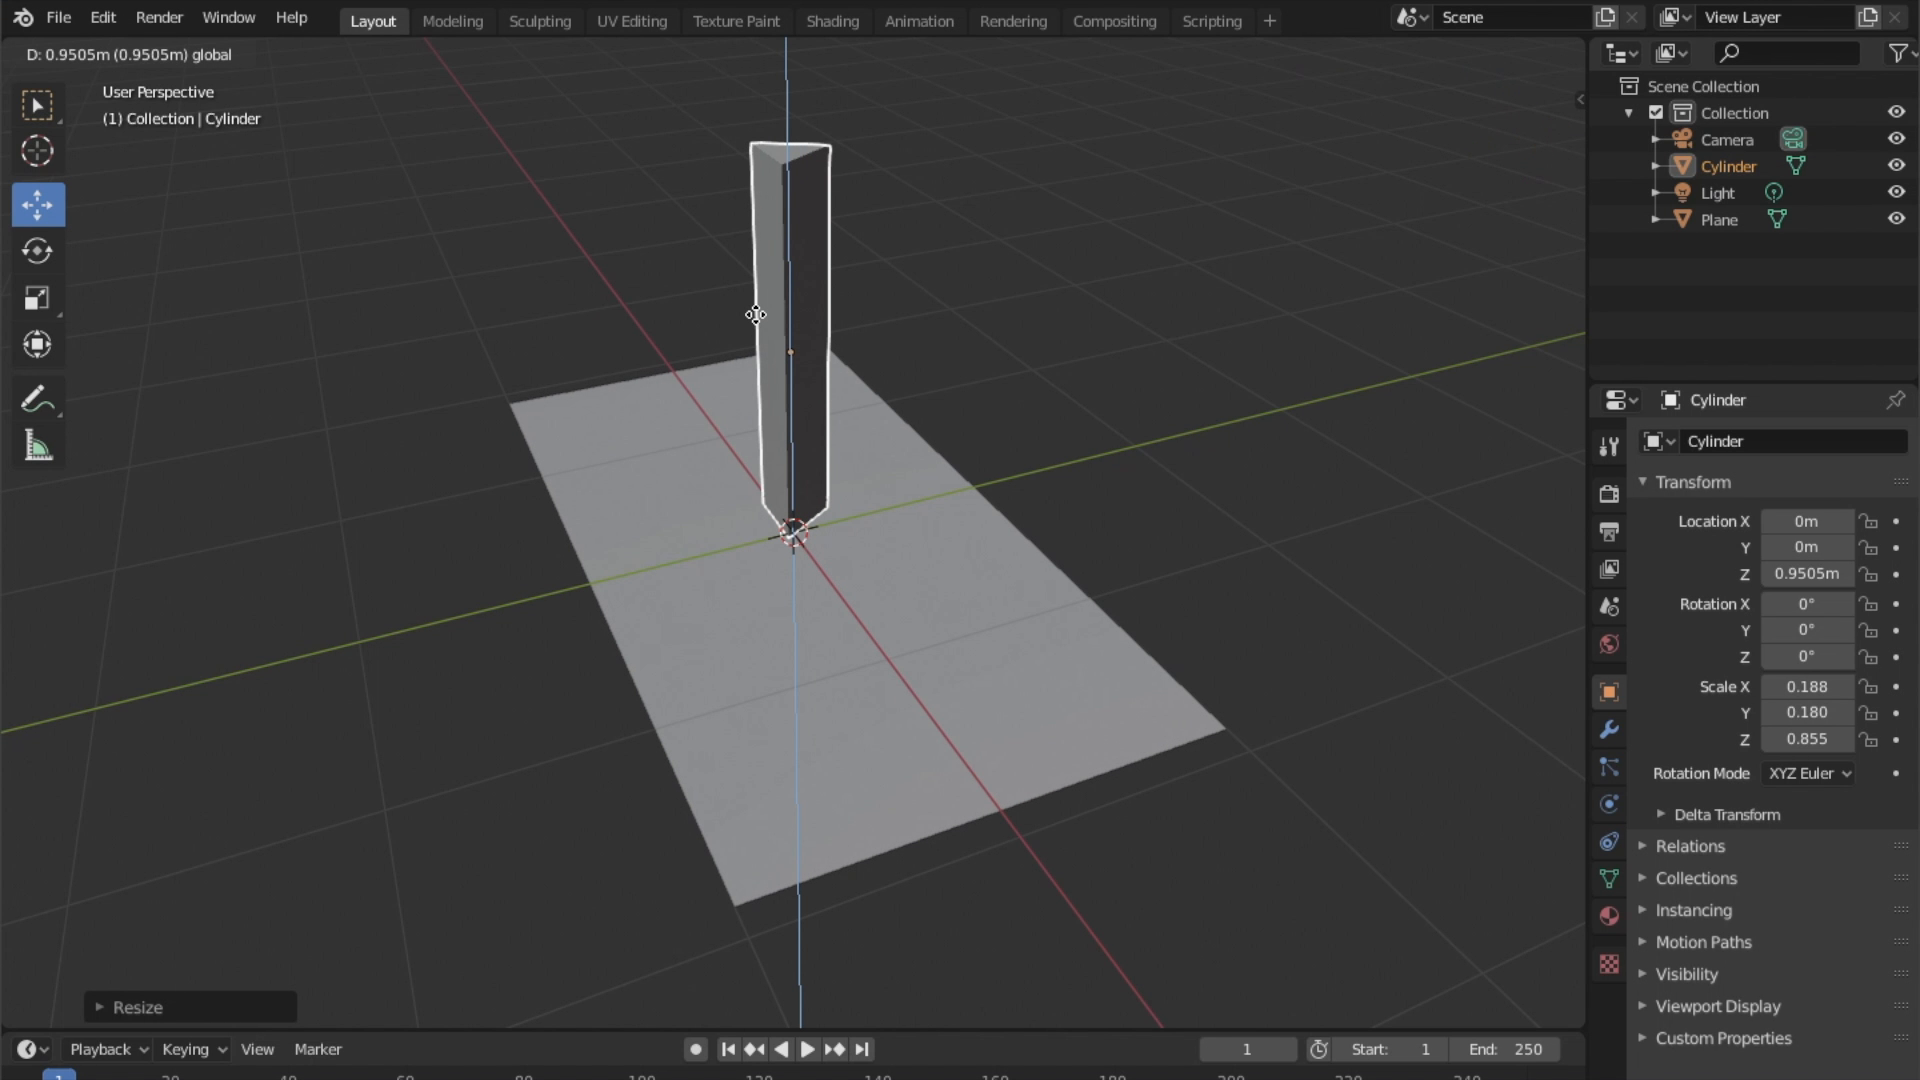
\includegraphics[width=0.75\linewidth]{Figs/VideoBlender03}\\
	    \end{tabular}
    \end{center}
\end{column}
\begin{column}{0.23\textwidth}
    \begin{center}
	    \begin{tabular}{c}
		        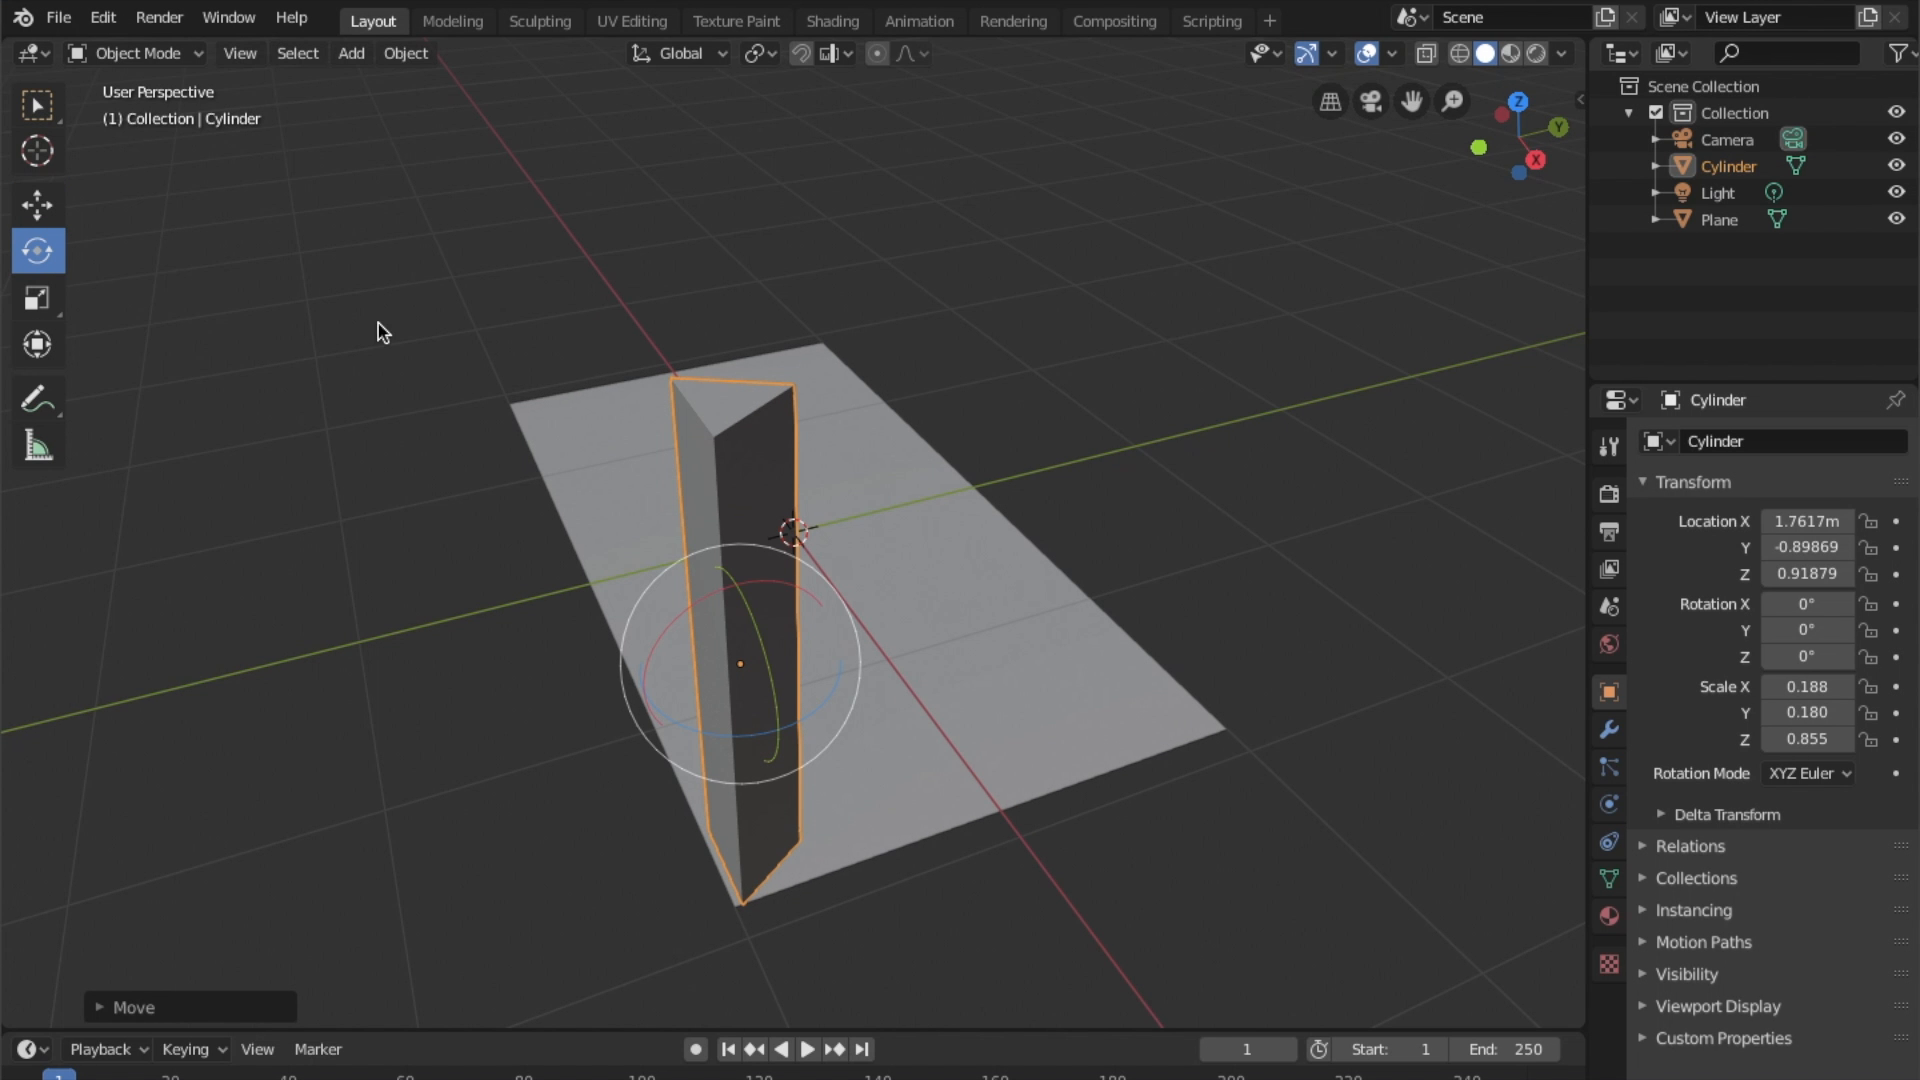
\includegraphics[width=0.75\linewidth]{Figs/VideoBlender04}\\
		        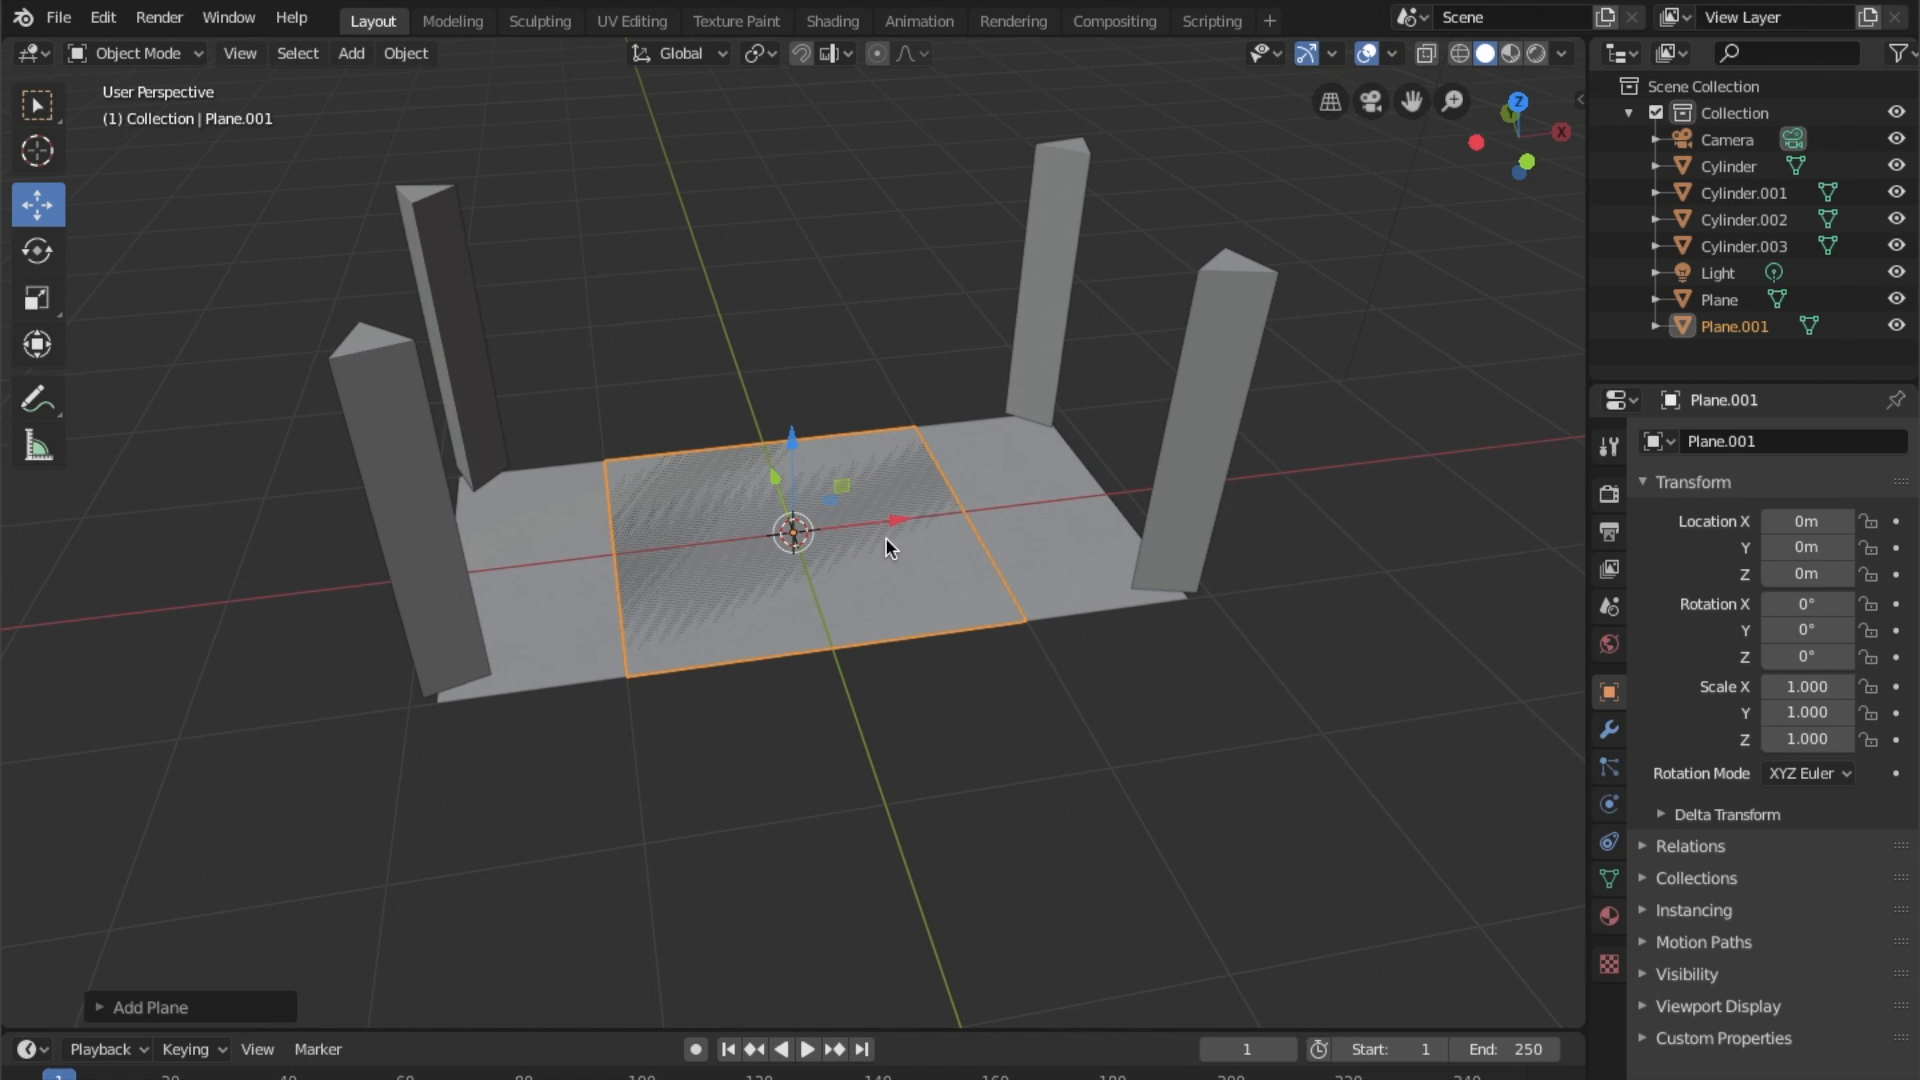
\includegraphics[width=0.75\linewidth]{Figs/VideoBlender05}\\
		        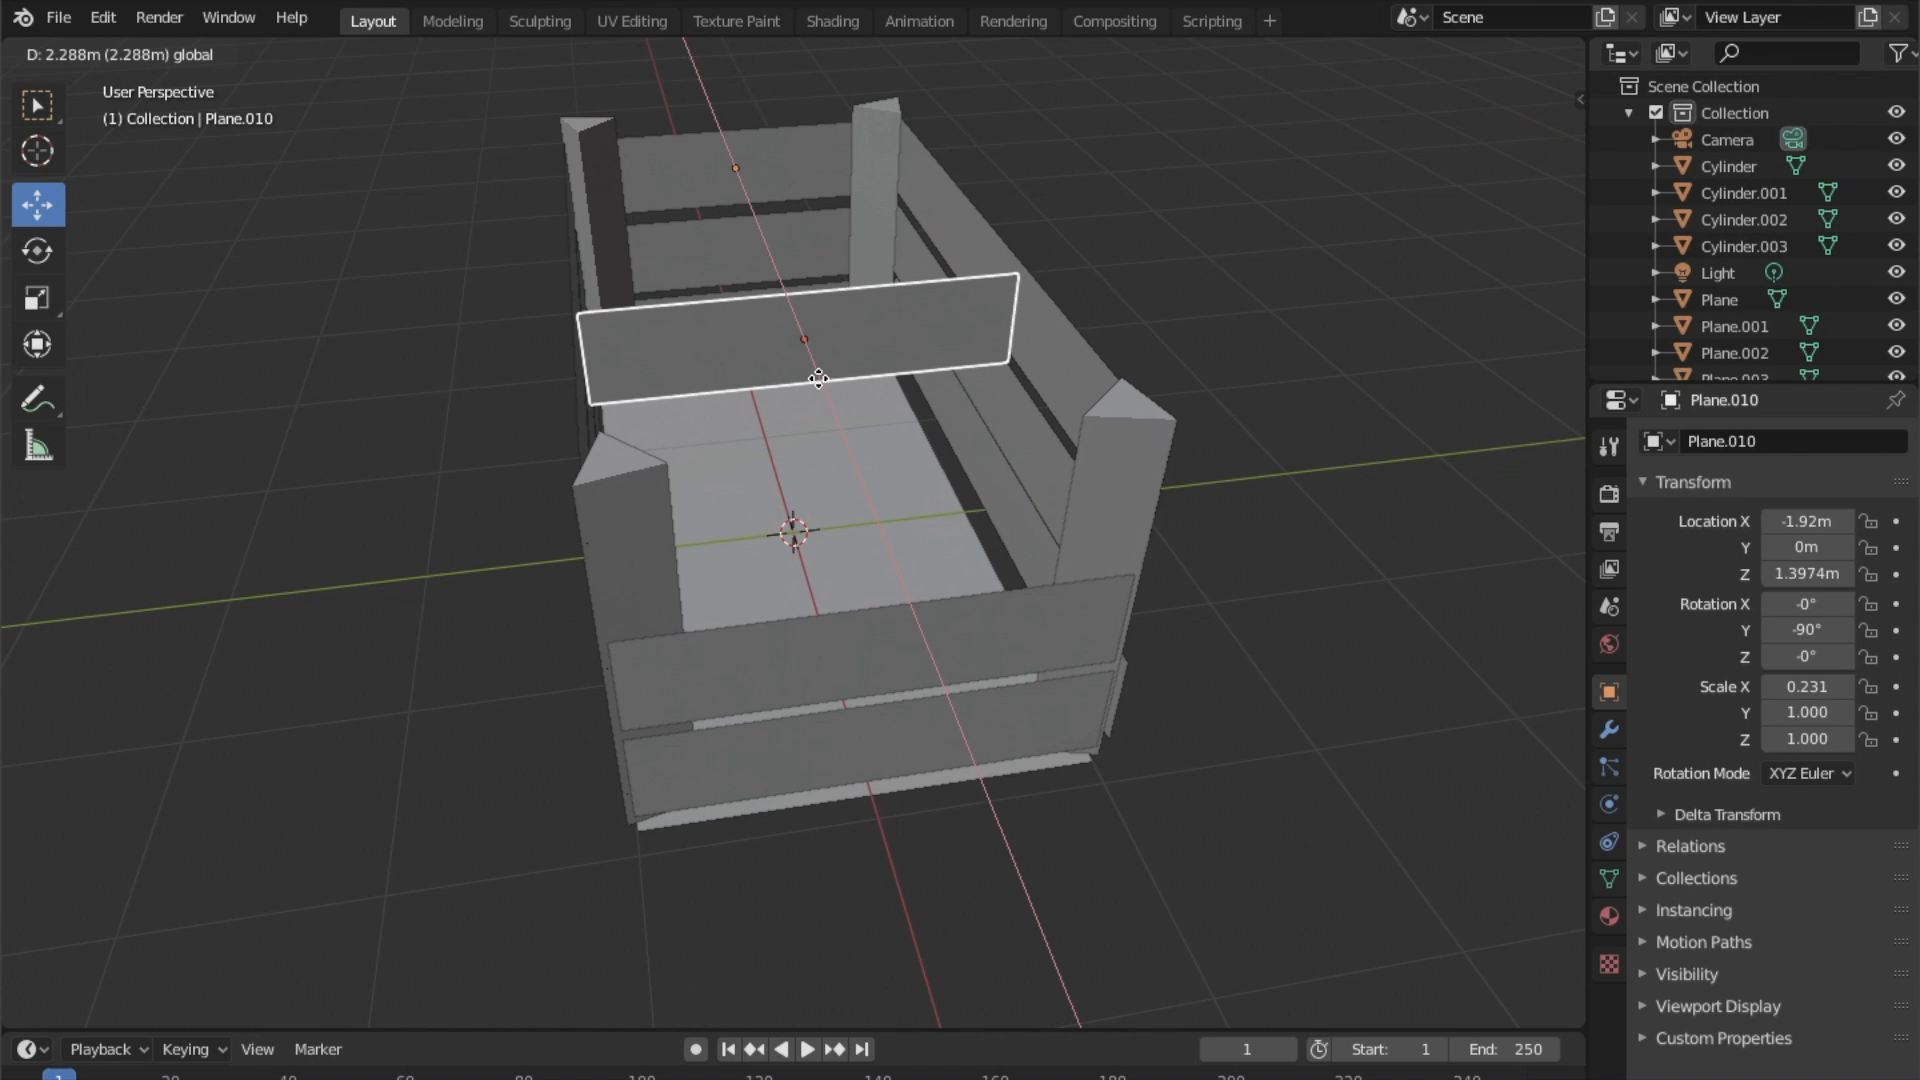
\includegraphics[width=0.75\linewidth]{Figs/VideoBlender06}\\
	    \end{tabular}
    \end{center}	
\end{column}
\begin{column}{0.23\textwidth}
    \begin{center}
	    \begin{tabular}{c}
		        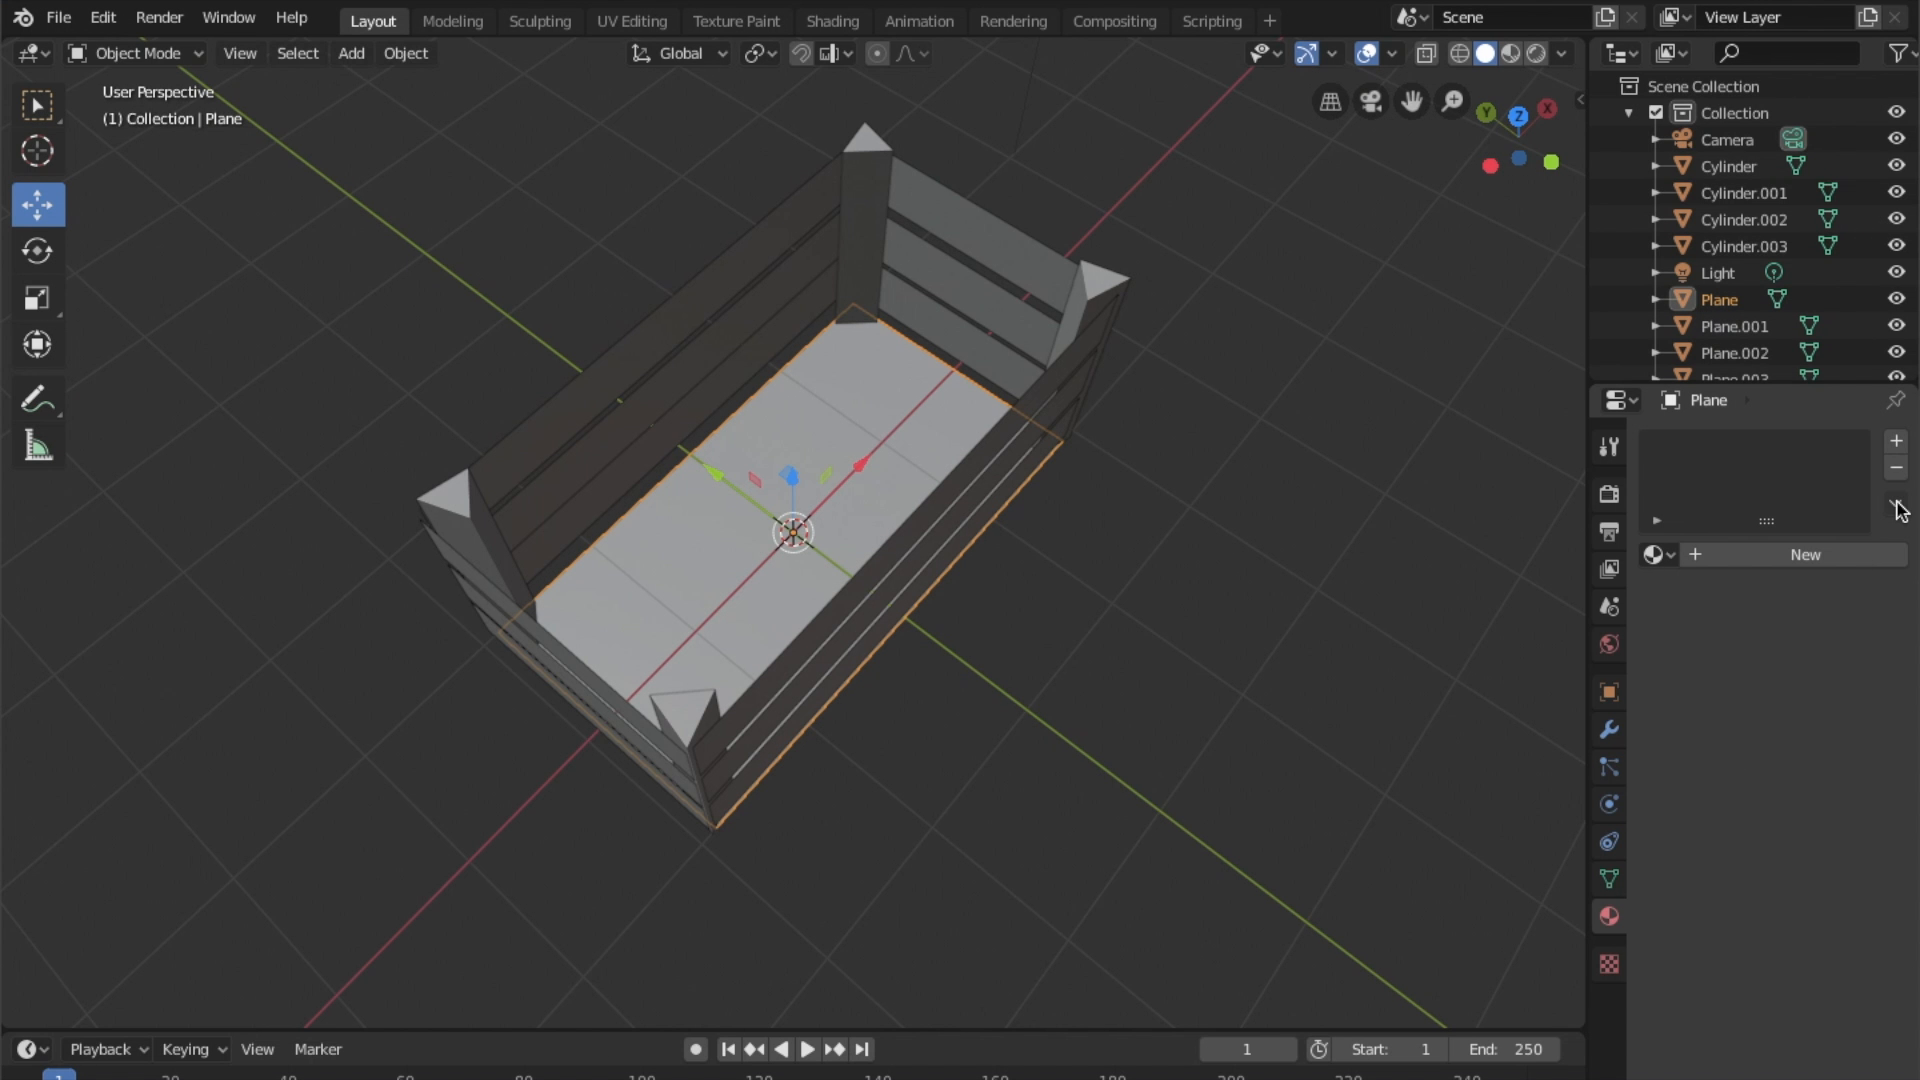
\includegraphics[width=0.75\linewidth]{Figs/VideoBlender07}\\
		        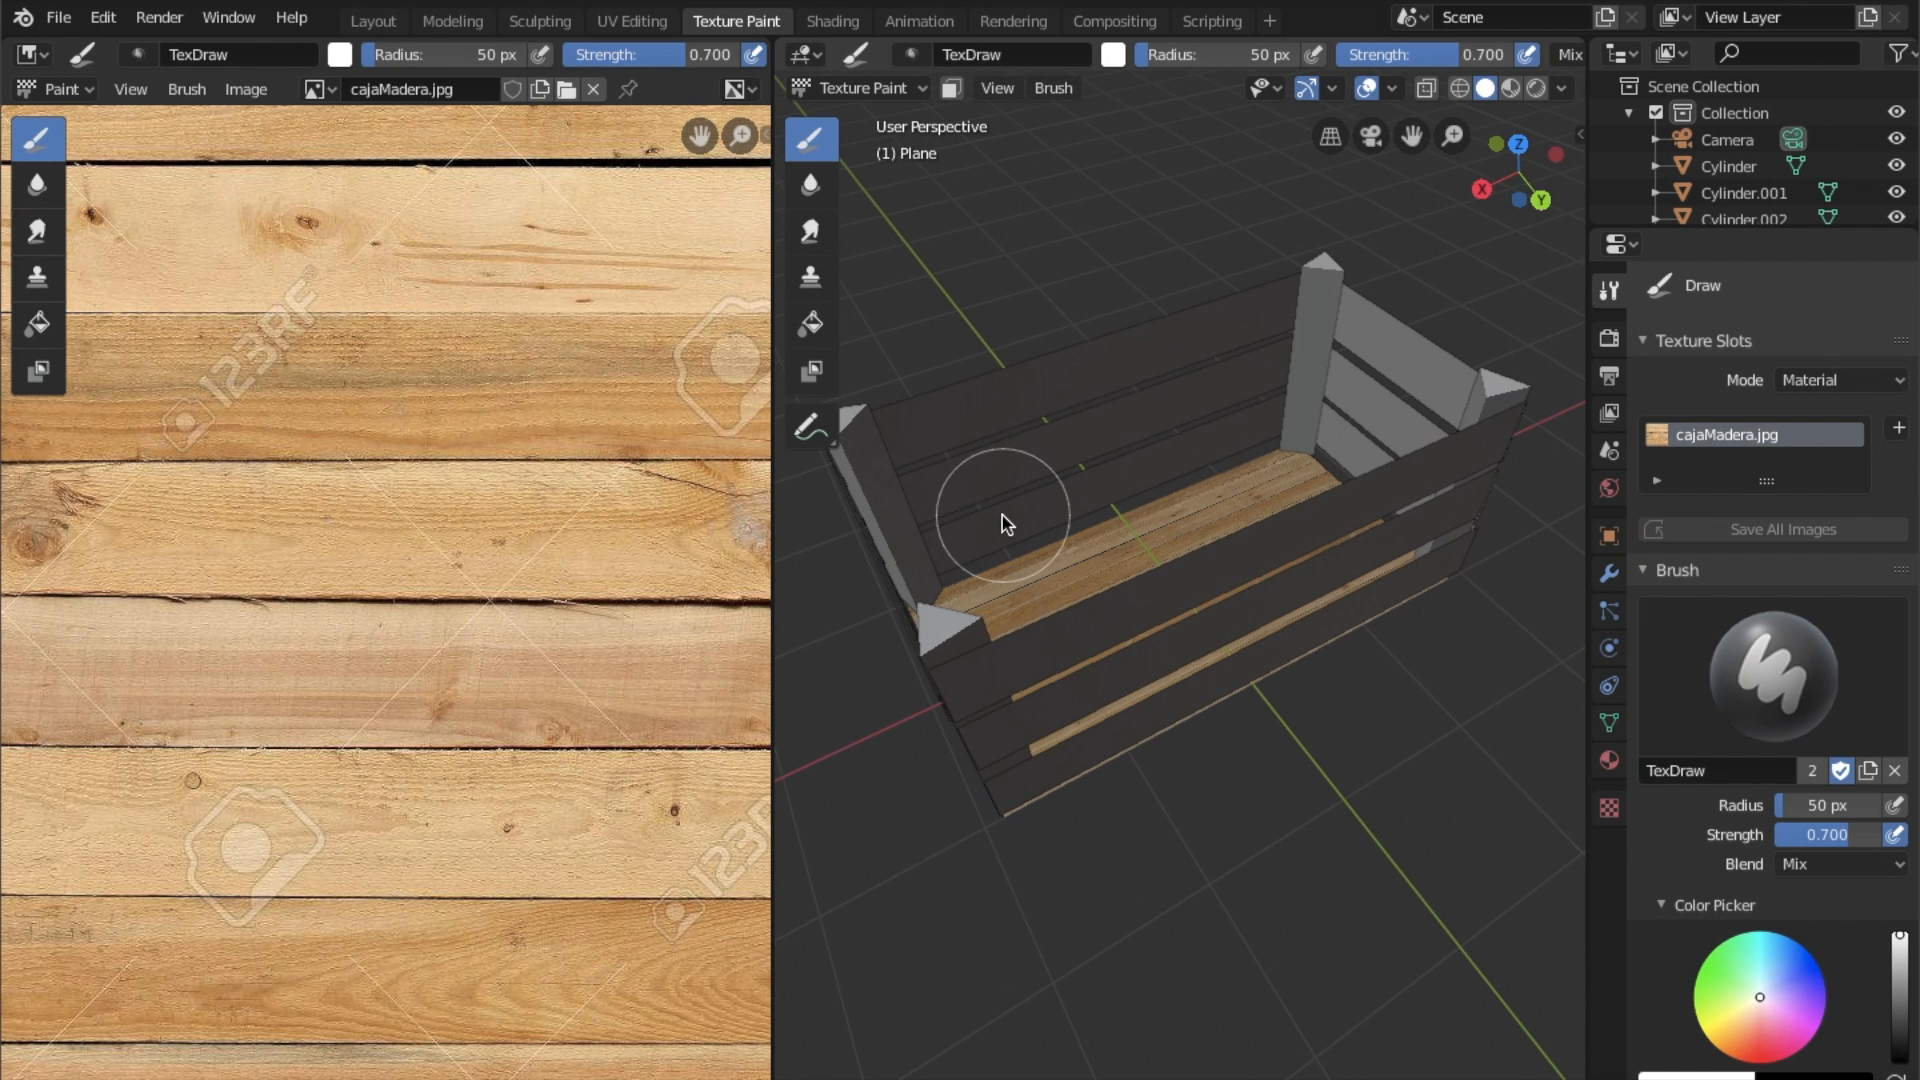
\includegraphics[width=0.75\linewidth]{Figs/VideoBlender08}\\
		        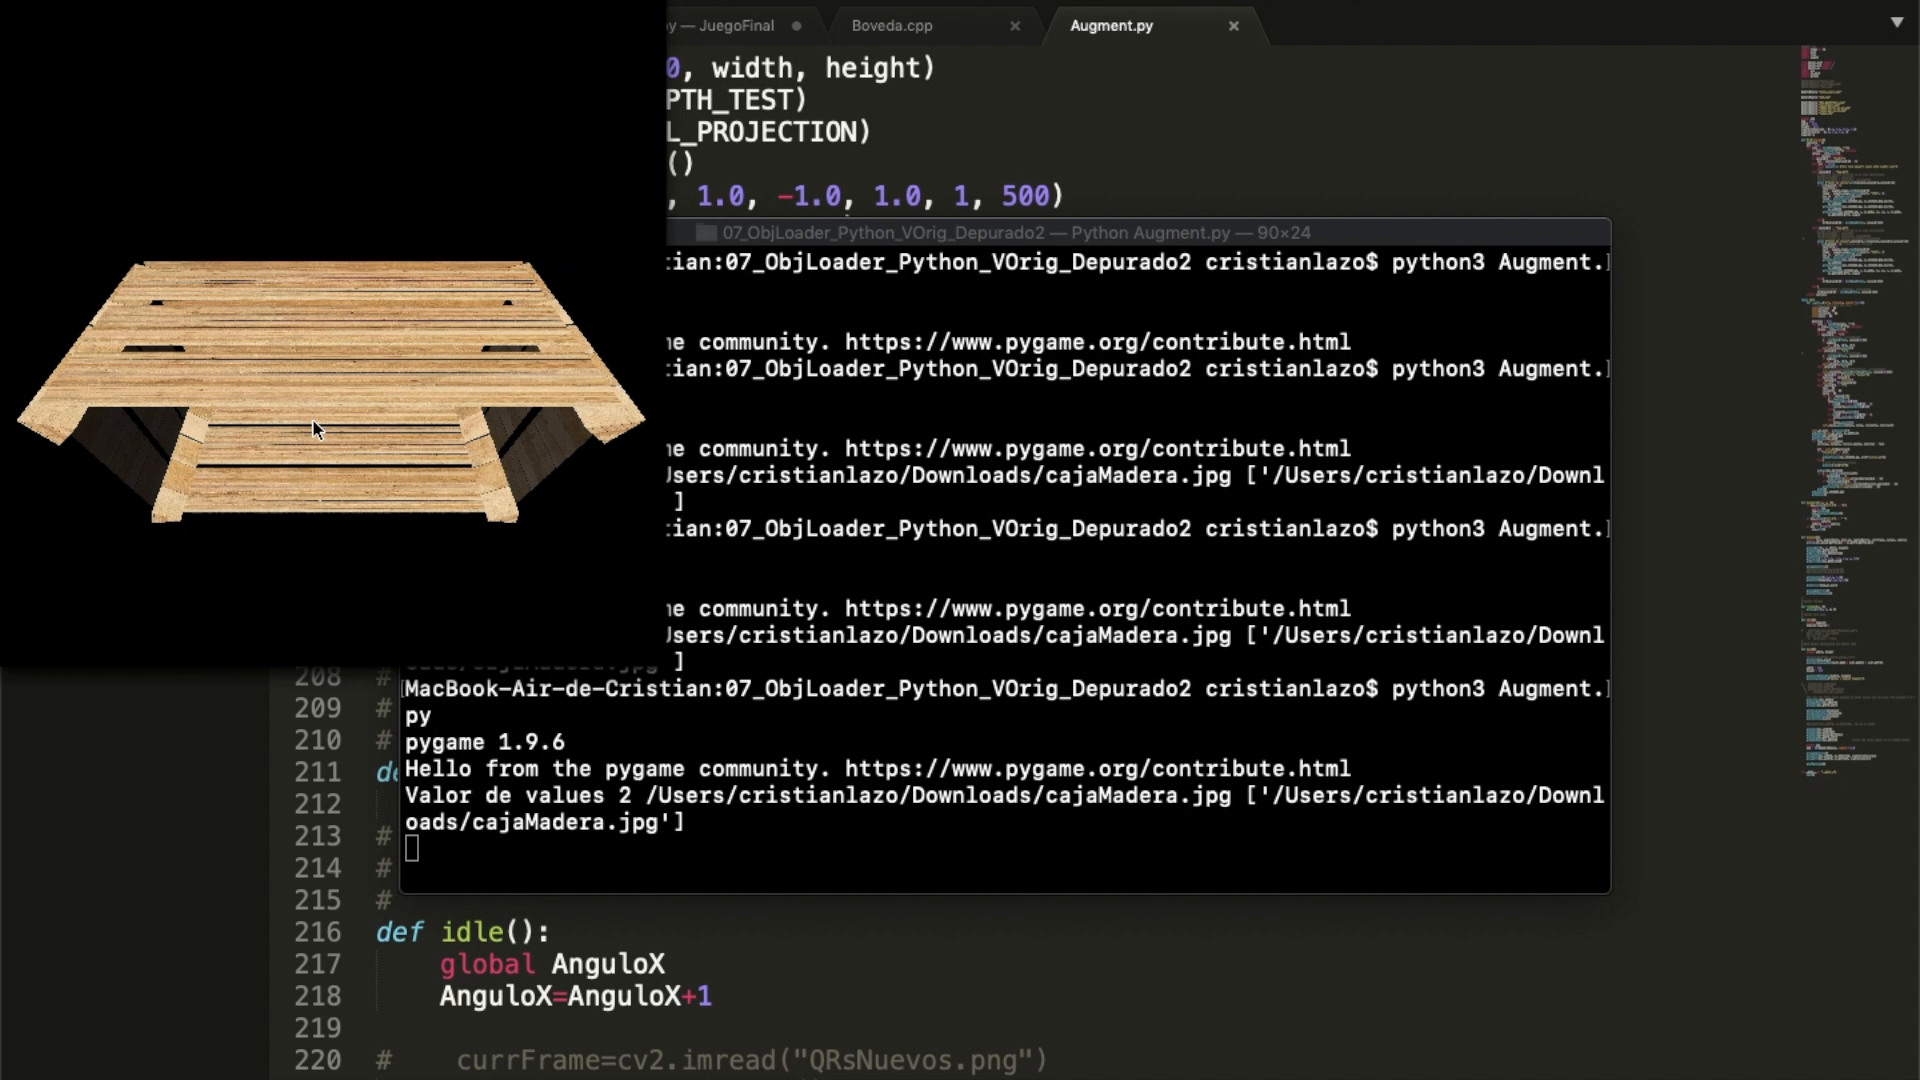
\includegraphics[width=0.75\linewidth]{Figs/VideoBlender09}\\
	    \end{tabular}
    \end{center}	
\end{column}
\begin{column}{0.23\textwidth}
    \begin{center}
	    \begin{tabular}{c}
		        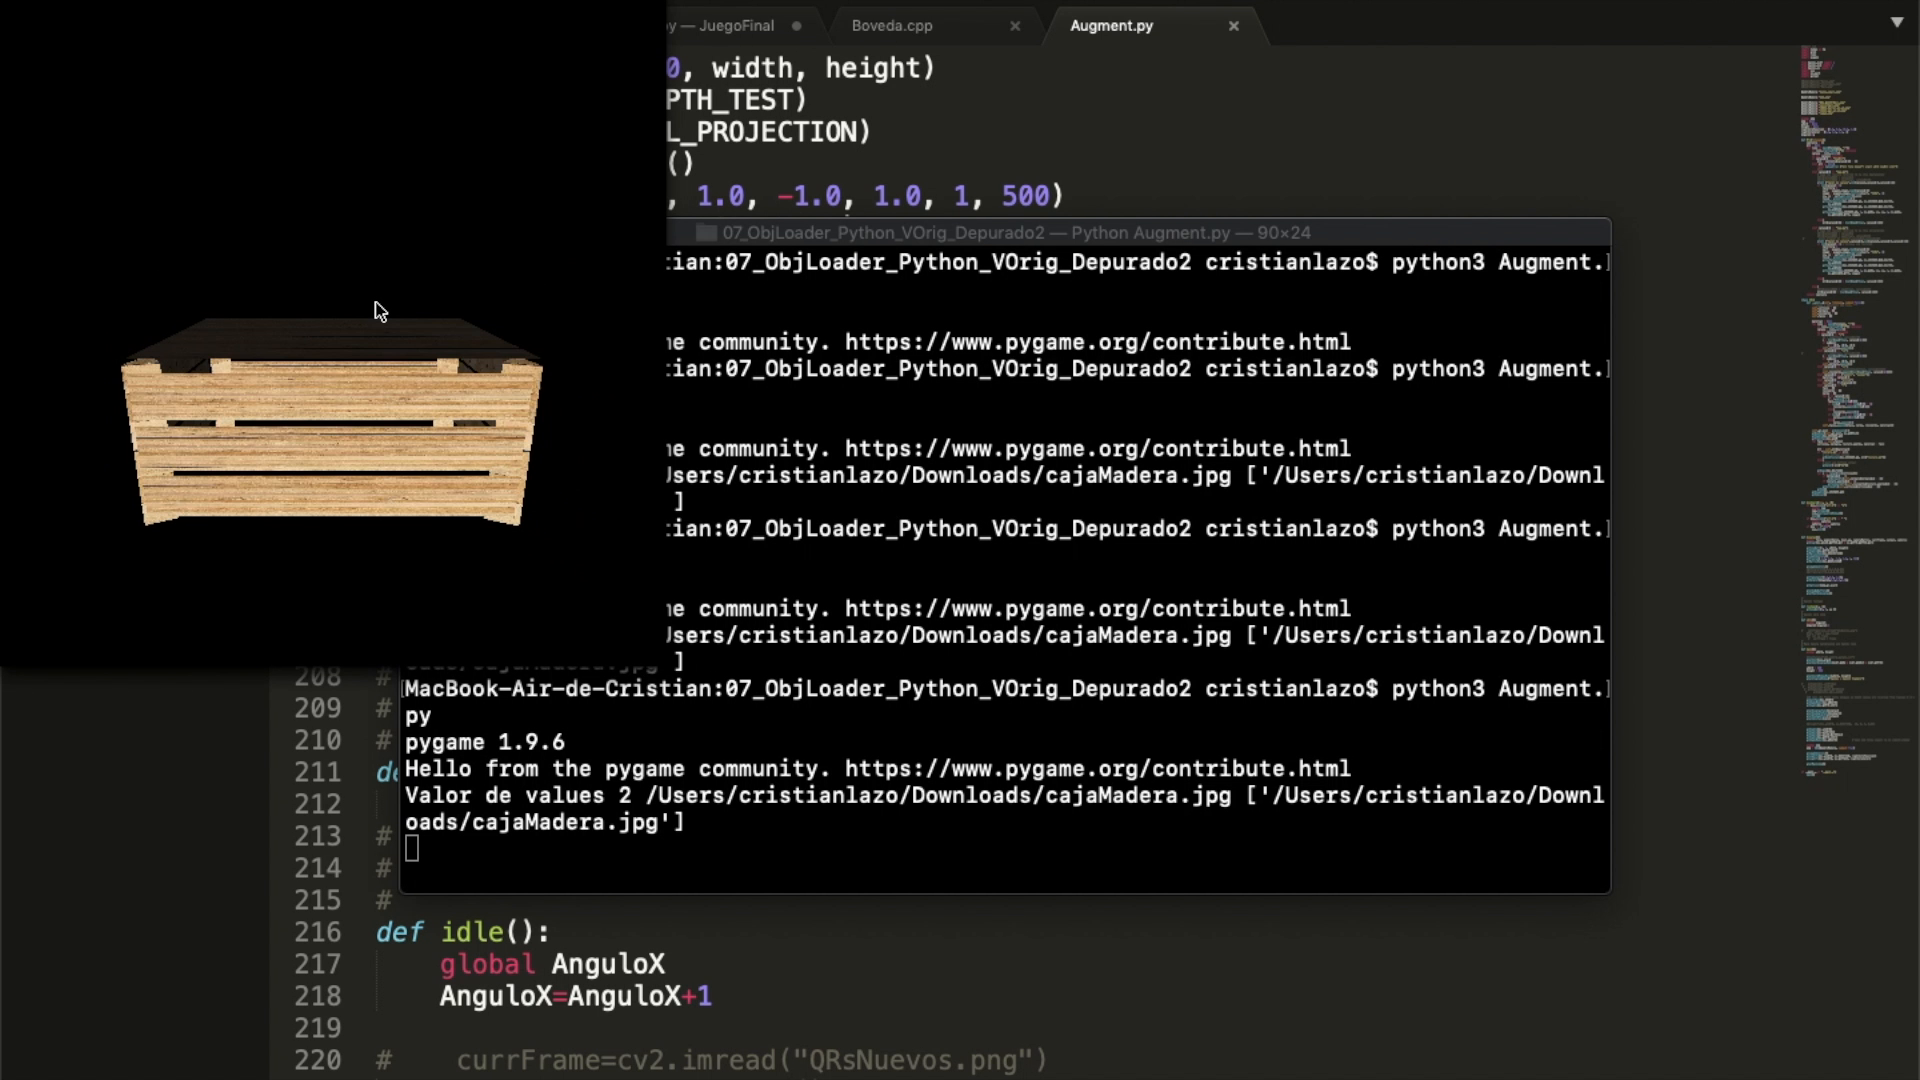
\includegraphics[width=0.75\linewidth]{Figs/VideoBlender10}\\
		        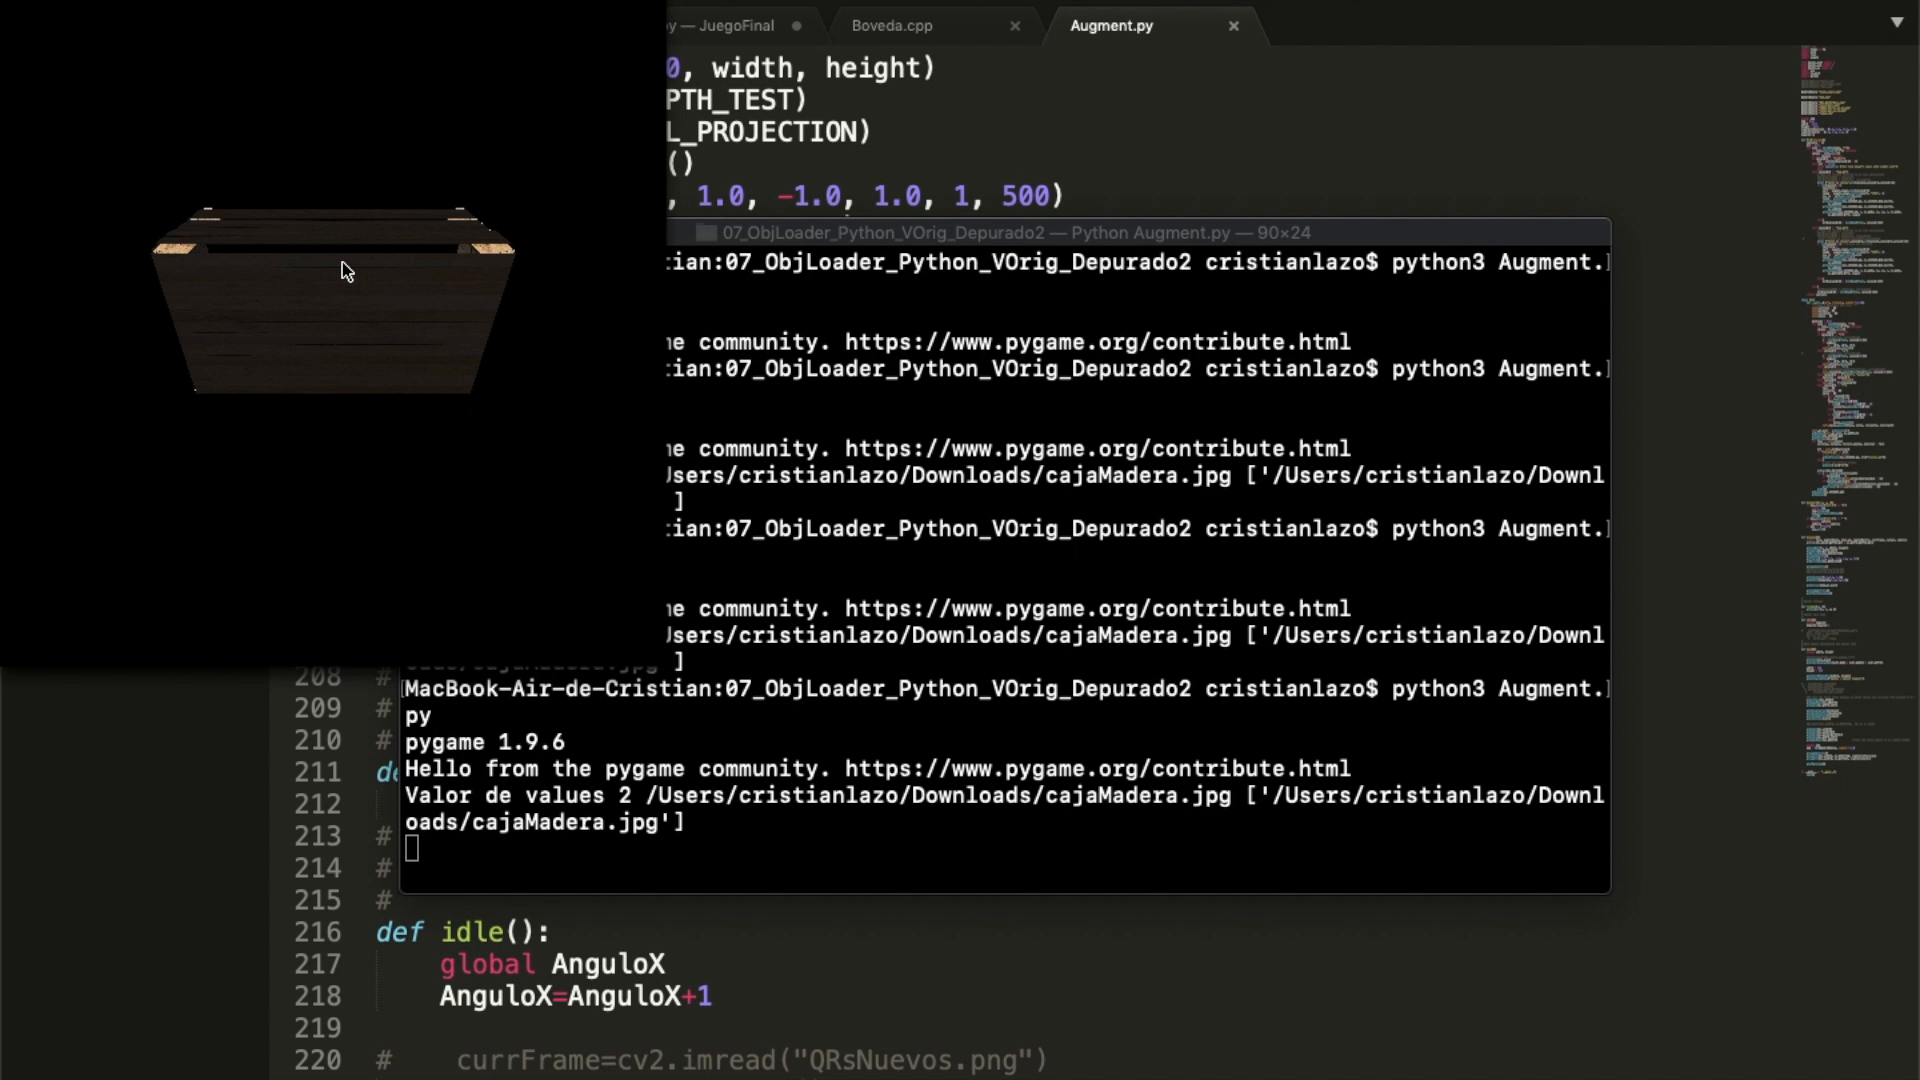
\includegraphics[width=0.75\linewidth]{Figs/VideoBlender11}\\
		        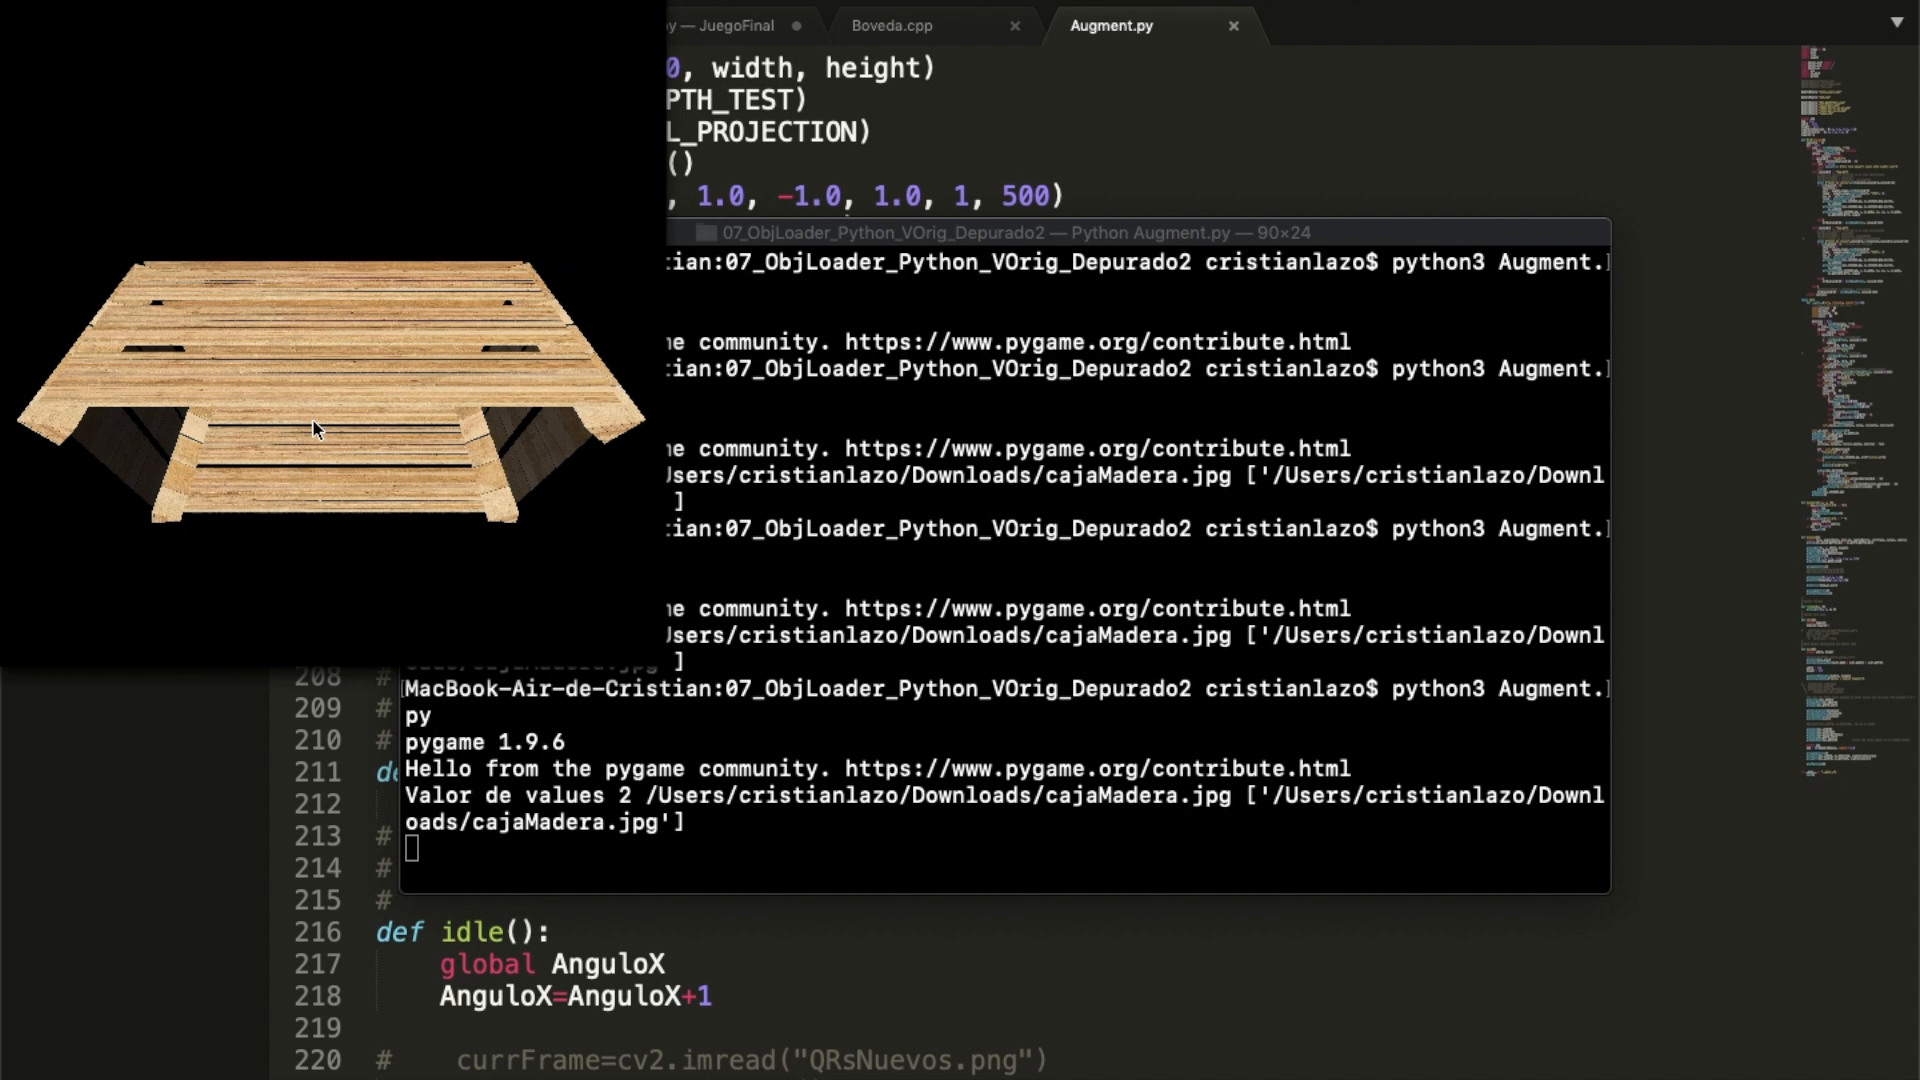
\includegraphics[width=0.75\linewidth]{Figs/VideoBlender12}\\
	    \end{tabular}
    \end{center}	
\end{column}

\end{columns}
%\end{block} 
\footnotetext{\fullcite{TutorialBlender_Lazo_2020}}
\end{frame}


\begin{frame}{Detección de movimientos en un tablero de ajedrez \footnotemark}
%\begin{block}{Detección de movimientos en un tablero de ajedrez \footnotemark} 
\begin{columns}
\begin{column}{0.38\textwidth}
Aplicación de escritorio:
	\begin{itemize}
\item Entorno semicontrolado con una cámara y una Laptop con OpenCV
\item Detecta las esquinas del tablero de ajedrez
\item Transformada de Hough
\item Detectar si hay casilla o no dentro de la región de interés
	\end{itemize}
\end{column}
\begin{column}{0.28\textwidth}
\begin{center}
     %%%%% this is a minipage, so \textwidth is already adjusted to the size of the column
     \includegraphics[width=0.75\textwidth]{Figs/AjedrezFroylan1}\\
%     \includegraphics[width=0.35\textwidth]{Figs/AjedrezFroylan2}
     \end{center}
\end{column}
\begin{column}{0.28\textwidth}
\begin{center}
     %%%%% this is a minipage, so \textwidth is already adjusted to the size of the column
 %    \includegraphics[width=0.35\textwidth]{Figs/AjedrezFroylan1}\\
     \includegraphics[width=0.75\textwidth]{Figs/AjedrezFroylan2}
     \end{center}
\end{column}

\end{columns}
%\end{block} 
\footnotetext{\fullcite{Froylan_VC_2021}}
%\footnotetext{Froylan Melquiades Wbario Martinez, \textbf{Seguidor de movimientos de Ajedrez}. Universidad Politécnica de Victoria, Informe técnico proyecto de asignatura “Visión por Computadora”, 2021.  En evaluación.}
%\\setcounter{footnote}{0}
\end{frame}

\begin{frame}{Detección de movimientos en un tablero de ajedrez (2)}
%\begin{block}{Detección de movimientos en un tablero de ajedrez (2)} 
\begin{columns}
\begin{column}{0.38\textwidth}
Aplicación de escritorio:
	\begin{itemize}
\item Una vez detectadas las regiones, se emplea un cronometro para determinar la diferencia entre dos instantaneas consecutivas
\item Problemas actuales: Iluminación, sombras, oclusiones
	\end{itemize}
\end{column}
\begin{column}{0.28\textwidth}
\begin{center}
     %%%%% this is a minipage, so \textwidth is already adjusted to the size of the column
     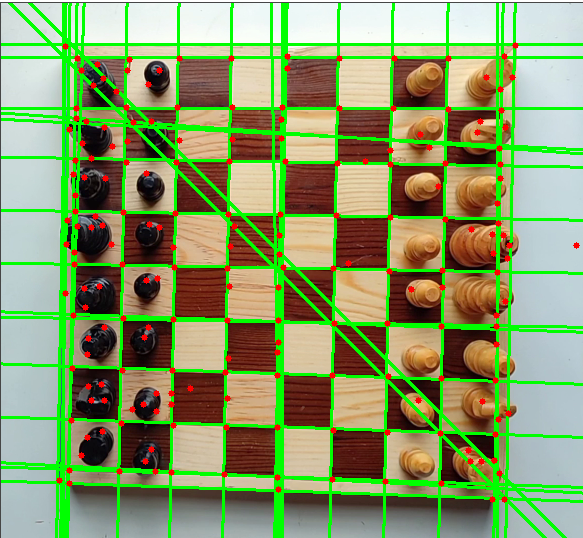
\includegraphics[width=0.79\textwidth]{Figs/AjedrezFroylan3}\\
%     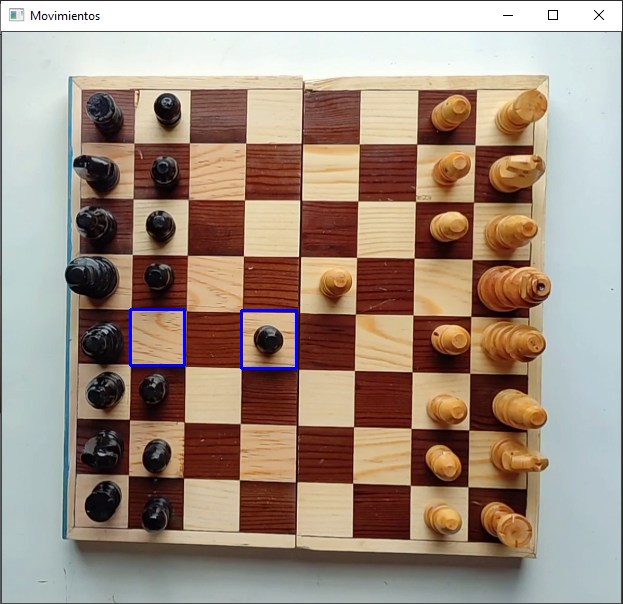
\includegraphics[width=0.49\textwidth]{Figs/AjedrezFroylan4}
     \end{center}
\end{column}
\begin{column}{0.28\textwidth}
\begin{center}
     %%%%% this is a minipage, so \textwidth is already adjusted to the size of the column
%     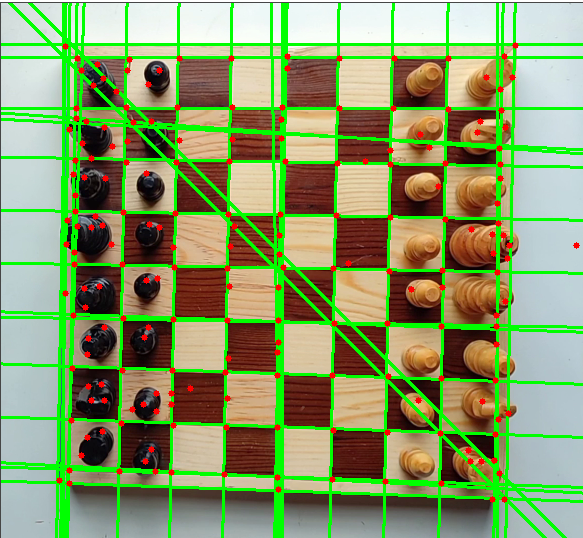
\includegraphics[width=0.49\textwidth]{Figs/AjedrezFroylan3}\\
     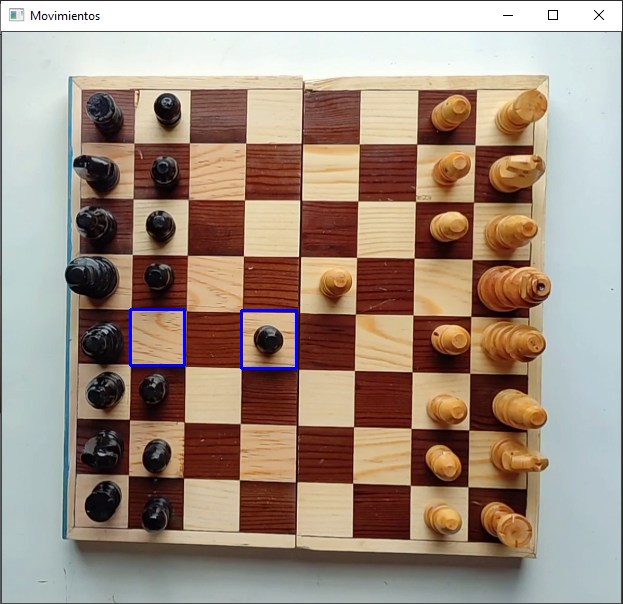
\includegraphics[width=0.79\textwidth]{Figs/AjedrezFroylan4}
     \end{center}
\end{column}

\end{columns}
%\end{block} 
\end{frame}



\end{document}

\section{Introduccion}
\subsection{IA, ML, VC y GC}
\begin{frame}{Inteligencia Artificial}
%\Huge

		\begin{columns}
		\begin{column}{0.57\textwidth}
		\begin{itemize}
		\item Es un subconjunto de las ciencias de la computación (CC) en donde las máquinas aparentan inteligencia mediante la ejecución de programas. 
		\item Las computadoras intentan resolver tareas que solo son posibles mediante inteligencia humana.
		\item Es una rama muy amplia que cubre muchos aspectos de la vida cotidiana.
		\end{itemize}
		\end{column}
		\begin{column}{0.37\textwidth}  
			\begin{center}
			 %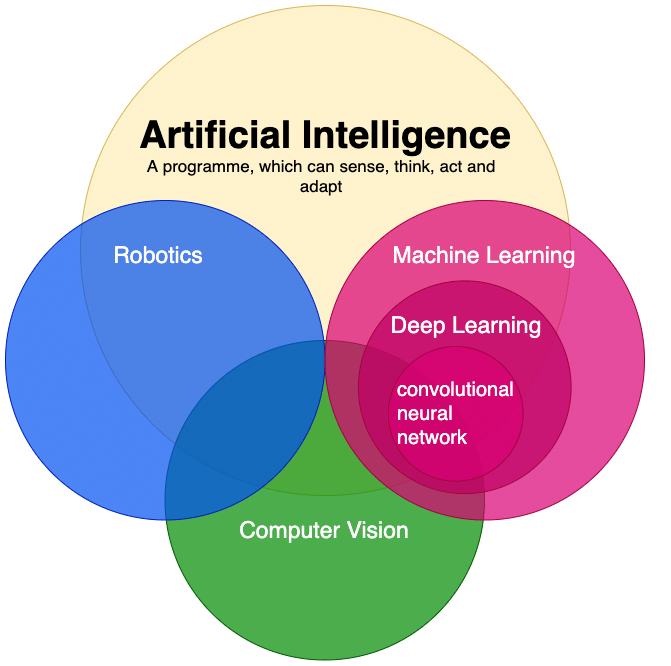
\includegraphics[width=\textwidth]{Figs/Ai1}
\resizebox{\columnwidth}{!}{%
				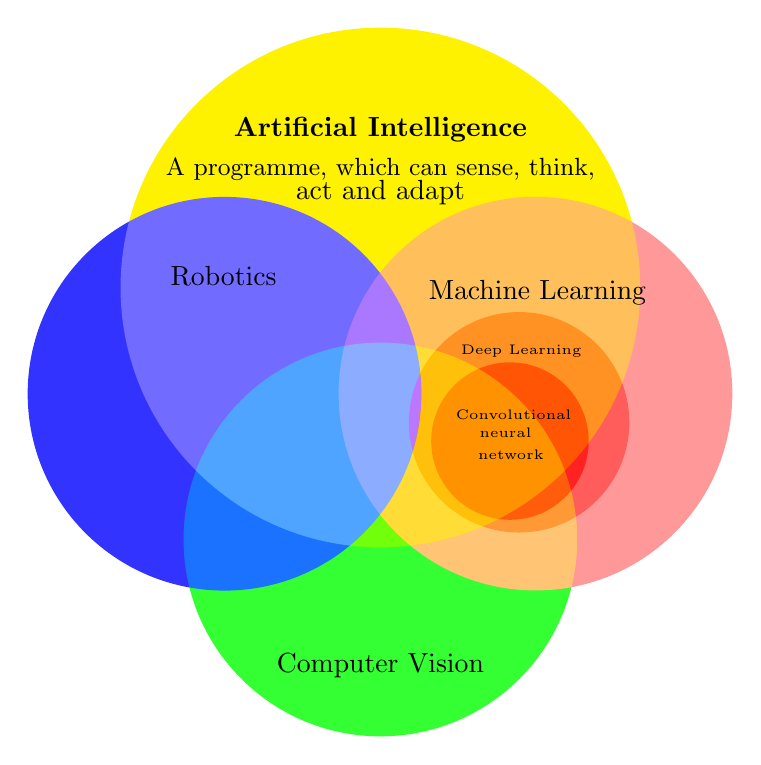
\begin{tikzpicture}
				  \begin{scope}[blend group = soft light]
					\fill[blue!80] (190:2.01) circle (2.5);
					\fill[red!40]  (350:2) circle (2.5);
					\fill[green!80]   ( -90:2.2) circle (2.5);
					\fill[red!100]  (338:1.9) circle (1.4);
					\fill[black!100]  (330:1.9) circle (1);
					\fill[yellow!100]   ( 90:1) circle (3.3);
				   
				   
				  \end{scope}
				  \node at ( 90:3)      {\textbf{Artificial Intelligence}};
				  \node at ( 90:2.5)    {\small A programme, which can sense, think,};
				  \node at ( 90:2.2)    {act and adapt};
				  \node at ( 150:2.3)   {Robotics};
				  \node at ( 385:2.2)   {Machine Learning};
				  \node at ( 366:1.8)   {\tiny Deep Learning};
				  \node at ( 340:1.8)   {\tiny Convolutional};
				  \node at ( 332:1.8)   {\tiny neural};
				  \node at ( 326:2.0)   {\tiny network};
				  \node at ( -90:3.8)   {Computer Vision};
				\end{tikzpicture}
}

			 \end{center}
		\end{column}
	\end{columns}

\end{frame}



\begin{frame}{Visión por Computadora}
%\begin{block}{Fundamentación} 
\begin{columns}
\begin{column}{0.60\textwidth}
    \begin{center}
\begin{itemize}
\item La visión por computadora imita la percepción humana y las capacidades de razonamiento.
\item Se intenta inferir conocimiento a partir de imágenes o videos.
\item Procesamiento de imágenes es una fase temprana de la VC. La entrada es una imagen y la salida es otra imagen.
\item En la visión por computadora, la entrada es una imagen pero la salida son datos. 
\end{itemize}
     \end{center}

\end{column}
\begin{column}{0.40\textwidth}  
    \begin{center}
     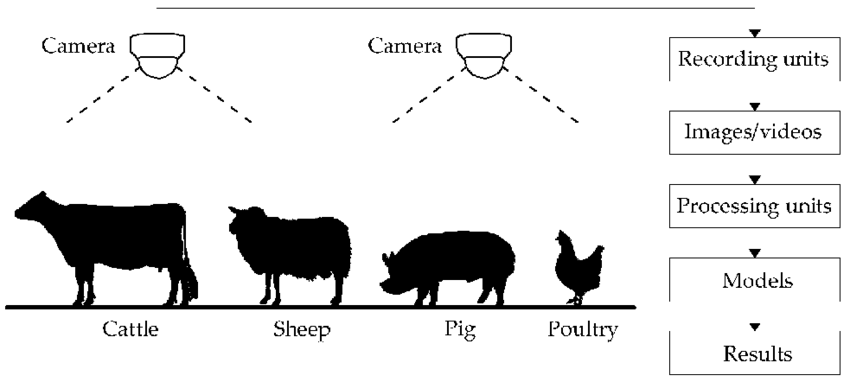
\includegraphics[width=0.9\textwidth]{Figs/VC}
     \end{center}
\end{column}
\end{columns}
%\end{block} 
\end{frame}

\begin{frame}{Visión por Computadora (Detección de Bordes) (II)}
  \begin{columns}
  \column {0.4\textwidth}
  \begin{itemize}
    \item La información acerca de bordes es útil para entender el ambiente.
    \item Las esquinas son primitivas que permiten identificar limites y puntos de interés dentro de la geometría de las imágenes.
  \end{itemize}  
      \column {0.3\textwidth}  
        \begin{center}
            \includegraphics[width=\textwidth]{Figs/VC_CocaOrig}\\
     \end{center}
      
    \column {0.3\textwidth}  
        \begin{center}
            \includegraphics[width=\textwidth]{Figs/VC_CocaBordes}
     \end{center}

    \end{columns}

\end{frame}

\begin{frame}{Visión por Computadora (Segmentación) (II)}
\begin{columns}
  \column {0.8\textwidth}
  \begin{itemize}
    \item Localizar y aislar objetos de interés en la imagen.
    \item Localización de Objetivos, navegación, conteo de objetos
    \item Algoritmos de segmentación en escala de grises. Segmentación global (un umbral común para toda la imagen y segmentación local (umbrales múltiples en regiones de la imágen).
    \item Algoritmos de segmentación por color: muy utilizados para detectar la piel y encontrar partes del cuerpo.
  \end{itemize}
  
    \column {0.2\textwidth}  
        \begin{center}
            \includegraphics[width=\textwidth]{Figs/VC_Segmentacion}\\
     \end{center}

    \end{columns}
\end{frame}

\begin{frame}{Visión por Computadora (Template Matching) (II)}

Permite comparar imágenes aplicando operaciones de comparación entre regiones.
\begin{columns}
  \column {0.5\textwidth}
  \begin{itemize}
    \item Algoritmos clásicos basados en correlación: SAD, SSD, Rank.
	  \begin{itemize}
		    \item Ventajas: Facil de entender, rápidos
		    \item Desventajas: Sensibles a la escala, a rotaciones y a cambios en la iluminación. 
	  \end{itemize}
    \item Algoritmos modernos basados Aprendizaje Profundo
		\begin{itemize}
		    \item Ventajas: Buen desempeño 
		    \item Desventajas: Requieren de entrenamiento con muchas imágenes
	  \end{itemize}

  \end{itemize}
    \column {0.5\textwidth}  
        \begin{center}
            \includegraphics[width=\textwidth]{00_IntroComputerVision/figs/Industrial-software-example-for-Template-Matching_W640}\\
     \end{center}

    \end{columns}
\end{frame}



\input{00_IntroMachineLearning/IntroMLyRNA.tex}
\subsection{VR y GC}

\begin{frame}{Gráficos por Computadora}
%\begin{block}{Gráficos por Computadora} 
\begin{columns}
\begin{column}{0.58\textwidth}
    \begin{center}

\begin{itemize}
\item Es la rama de las CC encargada de la producción de imágenes y animaciones empleadas en juegos de computadora y simulaciones, en algunos casos incluyendo elementos fotorealisticos.
\item Se requieren conocimientos de geometría, algebra, cálculo, física, programación (estructura de datos). 
\item Existen liberias de bajo nivel (OpenGL) hasta frameworks (Unity, Unreal).
\end{itemize}
     \end{center}

\end{column}
\begin{column}{0.42\textwidth}  
    \begin{center}
     \includegraphics[width=0.9\textwidth]{Figs/GC1}\\
     \includegraphics[width=0.9\textwidth]{Figs/GC2}\\
     \end{center}
\end{column}
\end{columns}
%\end{block} 
\end{frame}



\begin{frame}{Realidad Aumentada (AR) \footnotemark}
%\begin{block}{Realidad Aumentada (AR) \footnotemark} 
\begin{columns}
\begin{column}{0.49\textwidth}
\begin{itemize}
\item La AR es una experiencia que traslapa elementos digitales (modelados por computadora) con el mundo físico del usuario (adquirido mediante una cámara). 
\item Los elementos digitales se combinan con las vistas del mundo real.
\end{itemize}
\end{column}
\begin{column}{0.49\textwidth}
\begin{center}
\includegraphics[width=0.95\textwidth]{Figs/AR_HowItWorks}
\end{center}
\end{column}
\end{columns}
\footnotetext{\url{http://photos1.blogger.com/img/m-a310d3b7b46f285189e1d6da63a1afd13be4ffc4.jpg}}
%\end{block} 
\end{frame}

\begin{frame}{Pasos en la detección de marcadores de AR \footnotemark}
%\begin{block}{Pasos en la detección de marcadores de AR \footnotemark} 
\begin{columns}
\begin{column}{0.39\textwidth}
\begin{enumerate}
\item Umbralización.
\item Detección del Marcador.
\item Estimación de Pose y Posición.
\item Empalme del modelo 3D.
\end{enumerate}
\end{column}
\begin{column}{0.59\textwidth}
\begin{center}
\includegraphics[width=0.95\textwidth]{Figs/AR_WorkFlow}
\end{center}
\end{column}
\end{columns}
%\end{block} 
\footnotetext{\fullcite{Wagner_ArToolKitPlus2007}}
\end{frame}


\begin{frame}{Tipos de Aplicación de AR \footnotemark}
%\begin{block}{Tipos de Aplicación de AR \footnotemark} 
\begin{columns}
\begin{column}{0.98\textwidth}
    \begin{center}

\begin{itemize}
\item Basadas en Localización. Están basada en sensores GPS para determinar la ubicación del dispositivo para crear objetos AR
\item Basadas en Visión – Utilizan una cámara, aunque también es posible incorporar sensores (compass, acelerómetros, giroscopios, etc). 
\begin{itemize}
\item  Requieren Marcadores (Marker) – Localizan un patrón o marcador QR  y renderizan un objeto 3D basado en su localización en el espacio real. 
\item  No requieren marcadores (Markerless)– Se emplean esquinas y puntos característicos del espacio real
\end{itemize}
\end{itemize}
     \end{center}

\end{column}
\end{columns}
%\end{block} 
\footnotetext{\url{https://fswa-net.com/index.php/news/use-of-ar-technology}}

%\\setcounter{footnote}{0}
\end{frame}


\begin{frame}{Aplicaciones de RA}
%\begin{block}{Aplicaciones de RA} 
\begin{itemize}
\item Aplicaciones principales: Arquitectura, Cosméticos, Contenido social, Marketing, Juegos, etc
\end{itemize}

\begin{columns}
\begin{column}{0.49\textwidth}
\begin{itemize}
\item Houzz
\end{itemize}
\begin{center}
\includegraphics[width=0.9\textwidth]{Figs/AR_App}\\
\end{center}
\end{column}
\begin{column}{0.49\textwidth}  

\begin{itemize}
\item Pokemon Go
\end{itemize}
    \begin{center}
     \includegraphics[width=0.9\textwidth]{Figs/Pokemon}
     \end{center}
\end{column}
\end{columns}
%\end{block} 
\end{frame}


\begin{frame}{Realidad Virtual - Antecedente hist\'orico}

\begin{columns}
\begin{column}{0.49\textwidth}


\begin{itemize}
\item Un estereoscopio proporciona im\'agenes separadas para cada ojo mediante lentes individuales, donde cada imagen tiene una variante en el angulo de captura y un desplazamiento horizontal.
\item El cerebro de una persona con una percepción binocular normal de la profundidad al utilizar el estereoscopio ``mezcla'' ambas imagenes para crear una  ``ventana estereoscópica''
\end{itemize}
\end{column}

\begin{column}{0.49\textwidth}

\begin{center}
	\begin{tabular}{cc}
        \includegraphics[width=0.45\linewidth]{Figs/view_master_blog-810x810.jpg} &
		\includegraphics[width=0.45\linewidth]{Figs/DiscosViewMaster.png}    
	\end{tabular}

	\begin{tabular}{cc}
	\centering
        \includegraphics[width=0.49\linewidth]{Figs/VirtualReal1} &
        \includegraphics[width=0.49\linewidth]{Figs/VirtualReal2} \\

	\end{tabular}
\end{center}
\end{column}

\end{columns}

\end{frame}




\begin{frame}{Realidad Virtual (VR)}
%\begin{block}{Realidad Virtual (VR)} 
		\begin{itemize}
			\item La Realidad virtual (RV) emplea modelos y simulaciones por computadora que permite a una persona interactuar con un entorno visual artificial tridimensional (3D)
			\item En un formato típico de RV, un usuario lleva un casco con una pantalla estereoscópica para ver imágenes animadas de un entorno simulado
			\item El dispositivo m\'as econ\'omico para aplicaciones de RV es un tel\'efono inteligente 
		\end{itemize}
    \begin{center}
	\begin{tabular}{ccc}
    	\centering
		\includegraphics[width=0.25\linewidth]{Figs/MobileVR2} & 
        \includegraphics[width=0.19\linewidth]{Figs/CardBoard} & 		
        \includegraphics[width=0.19\linewidth]{Figs/VRGPro} 		
	\end{tabular}
		 \end{center}
%\end{block} 
\footnotetext{\url{https://reference.codeproject.com/book/dom/webvr_api/webvr_concepts}}
\end{frame}


\begin{frame}{Costos de Dispostivos HeadSets para VR}
\begin{columns}
\begin{column}{0.49\textwidth}
\begin{itemize}
\item Meta Quest 3 (499 USD)
\item Sony PlayStation VR2 (599 USD)
\item Meta Quest Pro (900 USD)
\item Valve Index VR Kit (1350 USD)
\item HTC Vive Pro 2 (1400 USD)
\end{itemize}

\begin{center}
\includegraphics[width=0.75\textwidth]{Figs/sony.png}
\end{center}
\end{column}
\begin{column}{0.49\textwidth}
\begin{center}
\includegraphics[width=0.75\textwidth]{Figs/HTC.jpg}\\
\includegraphics[width=0.95\textwidth]{Figs/MetaPro.jpg}
\end{center}
\end{column}
\end{columns}
\end{frame}


\begin{frame}{Relación entre RA/RV - Teléfonos Inteligentes}
Los teléfonos inteligentes son una de las principales plataformas para sistemas de \textbf{realidad aumentada (AR) y realidad virtual (VR)}:  
\begin{itemize}
\item Tienen hardware avanzado (cámaras, sensores de movimiento, procesadores gráficos) que permiten ejecutar experiencias inmersivas de AR y VR sin necesidad de equipos especializados.  
\item Existen accesorios como **gafas VR para móviles** (ej. Google Cardboard, Samsung Gear VR) que convierten un teléfono en un visor de realidad virtual.  
\item Existen herramientas para crear apps de RA y RV
\item Muchas aplicaciones combinan AR con inteligencia artificial para ofrecer experiencias interactivas y personalizadas.  
\item Gran cantidad de aplicaciones prácticas
\end{itemize}
\end{frame}

% https://www.mathematik.uni-marburg.de/~thormae/lectures/graphics1/graphics_4_1_eng_web.html#1
\frame{
\frametitle{OpenGL}
\begin{itemize}
\item OpenGL significa Open Graphics Library, un estándar para la progamación de gráfica.
\item Los comandos de gráficos son implementados por el controlador de la tarjeta gráfica y, por lo tanto, son independientes del hardware de la tarjeta gráfica, del sistema operativo y del administrador de ventanas empleado.
\item Los comandos de gráficos están razonablemente cercanos al hardware y son suficientes para lograr la funcionalidad principal
\item Varias bibliotecas y frameworks se basan en OpenGL y permiten la programación a un mayor nivel de abstracción.
\end{itemize}
}

\frame{
\frametitle{OpenGL Versions}
\begin{itemize}
\item Desde su introducción (1992) OpenGL se ha ampliado continuamente para admitir nuevas funciones de tarjetas gráficas.
\item OpenGL 1.0 (1992), OpenGL 1.1 (1997), OpenGL 1.2 (1998), OpenGL 1.3 (2001), OpenGL 1.4 (2002), OpenGL 1.5 (2003)
\item OpenGL 2.0 (2004), OpenGL 2.1 (2006)
\item OpenGL 3.0 (2008), OpenGL 3.1 (2009), OpenGL 3.2 (2009), OpenGL 3.3 (2010)
\item OpenGL 4.0 (2010), OpenGL 4.1 (2010), OpenGL 4.2 (2011), OpenGL 4.3 (2012), OpenGL 4.4 (2013), OpenGL 4.5 (2014), OpenGL 4.6 (2017)
%\item En esta ponencia, se combina la versi
\item A partir de la  versión 3.1, el Pipeline de funciones fijo ya no esta soportado, por locual es necesario implementar shaders, lo cual dificulta el aprendizaje.
\end{itemize}
}


\frame{
\frametitle{OpenGL ES y WebGL}
\begin{itemize}
\item OpenGL ES (Embedded System) es una versión de OpenGL con funcionalidad reducida para teléfonos móviles, televisores, tabletas, etc.
\item OpenGL ES 1.0 (2003): similar a OpenGL 1.3 (Pipeline Fijo)
\item OpenGL ES 1.1 (2004): similar a OpenGL 1.5 (compatible con versiones anteriores)
\item OpenGL ES 2.0 (2007): similar a OpenGL 2.0 (no compatible con versiones anteriores)
\item OpenGL ES 3.0 (2012): similar a OpenGL 3.3 
\item OpenGL ES 3.1 (2014): similar a OpenGL 4.3
\item OpenGL ES 3.2 (2015): similar a OpenGL 4.3
\item OpenGL ES 3.3 (2017): similar a OpenGL 4.6
%\item OpenGL ES se utiliza para la salida de gráficos asistidos por hardware en muchos teléfonos inteligentes (por ejemplo, iPhone de Apple y dispositivos basados en Android)
\item WebGL esta basado en OpenGL ES 2.0 (y WebGL 2.0 en OpenGL ES 3.0) y permite gráficos 3D en páginas web (compatible con la mayoría de navegadores)
\end{itemize}
}


	
\begin{frame}{OpenGL Shading Language}
\begin{itemize}
\item Las aplicaciones móviles son ejecutadas principalmente en el CPU y la memoria principal
\item Para procesamiento de gráficos, los programas son ejecutados en el GPU el cual tiene su propia memoria local (memoria gráfica).
\item Los programas del GPU son escritos en un lenguaje llamado Shading Language (Lenguaje de sombreado). 
\item La mayoría de los GPUs adoptaron el lenguaje de OpenGL shading Language (OGSL)
\end{itemize}
\end{frame}


\begin{frame}{OpenGL Pipeline (2)}
    \begin{center}
    \includegraphics[width=\textwidth]{Figs/Graphics3D_Pipe}
    \end{center}
\end{frame}


\begin{frame}{OpenGL Pipeline (3)}
    \begin{center}
    \includegraphics[width=\textwidth]{Figs/evasgl-graphics-pipeline}
    \end{center}
\end{frame}


\subsection{PM y GPUs}

\begin{frame}{Programación Móvil}
%\begin{block}{Programación Móvil} 
\begin{columns}
\begin{column}{0.98\textwidth}
    \begin{center}

\begin{itemize}
\item Es la actividad de desarrollar una aplicación específicamente para teléfonos inteligentes.
\item Estas aplicaciones se encuentran preinstaladas en el teléfono o pueden ser instaladas por el usuario mediante una tienda de aplicaciones (App Store o Google Play)
\item Las tareas que tradicionalmente hacíamos en la PC ahora están migrando hacia el teléfono inteligente
\item Principales sistemas operativos móviles: Android, iOS,
\item Enfocados principalmente en el desarrollo de aplicaciones NATIVAS.
\item Lenguajes de programación: Java, Kotlin.
\end{itemize}
     \end{center}

\end{column}
\end{columns}
%\end{block} 
\end{frame}


\begin{frame}
\frametitle{Codificacion de un algoritmo en varios lenguajes de programaci\'on (Python - Kotlin)} 
\begin{columns}
\column{0.45\linewidth}
\begin{block}{Codificacion del Algoritmo en Python}
\inputminted[linenos,fontsize=\tiny]{python}{00_IntroProgramacionYMoviles/Hello.py}
\end{block}
\column{0.45\linewidth}
\begin{block}{Codificacion del Algoritmo en Kotlin}
\inputminted[linenos,fontsize=\tiny]{python}{00_IntroProgramacionYMoviles/Hello.kt}
\end{block}
\end{columns}
\end{frame}



\begin{frame}
\frametitle{Sistema Operativo}  
\begin{columns}
%\column{0.32\linewidth}
\column{0.65\linewidth}
\begin{block}{}
Un Sistema Operativo (SO) es un programa (software) que al arrancar la computadora** se encarga de gestionar todos los recursos del sistema informático permitiendo así la comunicación entre el usuario y la computadora. 
\end{block}
\begin{center}
\includegraphics[width=0.95\linewidth]{00_IntroProgramacionYMoviles/SistemaOperativo1.png} 
\end{center}
\tiny{\url{https://reader.digitalbooks.pro/content/preview/books/38230/book/OEBPS/Text/c1.html}}

\column{0.32\linewidth}
\begin{center}
\includegraphics[width=0.95\linewidth]{00_IntroProgramacionYMoviles/SistemaOperativo2.png} 
\end{center}
\end{columns}

\end{frame}


\begin{frame}
\frametitle{Sistemas Operativos para PCs}  

\begin{columns}
\column{0.32\linewidth}
\begin{center}
\includegraphics[width=0.95\linewidth]{00_IntroProgramacionYMoviles/Windows11.png} 
\end{center}

\column{0.32\linewidth}
\begin{center}
\includegraphics[width=0.95\linewidth]{00_IntroProgramacionYMoviles/MacOS.png} 
\end{center}

\column{0.32\linewidth}
\begin{center}
\includegraphics[width=0.95\linewidth]{00_IntroProgramacionYMoviles/Linux.png} 
\end{center}
\end{columns}

\end{frame}





\begin{frame}
\frametitle{Telefono Celular No-inteligente vs Telefono Celular Inteligente}  

\begin{columns}
\column{0.46\linewidth}
\begin{block}{Tel\'efono No-inteligente}
\begin{itemize}
\item Su funcionalidad principal era la comunicaci\'on (llamadas o mensajes) a trav\'es de la red celular (GSM)
\end{itemize}
\end{block}
\begin{block}{Tel\'efono inteligente}
\begin{itemize}
\item Interfaz de entrada: Pantalla Touch (a color, de alta definici\'on) 
\item Conexi\'on a Internet: WiFi, GSM (4G o 5G)
\item Comunicaci\'on con otros dispositivos: Bluetooth, NFC
\item C\'amaras (Frontal y Posterior)
\end{itemize}
\end{block}

\column{0.18\linewidth}
\begin{center}
\includegraphics[width=0.95\linewidth]{00_IntroProgramacionYMoviles/FeaturePhone_Nokia.png} 
\end{center}
\column{0.28\linewidth}
\begin{center}
\includegraphics[width=0.95\linewidth]{00_IntroProgramacionYMoviles/Smartphone_Motorola.png} 
\end{center}
\end{columns}
\end{frame}

\begin{frame}
\frametitle{Sistemas Operativos para Telefonos Inteligentes} 
\begin{columns}
\column{0.32\linewidth}
\begin{center}
\includegraphics[width=0.95\linewidth]{00_IntroProgramacionYMoviles/Android.png} 
\end{center}

\column{0.32\linewidth}
\begin{center}
\includegraphics[width=0.95\linewidth]{00_IntroProgramacionYMoviles/iOs.png} 
\end{center}

\column{0.32\linewidth}
\begin{center}
\includegraphics[width=0.95\linewidth]{00_IntroProgramacionYMoviles/WindowsPhone.png} 
\end{center}
\end{columns}
 
\end{frame}


\begin{frame}
\frametitle{Android} 
\begin{columns}
\column{0.64\linewidth}
\begin{itemize}
\item Android es un sistema operativo móvil basado en Linux 
\item Principalmente orientado a dispositivos de pantalla t\'actil (Smartphone, tablets, smartwatches, etc)
\item Fue desarrollado por Android Inc (Adquirida por Google en 2005)
\item Vinculado con un grupo de empresas (HTC, Sony, Motorola, Samsung, LG, Lenovo, entre otras) para la creaci\'on de un SO com\'un para sus dispositivos
\item A la fecha (Q1 2023), los tel\'efonos con SO Android concentran mas del 70\% del mercado global. 
\end{itemize}
\column{0.32\linewidth}
\begin{center}
\includegraphics[width=0.95\linewidth]{00_IntroProgramacionYMoviles/AndroidVSIOs_WorldWide.png} 
\end{center}
\end{columns}
 
\end{frame}





\begin{frame}
\frametitle{Aplicaciones Móviles}  
\begin{columns}
\column{0.4\linewidth}
\begin{itemize}
\item Ejecutadas en el tel\'efono
\item La entrada de datos es mediante un teclado ``virtual''
\item El apuntador del raton es la pantalla 
\item Incluyen una interfaz de usuario gr\'afica (GUI) 
\item Es posible descargar miles de \'estas en nuestros dispositivos
\end{itemize}
\column{0.30\linewidth}
\begin{center}
\includegraphics[width=0.95\linewidth]{00_IntroProgramacionYMoviles/TiposAplicaciones.png} 
\end{center}
\column{0.30\linewidth}
\begin{center}
\includegraphics[width=0.95\linewidth]{00_IntroProgramacionYMoviles/most-popular-apps.jpg} 
\tiny{\url{https://www.netsolutions.com/insights/top-10-most-popular-apps-2018/}}  
\end{center}
\end{columns}
\end{frame}


\begin{frame}
\frametitle{Android Studio}  

\begin{itemize}
\item Android Studio es un entorno oficial de desarrollo integrado (IDE) para el sistema operativo Android de Google
\item La primera versi\'on se libera en el año 2013, siendo el lenguaje de programacion Java
\item En 2019, se reemplaza el lenguaje oficial de desarrollo por Kotlin, aunque Java todav\'ia es soportado
\item Es gratis, se puede descargar e instalar en cualquier computadora sin importar el sistema operativo (Windows, Linux y MacOS)
\url{https://developer.android.com}
\end{itemize}
\end{frame}


\frame{
\frametitle{¿Qué es un GPU (Graphics Processing Unit)?}
\begin{columns}
\begin{column}{0.79\textwidth}
\begin{itemize}
\item Un GPU es un procesador formado por muchos núcleos más pequeños y especializados.
\item Al trabajar conjuntamente, los núcleos ofrecen un desempeño masivo cuando se puede dividir una tarea de procesamiento y es procesada por muchos núcleos.
\end{itemize}
\end{column}
\begin{column}{0.19\textwidth}
\begin{center}
\includegraphics[width=0.9\textwidth]{Figs/GPU}\\
\includegraphics[width=0.9\textwidth]{Figs/CPU}\\
\end{center}
\end{column}
\end{columns}
}




\begin{frame}{Mobile CPUs and SOCs}
\begin{columns}
\begin{column}{0.60\textwidth}  
\begin{itemize}
\item La mayoría de los teléfonos inteligentes tienen procesadores multicore
\item Un CPU aún cuando es rápido, no esta diseñado para manejar de manera eficiente operaciones de punto flotante. 
\item Un CPU no tiene el suficiente poder de cómputo para generar gráficos en 3D complejos en tiempo real. 
%\item Un GPU es una unidad especializada de procesamiento para operaciones de punto flotante en paralelo.
%\item El Samsung S10 Qualcomm Snapdragon 855 SoC (tiene un CPU de 8 núcleos y un GPU dedidado para gráficos (Adreno 640).
\end{itemize}
\end{column}
\begin{column}{0.40\textwidth}  
    \begin{center}
     \includegraphics[width=\textwidth]{Figs/Nvidia_Fluido.jpg}\\
          \includegraphics[width=\textwidth]{Figs/Nvidia_FleX_cereal.jpg}\\
     \end{center}
\end{column}
\end{columns}
\end{frame}


\begin{frame}{SoCs para Teléfonos Inteligentes}
\begin{columns}
\begin{column}{0.60\textwidth}  
\begin{itemize}
\item El término SoC significa system-on-a-chip.
\item Un SoC es un sistema completo contenido en un solo circuito integrado.
\item La combinación de todos sus componentes en una sola unidad de procesamiento permite un ahorro de energía significativo. 
\item Bloques comunes en un SoC:
\begin{itemize}
\item Central Processing Unit (CPU).
\item Graphics Processing Unit (GPU).
\item Image Processing Unit (ISP).
\item Digital Signal Processor (DSP).
\item Neural Processing Unit (NPU).
\item Video encoder/decoder.
\item Modems.
\end{itemize}
%\item La mayoría de los teléfonos inteligentes tienen integrado un GPU
%\item Un GPU es una unidad especializada de procesamiento para operaciones de punto flotante en paralelo.
%\item El Samsung S10 Qualcomm Snapdragon 855 SoC (tiene un CPU de 8 núcleos y un GPU dedidado para gráficos (Adreno 640).
\end{itemize}
\end{column}
\begin{column}{0.40\textwidth}  
    \begin{center}
\includegraphics[width=0.65\textwidth]{Figs/qualcomm_snapdragon410_block}\\
\includegraphics[width=0.85\textwidth]{Figs/Snapdragon-855-1}
     \end{center}
\end{column}
\end{columns}
\end{frame}



\begin{frame}{GPU}
\begin{columns}
\begin{column}{0.70\textwidth}  
\begin{itemize}
\item La mayoría de los teléfonos inteligentes tienen integrado un GPU
\item Un GPU es una unidad especializada de procesamiento para operaciones de punto flotante en paralelo.
\item El Samsung S10 Qualcomm Snapdragon 855 SoC (tiene un CPU de 8 núcleos y un GPU dedidado para gráficos (Adreno 640).
\end{itemize}
\end{column}
\begin{column}{0.30\textwidth}  
    \begin{center}
     \includegraphics[width=\textwidth]{Figs/Typical-NVIDIA-GPU-architecture}
     \end{center}
\end{column}
\end{columns}
\end{frame}

%\begin{frame}{OpenGL}
%OpenGL signfiica Open Graphics Library, un estándar para la progamación de gráfica.
%El OpenGL Shading Language es un lengauje de alto nivel (cuya sintaxis es parecida a C) diseñado para procesamiento en paralelo en un GPU. 
%\end{frame}


\begin{frame}{CPU-GPU}
\begin{columns}
\begin{column}{0.50\textwidth}  
\begin{itemize}
\item La mayoría de los teléfonos inteligentes tienen integrado un GPU
\item Un GPU es una unidad especializada de procesamiento para operaciones de punto flotante en paralelo.
\item El Samsung S10 Qualcomm Snapdragon 855 SoC (tiene un CPU de 8 núcleos y un GPU dedidado para gráficos (Adreno 640).
\end{itemize}
\end{column}
\begin{column}{0.50\textwidth}  
    \begin{center}
     \includegraphics[width=\textwidth]{Figs/CUDA_processing_flow}
     \end{center}
\end{column}
\end{columns}
\end{frame}

\subsection{Computo Paralelo y FPGAs}
\frame{
\frametitle{Cómputo de alto rendimiento (HPC)}
% https://www.usgs.gov/core-science-systems/sas/arc/about/what-high-performance-computing

\begin{itemize}
\item El HPC se refiere a sistemas informáticos con una potencia computacional extremadamente alta que son capaces de resolver problemas enormemente complejos y exigentes, como son aquellos relacionados a ciencia, ingeniería o negocios.
\item Algunas barreras computacionales típicas:
    \begin{itemize}
        \item Tiempo: el procesamiento en los sistemas locales es demasiado lento o no es factible.
        \item Capacidad de la CPU: solo se puede ejecutar un modelo a la vez. Desarrollar, implementar y difundir técnicas y herramientas de vanguardia para que los modelos se apliquen de manera más eficaz a la toma de decisiones actual.
    \end{itemize}
\end{itemize}


}

\frame{
\frametitle{Cómputo paralelo}
%https://hpc.llnl.gov/training/tutorials/introduction-parallel-computing-tutorial
En el sentido más simple, el cómputo paralela es el uso simultáneo de múltiples recursos de computación para resolver un problema computacional
\begin{itemize}
\item Un problema se divide en partes discretas que se pueden resolver al mismo tiempo.
\item Cada parte se desglosa además en una serie de instrucciones.
\item Las instrucciones de cada parte se ejecutan simultáneamente en diferentes procesadores
\item Se emplea un mecanismo de control / coordinación general
\end{itemize}
\begin{block}{¿Porqué utilizar cómputo paralelo?}
El mundo real es enormemente complejo, ya que muchos eventos complejos e interrelacionados están sucediendo al mismo tiempo, pero dentro de una secuencia temporal. En comparación con la computación en serie (Von Neumann), el cómputo paralelo es mucho más adecuado para modelar, simular y comprender fenómenos complejos del mundo real.
\end{block}
}


\frame{
\frametitle{Paralelismo Espacial}
\begin{columns}
  \column {0.5\textwidth}
  \begin{itemize}
\item Normalmente, las instrucciones de los programas escritos en cualquier lenguaje de alto nivel se ejecutan en serie, es decir, una instrucción tras otra.
\item Sin embargo, las máquinas modernas tienen varios núcleos (cores), lo cual permite ejecutar los problemas para que puedan ejecutarse simultáneamente en paralelo y obtener una gran aceleración.
\item Lo anterior esta limitado por el número de núcleos del procesador.
  \end{itemize}
    \column {0.5\textwidth}  
\includegraphics[width=0.9\textwidth]{Figs/SecuentialvsParallelComputing}  
  \end{columns}
}


\frame{
\frametitle{Paralelismo Temporal (Pipeline)}
\begin{columns}
  \column {0.5\textwidth}
  \begin{itemize}
\item Cuatro individuos (A,B,C,D) requieren llevar a cabo una serie de tareas (lavar, secar, doblar y acomodar)
\item Cada proceso toma 30 minutos.
\item En una lavandería secuencial, cada individuo debe esperar a que termine el anterior y así consecutivamente (tiempo total: 8 horas).
\item En una lavanderia en Pipeline, los individuos empezarían sus tareas uno detrás del otro, sin esperar a que el anterior las cuatro tareas (tiempo total: 3 horas y 30 minutos). 
%Este proceso seguiria hasta que todos realicen sus tareas, y el tiempo para que esto suceda ahora sería de 3 horas y 30 minutos. 
  \end{itemize}
    \column {0.5\textwidth}  
\includegraphics[width=0.9\textwidth]{Figs/computer-architecture-4-5-1}\\
\includegraphics[width=0.9\textwidth]{Figs/computer-architecture-4-5-2}   
  \end{columns}
}



\frame{
\frametitle{Arquitectura de Von Neumann}
\begin{columns}
\begin{column}{0.59\textwidth}
\begin{itemize}
\item Fue publicada por primera vez por John von Neumann en 1945.
\item Su diseño de arquitectura informática consta de una Unidad de Control, Unidad Aritmética y Lógica (ALU), Unidad de Memoria, Registros y Entradas / Salidas.
\item La arquitectura de Von Neumann se basa en el concepto de computadora de programa almacenado, donde los datos de instrucción y los datos del programa se almacenan en la misma memoria. 
\end{itemize}
\end{column}
\begin{column}{0.39\textwidth}
\begin{center}
\includegraphics[width=0.9\textwidth]{Figs/Von-Neumann-Architecture-Diagram}\\
\end{center}
\begin{block}{Secuencia de operaciones}
\textbf{En serie.}
\end{block}
\end{column}
\end{columns}
}



%\subsection{FPGAs y sus componentes b\'asicos}
\frame
{
  \frametitle{¿Qué es un FPGA?} %\pause    
  \begin{itemize}
  \item Field Progammable Gate Array = Arreglo de Compuertas Programables en el Campo. %\pause  
  \item CHIP configurable que contiene: %\pause  
  \begin{itemize}
  	\item Elementos l\'ogicos s\'incronos y as\'incronos configurables, dentro de estructuras denominadas CLBs. %\pause   
  	\item Memorias Internas (Denominadas BlockRAMs). %\pause  
  	\item Multiplicadores Dedicados (Denominadas MULT18x18s). %\pause  
  	\item Elementos de procesamiento (Microprocesadores). %\pause  
  \end{itemize}  
  \item El t\'ermino apropiado es \textbf{``configurable''}. %\pause  
  \begin{itemize}
  	\item Programar: Significa codificar en algun lenguaje. %\pause   
  	\item Configurar: Generar la configuraci\'on apropiada para dispositivo. %%%%\pause    	
  \end{itemize}  
  \end{itemize}
}

\frame
{
  \frametitle{Estructura de un FPGA}
  \begin{columns}
  \column {0.6\textwidth}
  Diferentes fabricantes, pero dos son los m\'as importantes: %%%%\pause    
\begin{itemize}
	\item Xilinx %\pause  
	\item Altera (comprada por Intel) %\pause  
\end{itemize}

La estructura fundamental de un FPGA es:  %\pause  
\begin{itemize}
	\item Mar de bloques l\'ogicos. Dependiendo de la familia, pueden estructuras diferentes	%\pause  
	\begin{itemize}
		\item CLB (Configurable Logic Block) - Para Xilinx  %\pause  
		\item LAB (Logic Array Block) - Para Altera %\pause  
	\end{itemize}
	\item Recursos de Interconexi\'on %\pause  
	\item Bloques de Entrada y Salida %\pause  
\end{itemize}
\column {0.4\textwidth}    
	   \begin{center}
			\begin{figure}      
			\pgfimage[height=4cm]{Figs/EstructuraFPGA} %\pause  
		 \end{figure}	
		 \end{center}
		 \end{columns}
}

\frame
{
  \frametitle{Estructura de un CLB (Xilinx)}
 	\begin{columns}
  \column {0.5\textwidth} 
  CLB - Configurable Logic Block. Tiene los siguientes elementos: %\pause  
		\begin{itemize}
			\item Matriz de Swictheo, por medio de la cual se accesan a los elementos de rutaje globales. %\pause  
			\item Organizado en un arreglo de SLICES que permiten implementar funciones combinacionales y secuenciales. %\pause  
			\item Organizaci\'on: 4 Slices divididas en 2 columnas con acarreos independientes. %\pause  
		\end{itemize}  
  \column {0.5\textwidth}  
	   \begin{center}
			\begin{figure}      
			\pgfimage[height=4cm]{Figs/CLB_Virtex_II_PRO} %\pause  
		 \end{figure}	
		 \end{center}
  \end{columns}
 }
 
\frame
{
  \frametitle{Estructura de un Slice}
 	\begin{columns}
  \column {0.5\textwidth}  
		\begin{itemize}
			\item Se incluyen cuatro generadores de funciones, los cuales pueden ser configurados como: %\pause  
			
			\begin{itemize}
				\item LUT de 4 bits %\pause  
				\item Memoria de 16 bits  %\pause  
				\item Registro de corrimiento de 16 bits %\pause  
			\end{itemize}
			\item L\'ogica de acarreo %\pause  
			\item Compuertas aritmetico-logicas %\pause  
			\item Multiplexores
			\item Elementos de almacenamiento %\pause  
		\end{itemize}  
  \column {0.5\textwidth}  
	   \begin{center}
			\begin{figure}      
			\pgfimage[height=4cm]{Figs/Slice_Virtex_II_PRO}
		 \end{figure}	
		 \end{center}
  
  \end{columns}
   
 }
 


%\subsection{Aplicaciones de FPGAs}
\frame
{
	\frametitle{Sistema Digital Complejo en ProtoBoard}
  \begin{columns}
  \column {0.5\textwidth}  
  	\begin{itemize}
  	\item Ventajas:  %\pause  
	  	\begin{itemize}
  		\item Barato  %\pause  
  		\item Componentes comunes  %\pause  
  		\end{itemize}  	
  	\item Desventajas: %\pause  
	  	\begin{itemize}
	  	\item Complejo de Armar. %\pause  
  		\item Dificil de depurar. %%%%\pause    		
  		\end{itemize}  
  		\item Alternativas para el reducir la complejidad armado: \textbf{Circuito Impreso} %\pause  
  		\item Desventaja Global \textbf{Consumo de tiempo en ``Detalles de Implementaci\'on '' en vez de usarlo para el dise\~no. } %\pause  
  	
  	\end{itemize}

  \column {0.5\textwidth}  
  \begin{center}
		\begin{figure}      
			\pgfimage[height=5cm]{Figs/Protoboard}
		 \end{figure}	
		 \end{center}
	\end{columns}

}

\frame
{
	\frametitle{Plataformas de Desarrollo Integrado basadas en FPGAs}
  \begin{columns}
  \column {0.5\textwidth}  
  Contienen componentes est\'andar listos para ser interfazados con el FPGA. %\pause  
  
\begin{itemize}
	\item \tiny {Interfaces de video: Salida VGA, Entrada Video Compuesto} %\pause  
	\item \tiny {Interfaces de Red: Ethernet, Wi-Fi, Bluetooth} %\pause  
	\item \tiny {Interfaces de Comunicaci\'on Serial y Paralela} %\pause  	
\end{itemize}
Ventajas: %\pause  
\begin{itemize}
  	\item \tiny Ambiente integrado %\pause  
  	\item \tiny F\'acil Depuraci\'on %\pause  
  	\item \tiny F\'acil Interfazado con otros elementos %\pause  
  	\item \tiny Enfocado al dise\~no y no a la implementaci\'on %\pause  
 	\end{itemize}
 	
 	Desventajas: 	%\pause  
		\begin{itemize}
			\item \tiny Costos %\pause  
			\item \tiny Disponibilidad %\pause   
			\item \tiny Complejidad en cuanto a programaci\'on %\pause  
		\end{itemize}
	


  \column {0.5\textwidth}  
  \begin{center}
		\begin{figure}      
			\pgfimage[height=5cm]{Figs/FPGA_BOARD} %\pause  
		 \end{figure}	
		 \end{center}
		\end{columns}
  
}

\frame
{
	\frametitle{Diferencias entre FPGAs y Microprocesadores} 
  \begin{columns}
  \column {0.35\textwidth}  
  
\begin{itemize}
	\item Procesadores de Prop\'osito General: 	%\pause  
	\begin{itemize}
		\item Permiten resolver cualquier tarea. %\pause  
	\end{itemize}
	\item Procesadores de Aplicaci\'on especifica. %\pause  	
	\begin{itemize}
		\item Enfocados hacia la aplicaci\'on. %\pause  
	\end{itemize} 
	\item FPGA - Intermedio, dado que permite combinar:	%\pause  
		\begin{itemize}
			\item Cores hardware de alto desempe\~no. %\pause  	
			\item GPPs, DSPs, etc %\pause  
		\end{itemize}
	
\end{itemize}
  \column {0.65\textwidth}  
  \begin{center}
		\begin{figure}      
			\pgfimage[height=4.5cm]{Figs/ClasificaciondeMicroProcesadores} %\pause  
		 \end{figure}	
		 \end{center}
		\end{columns}
  
}

\frame
{
  \frametitle{Diferencia entre programar un FPGA y una PC}
  \begin{columns}
	\column {0.5\textwidth}  
	Programar una Computadora: %\pause  
		\begin{itemize}
			\item Memoria ilimitada (Memoria Virtual). %\pause  
			\item Interfaces de depuraci\'on y monitoreo avanzadas. %\pause  
			\item Diferentes opciones en cuanto a lenguajes de programaci\'on. %\pause  
			\begin{itemize}
				\item Lenguajes orientados a objetos o procedimentales. %\pause  
			\end{itemize}
		\end{itemize}
	\column {0.5\textwidth}  
	Programar un FPGA: %\pause  
		\begin{itemize}
			\item Solo algunos KBs de memoria de trabajo. %\pause  
			\item Interfaces de depuracion ``primitivas'' (Osciloscopios, flujos de datos seriales). %\pause  
			\item Enfoque de programaci\'on diferente. %\pause   			
			\begin{itemize}
				\item Lenguajes de descripcion de hardware. %\pause  
			\end{itemize}			
		\end{itemize}    
	\end{columns}		  
}

%\subsection{Tecnologías Alternas}

\frame{
\frametitle{¿Qué es un GPU (Graphics Processing Unit)?}
\begin{columns}
\begin{column}{0.79\textwidth}
\begin{itemize}
\item Un GPU es un procesador formado por muchos núcleos más pequeños y especializados.
\item Al trabajar conjuntamente, los núcleos ofrecen un desempeño masivo cuando se puede dividir una tarea de procesamiento y es procesada por muchos núcleos.
\end{itemize}
\end{column}
\begin{column}{0.19\textwidth}
\begin{center}
\includegraphics[width=0.9\textwidth]{Figs/GPU}\\
\includegraphics[width=0.9\textwidth]{Figs/CPU}\\
\end{center}
\end{column}
\end{columns}
}

%\subsection{Herramientas de programación }
\begin{frame}{Lenguajes de Descripción de Hardware}
\begin{columns}
	\column {0.5\textwidth}  
\begin{itemize}
\item Los lenguajes de descripción de hardware (HDL) permiten describir un circuitos digitales usando palabras y símbolos, y el software de desarrollo transforma esa descripciónen datos de configuración del FPGA para implementar la funcionalidad deseada.
\item Los lenguajes de descripción de hardware más populares son Verilog y VHDL. 
\item Permite el manejo de diferentes niveles de abstracción. 
\end{itemize}
\column {0.5\textwidth}  
\begin{center}
        \includegraphics[width=0.6\textwidth]{Figs/NivelesAbstraccion}
\end{center}	
	  
\end{columns}
\end{frame}


\begin{frame}{VHDL}
\begin{columns}
	\column {0.5\textwidth}  
	
\begin{block}{VHDL}
\input{Lset_VHDL.tex}
			\lstinputlisting{01_CodigosFuente_Slides/Ejemplo.vhd}
\end{block}
	\column {0.5\textwidth}
	\begin{itemize}
\item VHDL es un lenguaje de especificación definido por el IEEE utilizado para describir circuitos digitales y automatizar el diseño electrónico. 
\item El acrónimo VHDL surge de dos acrónimos: VHSIC (Very High Speed Integrated Circuit) y HDL (Hardware Description Language).	
	\end{itemize}
        \begin{center}
        \includegraphics[width=0.6\textwidth]{Figs/Registro_8Bits}
        \end{center}	
	  
\end{columns}
\end{frame}

\begin{frame}{Verilog HDL}
\begin{columns}
	\column {0.5\textwidth}  
	\input{Lset_Verilog.tex}
\begin{block}{Verilog}
			\lstinputlisting{01_CodigosFuente_Slides/Prueba1.v}
\end{block}
	\column {0.5\textwidth} 
	\begin{itemize}
	\item Verilog HDL es un lenguaje de propósito general cuya sintaxis es parecida a lenguaje C.
    \item Es debilmente tipeado.
    \item Una versión mejorada es SystemVerilog con soporte de programación orientada a objetos (POO).
		\end{itemize}  
        \begin{center}
        \includegraphics[width=0.6\textwidth]{Figs/Registro_8Bits}
        \end{center}	
	
\end{columns}
\end{frame}

\begin{frame}{High Level Synthesis (HLS)}
\begin{columns}
	\column {0.5\textwidth} 
    \begin{itemize}
        \item HLS es una tecnología que ayuda a transformar una descripción del comportamiento del hardware en un modelo RTL.	 
    \end{itemize}
\begin{block}{HLS}
\input{Lset_CPlusPlus.tex}
			\lstinputlisting{01_CodigosFuente_Slides/Codigo1.py}
\end{block}
	\column {0.5\textwidth}  
	\begin{itemize}
        \item El lenguaje de transferencia de registros (RTL) es una abstracción de diseño que modela un circuito digital síncrono en términos del flujo de señales digitales (datos) entre registros de hardware y las operaciones lógicas realizadas en esas señales.	
	\end{itemize}
        \begin{center}
        \includegraphics[width=0.6\textwidth]{Figs/Registro_8Bits}
        \end{center}		
\end{columns}
\end{frame}




%

\section{Sistemas Basados en FPGAs}
% Parte I: Cosas FPGA-osas
\frame
{
\frametitle{\citetitle{MarcoNunoTesisLicenciatura_2002}}
\begin{columns}
    \column {0.4\textwidth}
\begin{itemize}    
\item Proyecto de asignatura de maestría: Implementación de la Pirámide en la tarjeta RC100 de Celoxica. 
\item Entrada: Video en RCA, Salida a monitor VGA.
\end{itemize}
    \column {0.3\textwidth}
\begin{center}
    \includegraphics[width=0.9\textwidth]{Figs/celoxica_2001_rc100}
\end{center}    

    \column {0.3\textwidth} 
    \begin{center}
    \includegraphics[width=0.9\textwidth]{Figs/2002_PiramideMonitor_RC100}\\
        \includegraphics[width=0.9\textwidth]{Figs/2002_PiramideMonitor_RC100_2}
            \end{center}
\end{columns}     

\footnotetext[1]{\fullcite{MarcoNunoTesisLicenciatura_2002}}
}

\frame{
\frametitle{Arquitectura Propuesta}
\begin{columns}
    \column {0.5\textwidth}
 \begin{itemize} 
\item Procesamiento de video en tiempo real.
\item Procesamiento simultaneo (doble búffer): Un proceso almacenaba un frame de memoria, mientras que otro procesaba el frame previamente almacenado.
\item Lenguaje: Handel-C (RIP).
\item DK1 Design Suite.
\item FPGA: Spartan-II.
\item Tarjeta: RC-100 de Celoxica.
    
\end{itemize}
    
    \column {0.5\textwidth} 
    \includegraphics[width=0.9\textwidth]{Figs/2002_PiramideMonitor_RC100_Arquitectura_3}
\end{columns}     
}



\frame
{
\frametitle{\citetitle{MarcoNuno_CongArbIng_2003_12_00}}
\begin{columns}
  \column {0.5\textwidth}  
En ese artículo se reportan dos arquitecturas hardware:
\begin{itemize}
\item Estimación de la pirámide de imágenes
\item Calcular la correlación entre dos imágenes
\end{itemize}
Tres aplicaciones:
\begin{itemize}
\item Seguimiento.
\item Estabilización.
\item Generación de mosaicos.
\end{itemize}
  \column {0.5\textwidth}  
  \includegraphics[width=0.9\textwidth]{Figs/Piramide}
  \end{columns}
\footnotetext[1]{\fullcite{MarcoNuno_CongArbIng_2003_12_00}}
}

\frame{
\frametitle{Seguimiento, Estabilización y Mosaicos}
\begin{columns}
    \column {0.5\textwidth}
    \includegraphics[width=0.9\textwidth]{Figs/Piramide_Correlacion}
    \column {0.5\textwidth}    
        \includegraphics[width=0.8\textwidth]{Figs/Piramide_Estabilizacion}\\
        \includegraphics[width=0.98\textwidth]{Figs/Piramide_Mosaicos}
      
\end{columns}    
}

\frame{
\frametitle{Resultados}
    \begin{columns}
        \column {0.5\textwidth}
            \includegraphics[width=0.8\textwidth]{Figs/Piramide_Arquitectura1}
        \column {0.5\textwidth}    
            \includegraphics[width=0.9\textwidth]{Figs/Piramide_GraficaComparacion}
    \end{columns}    
}


\frame
{
\frametitle{\citetitle{MarcoNuno_CongArbIng_2005_09_00}}
\begin{columns}
    \column {0.5\textwidth}
\begin{itemize}    
\item Existe una variedad de técnicas de interpolación que pueden
ser utilizado para funciones tales como ampliar o reducir la
tamaño de una imagen. 
\item Los tres algoritmos muy utilizados son: vecino más cercano,
bilineal y bicúbica.
\end{itemize}
    \column {0.5\textwidth} 
    \includegraphics[width=0.9\textwidth]{Figs/BicubicInterpolation02}
\end{columns}     

\footnotetext[1]{\fullcite{MarcoNuno_CongArbIng_2005_09_00}}
}

\frame{
\frametitle{Arquitectura Propuesta}
\begin{columns}
    \column {0.5\textwidth}
    \begin{itemize}    
\item Un conjunto de procesadores de zoom (ZP) realizan el
operaciones entre los píxeles de la imagen de entrada y los coeficientes de interpolación, generando como salida el pixel de la  imagen resultante.
\item La interpolación bicúbica requiere una vecindad de 16
píxeles, 16 operaciones de punto flotante y hay similitud
con procesado de ventana.
\item En la implementación actual, se utiliza un Pipeline de $N$ etapas para acelerar el procesamiento de la interpolación.
\end{itemize}

    
    \column {0.5\textwidth} 
    \includegraphics[width=0.9\textwidth]{Figs/BicubicInterpolation01}
\end{columns}     
}

\frame{
\frametitle{Implementación y Resultados}
\begin{columns}
    \column {0.5\textwidth}
    \begin{itemize} 
\item Se comparó el trabajo propuesto con otros trabajos existentes en la literatura
\item El trabajo propuesto procesa una imágen en 3.5 ms, mientras que el más cercano requería de 11 ms.
\item La implementación de la interpolación del lado de la PC requirió de 50ms para completarse.
\end{itemize}
    \column {0.5\textwidth} 
    \includegraphics[width=0.9\textwidth]{Figs/BicubicInterpolation03}
\end{columns}     
}

\frame
{
\frametitle{\citetitle{MarcoNuno_CongArbIng_2009_06_00}}
\begin{columns}
    \column {0.75\textwidth}
\begin{itemize}    
\item Las Redes Neuronales Pulsantes (SNN) son tema de investigación relevante debido a la plausibilidad biológica mostrada por estos modelos. 
\item Un estudio comparativa acerca de implementaciones en FPGA de clásicos y pulsantes arrojó que estos últimos son menos voraces respecto al uso de hardware en compración con los modelos de segunda generación.
\item Dependiendo del umbral de la neurona, cuando el potencial neuronal alcanza es alcanzado la neurona emite un pico de salida. 
\end{itemize}    
    \column {0.25\textwidth} 
    \includegraphics[width=0.9\textwidth]{Figs/2009_BackPropagationFF05}\\
    \includegraphics[width=0.9\textwidth]{Figs/2009_BackPropagationFF06}
\end{columns}
\footnotetext[1]{\fullcite{MarcoNuno_CongArbIng_2009_06_00}}
}

\frame
{
\frametitle{Arquitectura Propuesta}
\begin{columns}
    \column {0.5\textwidth}
\begin{itemize}
   \item Procesador Neural (NP) implementa las operaciones de cada neurona.
   \item Los NPs se agrupan en un módulo mas complejo, denominado Procesador de Capa de Redes Pulsantes (SNLP), que permite que cada neurona comparta una memoria donde se almacena los pesos y los retados de entrada.
   \item Los SNLP pueden instanciarse para tantas capas como sea necesario. 
   \item Existe una interfaz hacia la memoria externa y una unidad de control.
    \end{itemize}     
    \column {0.5\textwidth} 
    \includegraphics[width=0.9\textwidth]{Figs/2009_BackPropagationFF02}
\end{columns}
}


\frame
{
\frametitle{Arquitectura Propuesta}
\begin{columns}
    \column {0.5\textwidth}
   \begin{itemize}
   \item Un módulo de aprendizaje (LM) se encarga de hacer el ajuste de los pesos dependiendo de la tarea específica que debe ser aprendida.
   \item Un enrutador se encarga de sincronizar la transmisión de los datos entre los módulos dependiendo de la etapa de procesamiento.
   \item Existe un pipeline de $N$ etapas dependiendo del número de SNLPs que se incorporen al sistema.
    \end{itemize} 
    \column {0.5\textwidth} 
    \includegraphics[width=0.9\textwidth]{Figs/2009_BackPropagationFF01}
\end{columns}
}




\frame
{
\frametitle{Resultados}
\begin{columns}
    \column {0.65\textwidth}

\begin{itemize}
\item Se probó con un conjunto de datos de 128 filas por 4 columnas generado aleatoriamente. 
\item Se obtuvó el tiempo de ejecución para diferentes topologías utilizando 2 SNLP con varios NPs (4, 8 y 16). 
\item Las topologías probadas contienen 3 capas de neuronas, y el número de neuronas por capa varía desde 64 neuronas por capa oculta y de salida hasta 256 neuronas por capa oculta y de salida.
\item Se compara el tiempo de ejecución en SW vs el tiempo de ejecución en Hardware para diferentes configuraciones. 
\end{itemize} 

    \column {0.35\textwidth} 
        \includegraphics[width=0.9\textwidth]{Figs/2009_BackPropagationFF03}\\
        \includegraphics[width=0.9\textwidth]{Figs/2009_BackPropagationFF04}
\end{columns}
}



\frame
{
\frametitle{\citetitle{MarcoNuno_Revista_2011_06_00}}
%\AtNextCite{\defcounter{maxnames}{99}}\fullcite{\Cita} 

\begin{itemize}
\item Las proteínas y los péptidos son componentes fundamentales de las células que llevan a cabo una importante función biológica.

\item La identificación de péptidos antibacterianos catiónicos selectivos (SCAP), que pueden utilizarse en el tratamiento de diferentes enfermedades.

\item El cálculo de las propiedades fisicoquímicas es considerado un problema informático de alto rendimiento.

\item Se implementaron una arquitectura hardware que evalua cuatro propiedades fisicoquímicas útiles en la identificación de secuencias de péptidos con potencial actividad antibacteriana selectiva.
\end{itemize}

\footnotetext[1]{\fullcite{MarcoNuno_Revista_2011_06_00}}
}

\frame{
\frametitle{Implementación}
\begin{columns}
    \column {0.5\textwidth}
    \begin{itemize}
    \item Se propone una arquitectura hardware con 4 bloques básicos, cada bloque realiza cada uno de los 4 fisicoquímicos cálculos de propiedades.
    \item Hydrophobicity Hardware Module (HHM).
% La hidrofobicidad es la propiedad física de una molécula que aparentemente es repelida por una masa de agua.    
    \item Mean Net Charge Hardware Module (MNCHM).
% A protein's net charge depends on the number of charged amino acids it contains and the pH of its environment    
    \item Isoelectric Point Charge Hardware Module (IPCHM).
%The isoelectric point (pI) is the point at which the net charge on a molecule is zero.     
    \item Helical Hydrophobic Moment Hardware Module (HHMHM).
% The helical hydrophobic moment: a measure of the amphiphilicity of a helix.
% Amphiphilicity: Molecules having both water loving and repelling property.    
\end{itemize}
    
    \column {0.5\textwidth} 
    \includegraphics[width=0.9\textwidth]{Figs/2021_Peptidos01}
\end{columns}     
}

\frame{
\frametitle{Resultados}
\begin{columns}
    \column {0.5\textwidth}


\begin{itemize}
\item Cada secuencia de péptidos estaba representada por un punto fijo número y generado por la placa FPGA, eliminando así el sobrecarga debido a la comunicación de datos CPU-FPGA.

\item Los péptidos usados en este estudio estan formados por cadenas de 9 aminoácidos (20 posibles aminoacidos diferentes, 5 bits para su codificación), implicando 45 bits para cada péptido. 

\item Para generar todas las secuencias de péptidos generadas y evaluadas en la tarjeta FPGA se utilizó un contador binario.

	   
\end{itemize}
    
    
    \column {0.5\textwidth} 
\begin{itemize}    
    \item La implementación tiene la misma precisión que la versión de software del mismo.
    \item Individualmente, cada uno de los 4 cálculos de propiedades fisicoquímicas se aceleraron de 17 a 195 veces con la implementación FPGA propuesta.
\end{itemize}
   \begin{center} 
    \includegraphics[width=0.9\textwidth]{Figs/2021_Peptidos02}
    \end{center} 
\end{columns}     
}

\frame
{
\frametitle{\citetitle{MarcoNuno_Revista_2014_10_00}}
\begin{columns}
\column {0.5\textwidth} 
\begin{itemize}
\item La binarización de imágenes es el proceso que convierte el nivel de grises
para distinguir objetos de regiones del fondo.
\item El umbral adaptativo local ofrece una resultados adecuados pero tiene un alto costo computacional. 
\item Se presenta una implementación de hardware reconfigurable para acelerar el algoritmo de Bernsen.
\end{itemize}
 \column {0.5\textwidth} 
    \includegraphics[width=0.9\textwidth]{Figs/2014_Arq_Umbralizacion02}
\end{columns}

\footnotetext[1]{\fullcite{MarcoNuno_Revista_2014_10_00}}
}

\frame
{
\frametitle{Implementación}
\begin{columns}
\column {0.4\textwidth}
\begin{itemize}
\item El algoritmo de Bernsen requiere dos módulos HGW trabajando en paralelo (max y min filtros).
\item Se emplean memorias BlockRAM (embebida dentro del FPGAs). 
\item La unidad de control genera las direcciones de la memoria externa tanto para leer y almacenar los datos de la memoria de entrada y salida, en función del tamaño de la imagen y del núcleo.
\end{itemize}
\column {0.6\textwidth}
\begin{center}
    \includegraphics[width=0.99\textwidth]{Figs/2014_Arq_Umbralizacion01}
\end{center}    
\end{columns}
}


\frame
{
\frametitle{Implementación}
\begin{columns}
\column {0.4\textwidth}
Se implemento un Pipeline de 3 etapas:
\begin{itemize}
\item La primera etapa procesa ventanas de tamaño $k$ a partir de los pixeles de entrada. 
\item La segunda etapa comienza a operar después de $k$ ciclos de reloj.
\item La tercera etapa fusiona una vez que la segunda etapa completa el cálculo de $k/2$ muestras de salida.
\end{itemize}

\column {0.6\textwidth}
\begin{center}
    \includegraphics[width=0.99\textwidth]{Figs/2014_Arq_Umbralizacion05}
\end{center}      
\end{columns}

}



\frame
{
\frametitle{Resultados}
\begin{columns}
\column {0.4\textwidth} 
\begin{itemize}
\item FPGAs Atlys y VHDL.

\item Se comparan diferentes tamaños de ventana para una imagen de resolución 2160 $\times$ 1440.
\item Se compararon diferentes tamaños de imagen obteniendo una resolución de video de 30 FPS.
\end{itemize}

 \column {0.3\textwidth} 
    \includegraphics[width=0.9\textwidth]{Figs/2014_Arq_Umbralizacion03}\\
    \includegraphics[width=0.9\textwidth]{Figs/2014_Arq_Umbralizacion04}
 \column {0.3\textwidth} 
    \includegraphics[width=0.9\textwidth]{Figs/atlys-2}\\

\end{columns}

}


\frame
{
\frametitle{\citetitle{8994792} (1)}

\begin{columns}
\column {0.9\textwidth} 
\begin{itemize}
\item Según la Organización para la Agricultura y la Alimentación (FAO), México es uno de los cinco principales productores de cítricos del mundo. 
\item Los productores de cítricos requieren máquinas clasificadoras capaces de
clasificar frutas según determinadas características (tamaño y color). 
\item La segmentación de imágenes es la primera etapa en una proceso de clasificación. 
\end{itemize}
 \column {0.1\textwidth} 
 \begin{center}
    %\includegraphics[width=0.9\textwidth]{Figs/2019_Naranjas_cabina}\\
    %\includegraphics[width=0.9\textwidth]{Figs/2019_Naranjas_Maq}
 \end{center}
\end{columns}


\footnotetext[1]{\fullcite{8994792}}

}

\frame
{
\frametitle{Implementación}
\begin{columns}
 \column {0.5\textwidth} 
 \begin{itemize}
        \item En una primer etapa, se capturaron videos de naranjas pasando a través de la máquina
        \item A partir de esos videos, se propuso un algoritmo para segmentar las naranjas de acuerdo con el color de clasificación deseado
        \item A partir de las naranjas segmentadas, se propuso un modelo  
        \item Ese modelo fue puesto en operación.
 \end{itemize} 
%\begin{center} 
%    \includegraphics[width=0.7\textwidth]{Figs/2019_Naranjas_cabina}

%\end{center}     
 \column {0.5\textwidth} 
 \begin{center}
    \includegraphics[width=0.7\textwidth]{Figs/2019_Naranjas_weka_overview1}\\
    \includegraphics[width=0.7\textwidth]{Figs/2019_Naranjas_weka_overview2}
   \end{center}
\end{columns}


}

\frame
{
\frametitle{Resultados}
\begin{columns}
 \column {0.5\textwidth} 
    \begin{itemize}
        \item Se utilizó una tarjeta Industrial Video Processing Kit (Avnet).
        \item Incluye entrada de video HDMI.
        \item El rendimiento máximo del sistema propuesto es de una tonelada de fruta en 18 minutos.
    \end{itemize}         
 \column {0.5\textwidth} 
 \begin{center}
    \includegraphics[width=0.7\textwidth]{Figs/2019_Naranjas_Segmentation1}\\
    \includegraphics[width=0.7\textwidth]{Figs/2019_Naranjas_Industrial_Video_Processing_Kit}
   \end{center}
\end{columns}
}

% 0) Comparison between 2D cellular automata based pseudorandom number generator (2012)
% 1) A Hardware Coprocessor integrated with OpenCV for Edge Detection using Cellular Neural Networks Proceedings of the 6th International Conference on Image and Graphics (ICIG) 2011, 2011, 957-962
% 2) Pendiente ImageClusteringSpiking (2012)
% 3) Pendiente separacion de botellas (2022)

%% Parte II:  Aplicaciones de Escritorio....
\section{Aplicaciones de Escritorio}
\begin{frame}{\citetitle{MarcoNuno_CongArbEsp_2013_11_01} \footnotemark (1)}
%\begin{block}{Prototipo de un entorno virtual para un robot de servicio\footnotemark } 
\begin{columns}
\begin{column}{0.52\textwidth}
    \begin{center}

\begin{itemize}
\item Prototipo SerBot I
\item Modelo 3D del Robot
\item Modelo 3D del entorno
\item Plataforma: PC de escritorio
\end{itemize}
     \end{center}

\end{column}
\begin{column}{0.48\textwidth}  
    \begin{center}
\begin{itemize}
\end{itemize}
     \includegraphics[width=0.9\textwidth]{Figs/SerbotI_A}\\
     \end{center}
\end{column}
\end{columns}


%\end{block} 
\footnotetext{\fullcite{MarcoNuno_CongArbEsp_2013_11_01}}
%\\setcounter{footnote}{0}
\end{frame}



\begin{frame}{\citetitle{MarcoNuno_CongArbEsp_2013_11_01} (2)}
%\begin{block}{Prototipo de un entorno virtual para un robot de servicio (2)} 
\begin{columns}
\begin{column}{0.60\textwidth}
    \begin{center}

\begin{itemize}
\item A partir de los planos de los edificios y de las fotografías, se construyó un prototipo del entorno
\item El plano permitía determinar en donde esta ubicadas paredes y puertas
\end{itemize}
     \end{center}

\end{column}
\begin{column}{0.38\textwidth}  
    \begin{center}
\begin{itemize}
\end{itemize}
     \includegraphics[width=0.9\textwidth]{Figs/SerbotI_B}\\
     \end{center}
\end{column}
\end{columns}
\includegraphics[width=0.8\textwidth]{Figs/SerbotI_C}\\


%\end{block} 
\end{frame}


\begin{frame}{\citetitle{MarcoNuno_CongArbEsp_2013_11_01} (3)}
%\begin{block}{Prototipo de un entorno virtual para un robot de servicio (2)} 
\begin{columns}
\begin{column}{0.48\textwidth}
    \begin{center}

\begin{itemize}
\item Se implementarion controles para movimiento del Robot y del cambio de Vista
\item En robot podía avanzar hacia adelante (moviendo las ruedas en la misma dirección) pero girar moviendo una rueda y dejando la otra quieta
\end{itemize}
     \end{center}

\end{column}
\begin{column}{0.52\textwidth}  
    \begin{center}
\begin{itemize}
\end{itemize}
     \includegraphics[width=0.9\textwidth]{Figs/SerbotI_D}\\
     \end{center}
\end{column}
\end{columns}
%\end{block} 
\end{frame}





%\section{Proyectos de Investigación}
%\subsection{Visión por Computadora}
\begin{frame}{\citetitle{MarcoNuno_CongArbIng_2014_07_00}}
\begin{block}{} 
\begin{columns}
\begin{column}{0.4\textwidth}
		\begin{itemize}
		\item Detección y conteo de autómoviles 
		\item Videos capturados desde pueden peatonales
		\item  Detectar regiones de movimiento 
		\end{itemize}
\end{column}
\begin{column}{0.6\textwidth}  
    \begin{center}
     %%%%% this is a minipage, so \textwidth is already adjusted to the size of the column
     \includegraphics[width=0.70\textwidth]{Figs/TrafficFlow}
     \end{center}
\end{column}
\end{columns}
\end{block} 
%\footnotetext{Raul Humberto Peña-González and Marco Aurelio Nuño-Maganda. \textbf{Computer vision based real-time vehicle tracking and classification system}. In 2014 IEEE 57th International Midwest Symposium on Circuits and Systems (MWSCAS 2014), pages 679–682, Agosto 2014. http://doi.org/10.1109/MWSCAS.2014.6908506ISBN: 978-1-4799-4132-2}
\footnotetext[1]{\fullcite{MarcoNuno_CongArbIng_2014_07_00}}
\setcounter{footnote}{0}


\end{frame}

\begin{frame}{Proyectos de Investigación}
\begin{block}{Seguimiento y Clasificación de Vehículos (2)} 
\begin{columns}
\begin{column}{0.4\textwidth}
		\begin{itemize}
		\item Se capturaron videos de diferentes ubicaciones
		\item Se estimó la densidad de flujo de trafico y por tipo de vehiculo
		\item Idea original: detectar conductores usando telefono celular al manejar
		\end{itemize}
\end{column}
\begin{column}{0.6\textwidth}  
    \begin{center}
     %%%%% this is a minipage, so \textwidth is already adjusted to the size of the column
     \includegraphics[width=0.8\textwidth]{Figs/TrafficFlow2}
     \end{center}
\end{column}
\end{columns}
\end{block} 
\setcounter{footnote}{0}
\end{frame}






%
%\renewcommand{\Titulo}{\citetitle{MarcoNuno_CongArbIng_2014_07_00}}
\begin{frame}{\citetitle{MarcoNuno_CongArbIng_2014_07_00} (1)}
%\frametitle{\citetitle{\CitaF}}
%\note[item]{The next project in my presentation is called "Vehicle Tracking and Classification"· }
%\note[item]{We proposed a vision-based system to detect, track, count, and classify moving vehicles.}
\note[item]{Real-time vehicle tracking is crucial for traffic management systems, among other research areas.}
\note[item]{Each video has a duration of at least 90 seconds.  }
%
\note[item]{%The camera was mounted on a pedestrian footbridge over a main avenue, approximately 6.5 meters from the ground. 
This camera localization allows the system to have a wider view range for analyze vehicle's images }
%\note[item]{We published the presented results in the conference paper shown at the bottom of this slide. }

\begin{block}{Settings} 
\begin{columns}
\begin{column}{0.5\textwidth}
		\begin{itemize}
		%\item Four input videos of at least 90 seconds were captured and analyzed.
		\item We proposed a vision-based system to detect, track, count, and classify moving vehicles.
        \item We use a GoPro Hero 3 camera configured to 30 FPS rate. 
        \item The camera was mounted on a pedestrian footbridge over a main avenue, approximately 6.5 meters from the ground.
		\end{itemize}
\end{column}
\begin{column}{0.5\textwidth}  
    \begin{center}
     %%%%% this is a minipage, so \textwidth is already adjusted to the size of the column
     %\includegraphics[width=0.8\textwidth]{Figs/TrafficFlow}
\includegraphics[width=1.0\textwidth]{Figs/VideosCapturadosParaControlVehicular}
     \end{center}
\end{column}
\end{columns}
\end{block} 

\footnotetext[1]{\fullcite{MarcoNuno_CongArbIng_2014_07_00}}
\setcounter{footnote}{0}
\end{frame}

\begin{frame}{\citetitle{MarcoNuno_CongArbIng_2014_07_00} (2)}
%\note[item]{The selection of a proper ROI size is crucial for the vehicle detection phase.}
\note[item]{To detect moving vehicles a temporal difference is applied. We obtained the pixel value difference between two consecutive frames, but the image is divided 
in n square segments with same length.}


\begin{block}{Blocks of the proposed system} 
\begin{columns}
\begin{column}{0.6\textwidth}
		\begin{enumerate}
\item The system is divided in several stages: ROI selection, detection of moving objects, clustering process, tracking, single-frame classification and counting. 	
        \item A (first) region clustering is performed to group the
different moving objects.
        \item A (second) region clustering is performed to estimate regions that belong to the same object (vehicle).
        \item A size, color and position analysis is performed to estimate the vehicle's type.
		\end{enumerate}
\end{column}
\begin{column}{0.4\textwidth}  
    \begin{center}
     %%%%% this is a minipage, so \textwidth is already adjusted to the size of the column
     \begin{tabular}{c}
         \includegraphics[width=0.7\textwidth]{Figs/TrafficFlow}\\
          \includegraphics[width=0.5\textwidth]{Figs/RegionClustering_Vehicular}\\
      \end{tabular}
%\includegraphics[width=0.8\textwidth]{Figs/VideosCapturadosParaControlVehicular}
     \end{center}
\end{column}
\end{columns}
\end{block} 



\end{frame}


\begin{frame}{\citetitle{MarcoNuno_CongArbIng_2014_07_00} (3)}

% S3
\note[item]{We create from the input videos a small dataset with 4 vehicle categories: small, compact, medium and large. The dataset has 164 samples, 4 for the small class, 128 for the compact class, 23 for the medium class and 4 for the large class.}
%\note[item]{The proposed algorithm performs better for high resolutions and small values of $K$}
\note[item]{The obtained results are related to the accuracy of vehicle classification method, using several sizes of $K$ for the grid, and testing for several resolutions (480p, 720p and 1080p). The higher resolution the higher accuracy but more the computational resources required to process the input video. }
\note[item]{In the left botton we show the classification and tracking results of selected frames of the input videos}
%\note[item]{The system does not work at night because the type of camera used.}
%\note[item]{Another improvement is to analyze each vehicle to detect some risk habits of drivers, such as texting or the absence of security bealt.}


\begin{block}{Results} 
\begin{columns}
\begin{column}{0.5\textwidth}
		\begin{itemize}
		\item Four classes of vehicles were considered: small, compact, medium and large.
		\item Cars dataset: 164 (total), 8 (small), 128 (compact), 23 (medium)
and 4 (large)
         \item Tested several video resolutions and grid sizes
		\item Improvements: 
		\begin{enumerate}
		\item Add an IR camera to support day and night illumination.
        \item Detect texting driver's among other risk situations.
        \end{enumerate}
		\end{itemize}
\end{column}
\begin{column}{0.5\textwidth}  
    \begin{center}
     %%%%% this is a minipage, so \textwidth is already adjusted to the size of the column
     \begin{tabular}{c}
    \includegraphics[width=0.8\textwidth]{Figs/VehicleClassificationResults}\\
    \includegraphics[width=0.8\textwidth]{Figs/TrafficFlow2}\\
               \end{tabular}
     \end{center}
\end{column}
\end{columns}
\end{block} 
\setcounter{footnote}{0}
\end{frame}






%\begin{frame}{Proyectos de Investigación}
\begin{frame}{\citetitle{MarcoNuno_Revista_2020_04_00} \footnotemark (1)}
\begin{columns}
\begin{column}{0.70\textwidth}
Propuesta:
		\begin{itemize}
		\item Un \textit{Cariograma} es una representación ordenada de los cromosomas.  
		\item Un \textit{Citogenetista} es una experto que diagnotisca enfermedades genéticas a partir de Cariograma.		
		\item Un sistema que auxilie al Citogenetista a crear el Cariograma de forma automática.
		\item Se requieren técnicas de visión por computadora y aprendizaje automáticos.
		\end{itemize}
\end{column}
\begin{column}{0.30\textwidth}  
    \begin{center}
     %%%%% this is a minipage, so \textwidth is already adjusted to the size of the column
     \includegraphics[width=0.98\textwidth]{Figs/Karyogram1}
     \includegraphics[width=0.98\textwidth]{Figs/Karyogram2}
     \end{center}
\end{column}
\end{columns}
\footnotetext[1]{\fullcite{MarcoNuno_Revista_2020_04_00}}
\setcounter{footnote}{0}
\end{frame}


\begin{frame}{\citetitle{MarcoNuno_Revista_2020_04_00} \footnotemark (2)}
\begin{columns}
\begin{column}{0.6\textwidth}
Pasos a aplicar:
		\begin{enumerate}
		\item Segmentación de los cromosomas individuales 
		\item Extracción de características
		\item Clasificación por tamaño
		\item Clasificación por tipo dentro de cada tamaño
		\item Integración
		\item Construcción del Cariograma
		\end{enumerate}
    \begin{center}
     %%%%% this is a minipage, so \textwidth is already adjusted to the size of the column
     \includegraphics[width=0.5\textwidth]{Figs/Karyogram4}
     \end{center}


\end{column}
\begin{column}{0.4\textwidth}  
    \begin{center}
     %%%%% this is a minipage, so \textwidth is already adjusted to the size of the column
     \includegraphics[width=0.7\textwidth]{Figs/Karyogram5}
     \end{center}
\end{column}
\end{columns}
\end{frame}







%%\renewcommand{\Titulo}{Machine Learning Classifiers Evaluation forAutomatic Karyogram Generation~}



\begin{frame}{\citetitle{MarcoNuno_Revista_2020_04_00} \footnotemark (1)}
\begin{block}{Problem description} 
\begin{columns}
\begin{column}{0.68\textwidth}
		\begin{itemize}
		\item Chromosome analysis is an essential task performed in hospitals and clinical laboratories. 
\note[item]{A Cytogeneticist is the specialist that performs chromosome analysis to promptly diagnose cancer and genetic abnormalities.}		
		\item This analysis is based on a Karyotype.
\note[item]{A karyotype is a graphical classification of chromosomes over the photography of a cell during the metaphase, a stage of the mitosis. In metaphase, the chromosomes are easily observable through an optical microscope. }
\item The proposed system focuses on chromosome classification and Karyiogram generation. 
\note[item]{Once an image of chromosomes is obtained, they can be classified by the Cytogeneticist. Humans, in normal conditions have 46 chromosomes or 23 pairs. The classification is done according to the chromosome size, in descending order.  }
\note[item]{In this slide we show on the top a image of chromosomes in metaphase, and in the botton the karyogram generated from that image.  }

		\end{itemize}
\end{column}
\begin{column}{0.3\textwidth}  
    \begin{center}
     %%%%% this is a minipage, so \textwidth is already adjusted to the size of the column
     \includegraphics[width=0.8\textwidth]{Figs/Karyogram1}
     \includegraphics[width=0.8\textwidth]{Figs/Karyogram2}
     \end{center}
\end{column}
\end{columns}
\end{block} 
\footnotetext[1]{\fullcite{MarcoNuno_Revista_2020_04_00}}
\setcounter{footnote}{0}
\end{frame}


\begin{frame}{\citetitle{MarcoNuno_Revista_2020_04_00}  (2)}
\begin{block}{Proposed System} 


\begin{columns}
\begin{column}{0.6\textwidth}
Tasks performed by the proposed system:
		\begin{enumerate}
		\item Chromosome segmentation. 
\note[item]{... requires geometry analysis and image processing techniques related to pixel labelling.		}
        \item Feature extraction.
\note[item]{These features are: the 32 intensity values along medial axis, Perimeter, Area, Medial axis length, Intensity levels along 64 traversal lines touching the medial axis and Length of 64 traversal lines touching the medial axis. }		
\begin{center}
     \includegraphics[width=0.25\textwidth]{Figs/Cromosomita2}
\end{center}

		\item Coarse and Fine Chromosome classification
\note[item]{    ... this classification is based on two main stages: a coarse classification where each chromosome is classified in one of three main groups; and a fine classification, where each chromosome in the coarse classification is assigned to one of the 24 chromosome types}		
%		\item Dedicated classification based on $G_1$, $G_2$ and $G_3$.
		%\item Merge chromosomes into karyogram.
		\item Finally, the chromosome classifications of each group are used to build tthe karyogram.  
		\end{enumerate}


\end{column}
\begin{column}{0.4\textwidth}  
    \begin{center}
     %%%%% this is a minipage, so \textwidth is already adjusted to the size of the column
     \includegraphics[width=0.75\textwidth]{Figs/Karyogram5}
     \end{center}
\end{column}
\end{columns}
\end{block} 
\end{frame}

\begin{frame}{\citetitle{MarcoNuno_Revista_2020_04_00}  (3)}
\begin{block}{Datasets, Tools and Results} 
\begin{columns}
\begin{column}{0.58\textwidth}
Datasets:
\begin{itemize}
\item 24 images provided by the Children’s Hospital of Tamaulipas (CHT).
\item 119 images from University of Padova.
\end{itemize}



Tools:
\begin{itemize}
\item Matlab was used for the image procesing.
% Preprocessing, segmentation and transformation required in order to separate the chromosomes from the input prometaphase image.
\item Weka 3.6.7 was used to train and test classifiers.
\end{itemize}

\note[item]{51 classifier algorithms were evaluated, and after several tests, a Multilayer Perceptron was detected as the classifier with the higher accuracy.  }
\note[item]{We based mainly on Neural Networks, and performed several experiments varying the number of neurons in the hidden layer} 
\note[item]{We used two types of NN architectures: multi-class and binary}
%\note[item]{In a Multi-class NN architecture, features are used to decide if the current chromosome belongs to one of the three groups.}
%\note[item]{In a Binary NN architecture, features are used to decide if a chromosome belongs or not to one of the three groups.}
\note[item]{We concluded that for this problem, using the few neurons in hidden layer we obtained the high accuracy in both NN architectures.}



\end{column}
\begin{column}{0.4\textwidth}



    \begin{center}
     %%%%% this is a minipage, so \textwidth is already adjusted to the size of the column
     \includegraphics[width=0.96\textwidth]{Figs/Karyogram4}
     \end{center}
\end{column}
\end{columns}

\end{block} 
\end{frame}



% SCRIPT
% The next project in this presentation is named "A Novel Strategy for Image Segmentation of Latent Fingerprints~}." 
% The results of this project were published on a confence paper in 2012. 
% Slide 1




% Slide 2


% Slide 3

% Conclusion

%\renewcommand{\Titulo}{A Novel Strategy for Image Segmentation of Latent Fingerprints~}


\begin{frame}{\citetitle{MarcoNuno_CongArbIng_2012_02_00} \footnotemark (1)}

\note[item]{\scriptsize  A Fingerprint is an impression or mark made on a surface by a person's fingertip, especially as used for identifying individuals from the unique pattern of whorls and lines.}
\note[item]{\scriptsize  The main stages of AFIS involves:  1. Capture of the fingerprint image. 2. Image processing 3. Feature extraction  4. Matching 5. Storing}
%\note[item]{\scriptsize  The adequate processing of the fingerprint image is a relevant task for the recognition process. If the image is not processed correctly, false characteristics could be obtained in the feature extraction phase or important information could be discarded, increasing the probability that the identification of the individual and the system fails.}
\note[item]{\scriptsize  In this project a new strategy for segmentation of latent fingerprints is proposed, based on the use of gradients and the detection of regions in the image. Our algorithm is able to detect the area of interest in the fingerprint eliminating spots, shadows, noise, etc., and adapting itself to the different conditions in the image.}

	\begin{itemize}
\item Automatic Fingerprint Identification Systems (AFIS) are very important due to their security applications.
\item The main stages of AFIS involves several image processing operators. 
\item The adequate processing of the fingerprint image is important 

	\end{itemize}
	    \begin{center}
    \begin{tabular}{c}
        \includegraphics[width=0.75\linewidth]{Figs/Fingerprint1}\\
    \end{tabular}
    	    \end{center}

\footnotetext[1]{\fullcite{MarcoNuno_CongArbIng_2012_02_00}}
\setcounter{footnote}{0}
\end{frame}

\begin{frame}{\citetitle{MarcoNuno_CongArbIng_2012_02_00} (2)}
Estrategia propuesta:
\begin{columns}
		\begin{column}{0.48\textwidth}

		    \begin{enumerate} \small
		        \item Compute gradient and gradient magnitude.
                \item Normalize the pixel values to the range [0 255].
                \item Binarize the normalized image.
                \item Apply a mean filter to the binarized image            
            \end{enumerate}  
        \end{column}          
		\begin{column}{0.48\textwidth}
		    \begin{enumerate} \small
				\setcounter{enumi}{4}
    \item Binarize the image obtained
                \item Find the label matrix.
                \item Find the label with the high number of instances.
                \item Detect the largest region of interest.			
            \end{enumerate}  

        \end{column}
\end{columns}


\note[item]{\scriptsize  The gradient is a tool widely used for detecting edges in
an image. 
}

%\note[item]{\scriptsize This normalization is performed executing the following steps: ii) Find the minimum intensity value. ii) Subtract the minimum intensity value to each pixel in the image. iii) Find the maximum intensity value in the image and divide 255 by it. iv) Multiply each intensity value by the result obtained in the previous step.}

\note[item]{\scriptsize Binarize the normalized image using as threshold the
mean value of the gradient magnitude image.}

%\note[item]{\scriptsize A new median value is computed from the binarized image, which will be used as threshold for future binarization}

\note[item]{\scriptsize  The labeling algorithm allows to identify zones in the input image formed by interconnected pixels in a binary image that belongs to the foreground (object of interest).}

%\note[item]{\scriptsize Excluding labels that belongs to the background.}

%\note[item]{\scriptsize Send to the background the rest of the detected regions.}

		
\begin{center}
     \begin{tabular}{c}
         \includegraphics[width=0.95\linewidth]{Figs/Fingerprint2}\\
          \end{tabular}
\end{center}


\end{frame}

\begin{frame}{\citetitle{MarcoNuno_CongArbIng_2012_02_00} (2)}

\note[item]{\scriptsize  In this slide we show the different stages of the segmentation strategy proposed in this work. }

\note[item]{\scriptsize The resolution of images used in this work is 328 × 364 pixels .}

%Resultados
\begin{columns}
		\begin{column}{0.48\textwidth}
		We compared the proposed method against the most representative segmentation algorithms
		\begin{itemize}
		\item Our method achieves the better results, producing as result of
segmentation a single region and discarding no relevant information in the latent fingerprint.
    \item Images that have high contrast between the peaks and valleys that remark the borders in the image performs better.
				\end{itemize}
        \end{column}
				\begin{column}{0.48\textwidth}
				
\begin{center}
     \begin{tabular}{c}
              \includegraphics[width=0.85\textwidth]{Figs/Fingerprint3}
          \end{tabular}
\end{center}
				\end{column}
								\end{columns}

\end{frame}








% Pendiente: Analisis de Asistencia OnLine

%% Parte III:  Sistemas Embebidos....
\section{Sistemas Embebidos}
%



\begin{frame}{\citetitle{MarcoNuno_CongArbIng_2014_12_00X}  \footnotemark (1)}
\begin{columns}
\begin{column}{0.4\textwidth}
		Componentes:
		\begin{itemize}
		\item Una cama para libros abiertos
		\item Un mecanismo para cambiar de página a través de uns servomotores
		\item Un sistema de iluminación 		
		\end{itemize}
\end{column}
\begin{column}{0.6\textwidth}  
    \begin{center}
     %%%%% this is a minipage, so \textwidth is already adjusted to the size of the column
     \includegraphics[width=0.8\textwidth]{Figs/BookScanner1}
     \end{center}
\end{column}
\end{columns}

\footnotetext[1]{\fullcite{MarcoNuno_CongArbIng_2014_12_00X}}
\setcounter{footnote}{0}
\end{frame}


\begin{frame}{\citetitle{MarcoNuno_CongArbIng_2014_12_00X} (2)}
%\begin{block}{Prototipo para Digitalizar Libros (2)} 
\begin{columns}
\begin{column}{0.6\textwidth}
		\begin{itemize}
		\item Una cámara de alta definición para capturar fotografías de ambas páginas
		\item Una computadora Embebida con la cámara conectada para procesar la imágen e integrar el libro digitalizado en formato PDF.
		\item Nucleo: Un sistema de visión para detectar automáticamente los límites de las páginas y cortas para generar el documento
		\end{itemize}
\end{column}
\begin{column}{0.4\textwidth}  
    \begin{center}
     %%%%% this is a minipage, so \textwidth is already adjusted to the size of the column
     \includegraphics[width=0.8\textwidth]{Figs/BookScanner2}
     \end{center}
\end{column}
\end{columns}
%\end{block} 
\end{frame}


\begin{frame}{\citetitle{MarcoNuno_CongArbIng_2014_12_00X} (3)}
%\begin{block}{} 
\begin{columns}
\begin{column}{0.5\textwidth}
%   some text here some text here some text here some text here some text here
     \begin{center}
     %%%%% this is a minipage, so \textwidth is already adjusted to the size of the column
     \includegraphics[width=0.88\textwidth]{Figs/BookScanner3}
     \end{center}

\end{column}
\begin{column}{0.5\textwidth}  
    \begin{center}
     %%%%% this is a minipage, so \textwidth is already adjusted to the size of the column
     \includegraphics[width=0.88\textwidth]{Figs/BookScanner4}
     \end{center}
\end{column}
\end{columns}
%\end{block} 
\end{frame}




%\renewcommand{\Titulo}{A prototype of Automatic Book Digitalization System~}


\begin{frame}{\citetitle{MarcoNuno_CongArbIng_2014_12_00X}  (1)}
%\note[item]{\scriptsize The next project in my presentation is called \textit{A prototype of Automatic Book Digitalization System}}
%\note[item]{\scriptsize Book scanning is the process of taking a physical book and converting into a digital document (such as PDF or other formats). }
%\note[item]{\scriptsize One alternative is using flatbed scanners to acquire images of the book. These scanners require human intervention, and scanning each page are slow when a high defition image of each page is required}
%\note[item]{\scriptsize There are several alternatives, but most of them require expensive hardware components}
%\note[item]{\scriptsize In this project, we proposed a book scaning machine with the following hardware components}
%\note[item]{\scriptsize 1) Illumination System - based on LED light}
%\note[item]{\scriptsize 2) Book scanning support, made from a sheet of acrylic and painted in black.}
%\note[item]{\scriptsize 3) Camera, which performs the image acquisition using a PTP (Picture Transfer Protocol) to transfer the captured image to the processing platform. We used a Canon EOS rebel T3i camera}
%\note[item]{\scriptsize 4) Mechanical page turner system, which automatically turns the page after each image acquisition} 
%\note[item]{\scriptsize 5) Processing platform, where a Raspberry-Pi processing. This platform controls when the camera captures a photo of the book, and when the mecharican page turner must advance to digitalize the next page. The processing platform hosts the image processing system to perform the required processing to generate the digital version of the scanned book.}
%\note[item]{\scriptsize We published the presented results in the conference paper shown at the bottom of this slide.}

\note[item]{\scriptsize Book scanning is the digitalization of a printed book to obtain a digital version of this document. }
\note[item]{\scriptsize One alternative is using flatbed scanners to acquire images of the book. These scanners require human intervention, and scanning each page is slow since a high definition image of each page is required }
%\note[item]{\scriptsize }
\note[item]{\scriptsize In this project, we proposed a book scanning machine with the following low-cost hardware components: }
\note[item]{\scriptsize I) Illumination System - based on LED lights.}
\note[item]{\scriptsize II) Book scanning support, made from a sheet of acrylic and painted in black.}
\note[item]{\scriptsize II) Camera, which performs the image acquisition and transfer the captured image to the processing platform. We used a Canon EOS rebel T3i camera }
\note[item]{\scriptsize IV) Mechanical page-turner system, which automatically turns the page after each image acquisition }
\note[item]{\scriptsize V) Processing platform (a Raspberry Pi device). This platform controls when the camera captures a photo of the book pages and when the mechanical page-turner must advance to acquire the next page. The processing platform hosts the image processing system to perform the required processing to generate the digital version of the scanned book.}
%\note[item]{\scriptsize 10. We published the presented results in the conference paper shown at the bottom of this slide.}





\begin{block}{Hardware Materials} 


\begin{columns}
\begin{column}{0.35\textwidth}
		\begin{itemize}
		\item Illumination System
		\item Book Scanning Support
		\item Camera (Canon EOS rebel T3i)
		\item Mechanical page turner system
		\item Processing platform (Raspberry Pi)		
		\end{itemize}
		\begin{center}
		
        \end{center}
\end{column}
\begin{column}{0.43\textwidth}  
     \includegraphics[width=0.95\textwidth]{Figs/BookScanner1}
\end{column}
\begin{column}{0.23\textwidth}  
    %\begin{center}
     %%%%% this is a minipage, so \textwidth is already adjusted to the size of the column

          \includegraphics[width=0.95\textwidth]{Figs/BookScanner2}
     %\end{center}
\end{column}
\end{columns}
\end{block} 
%\footnotetext{Victor Rodríguez-Osoria, Marco Aurelio Nuño-Maganda, Yahir Hernández-Mier, and Cesar Torres-Huitzil. \textbf{Embedded Image Processing System for Automatic Page Segmentation of Open Book Images}. In Advances in  Visual Computing,  volume 8888  of Lecture Notes in Computer Science, pages 531-540. Springer International  Publishing, Diciembre 2014.  \url{http://dx.doi.org/10.1007/978-3-319-14364-4_51} }
%\setcounter{footnote}{0}
\footnotetext[1]{\fullcite{MarcoNuno_CongArbIng_2014_12_00X}}
\setcounter{footnote}{0}
\end{frame}


\begin{frame}{\citetitle{MarcoNuno_CongArbIng_2014_12_00X}  (2)}

% Slide 2
\note[item]{\scriptsize Operation required to segment both left and right pages: }
%\note[item]{\scriptsize 1) The input image is downsampled to speedup the image processing operators. }
%\note[item]{\scriptsize 2. A color conversion from RGB to Grayscale color space is performed in order to reduce image depth.}
%\note[item]{\scriptsize 3. A blurring median filtering is applied to remove noise and some details, and to help in the edge detection process.}
%\note[item]{\scriptsize 4. A morphological dilation is applied to fill holes and to obtain coarser edges.}
%\note[item]{\scriptsize 5.- Hough line detection is computed to find relevant information about lines in the image}
%\note[item]{\scriptsize 6.- A geometrical analysis of the obtained image is performed to find the four corners of each page. When the candidate corners are obtained, a second analysis is performed in order to validate the corners position.}
%\note[item]{\scriptsize 7.- An interpolation process for obtaining the image coordinates of each corner in the original image is computed.}
%\note[item]{\scriptsize 8. A perspective transformation is applied to the original image using the obtained corners from the previous step to correct the geometrical distortion of scanned pages.}



\begin{block}{Computation steps of the proposed system} 
\begin{columns}
\begin{column}{0.5\textwidth}
		\begin{itemize}
		\item The camera captures the book image and transfers to the procesing platform (PP). 
		\item The PP performs image processing operators to isolate left and right page.
		\item Once that each page (left and right) have been obtained, this pages are added to a PDF document
		\item The procesing platform activates the page turner to go to the next page.
		\end{itemize}
\end{column}
\begin{column}{0.5\textwidth}  
    \begin{center}
     %%%%% this is a minipage, so \textwidth is already adjusted to the size of the column
     \includegraphics[width=0.60\textwidth]{Figs/DiagramaABloques_Escaner}

     \end{center}
\end{column}
\end{columns}
\end{block} 
\end{frame}


\begin{frame}{\citetitle{MarcoNuno_CongArbIng_2014_12_00X}  (3)}

% Slide 3
\note[item]{On the left we shown results related to the image processing performed to a input image. Original images is shown in (a), the bluring the image is shown in (b), the edge image is shown in (c), and in (d), the estimation of eight key corners that will be used for the page extraction is shown.}
\note[item]{On the right, we show a table with several digitalized pages and the resulting pages extracted  of each page using the image procesing operators previusly described.}
\note[item]{With the current system, it is possible to ditalize a maximum of eight 8 pages per minute (obtained from 4 book images). For a 800 pages book, we estimated a digitalization time of 100 minutes (1:40) without human intervention .}
\begin{block}{Results}  
\begin{columns}
\begin{column}{0.5\textwidth}
%   some text here some text here some text here some text here some text here
     \begin{center}
     %%%%% this is a minipage, so \textwidth is already adjusted to the size of the column
     \includegraphics[width=0.98\textwidth]{Figs/BookScanner3}
     \end{center}

\end{column}
\begin{column}{0.5\textwidth}  
    \begin{center}
     %%%%% this is a minipage, so \textwidth is already adjusted to the size of the column
     \includegraphics[width=0.88\textwidth]{Figs/BookScanner4}
     \end{center}
\end{column}
\end{columns}
\end{block} 
\end{frame}


%



\begin{frame}{\citetitle{MarcoNuno_CongArbEsp_2019_09_01} \footnotemark (1)}
\begin{columns}
\begin{column}{0.6\textwidth}
Los componentes de la báscula inteligente son:
	\begin{itemize}
\item Báscula digital
\item Sensor ultrasónico
\item Cámara
\item Pantalla touch
\item Operada por comandos por voz
\item Controlada por una computadora embebida con conexión a internet (Raspberry-Pi)
	\end{itemize}
\end{column}
\begin{column}{0.4\textwidth}
\begin{center}
     %%%%% this is a minipage, so \textwidth is already adjusted to the size of the column
     \includegraphics[width=0.99\textwidth]{Figs/Bascula1}
     \end{center}
\end{column}

\end{columns}
\footnotetext[1]{\fullcite{MarcoNuno_CongArbEsp_2019_09_01}}
\setcounter{footnote}{0}
\end{frame}

\begin{frame}{\citetitle{MarcoNuno_CongArbEsp_2019_09_01} (2)}
\begin{columns}
\begin{column}{0.35\textwidth}
La interfaz mostrada:
	\begin{itemize}
\item Estima los parámetros obtenidos
\item Estima el Indice de Masa Corporal (IMC)
\item Propone un régimen alimenticio (se recomienda consultar a un especialista)
	\end{itemize}
\end{column}
\begin{column}{0.65\textwidth}
\begin{center}
     \includegraphics[width=0.99\textwidth]{Figs/Bascula2}
     \end{center}
\end{column}

\end{columns}
\end{frame}




%\renewcommand{\Titulo}{Intelligent weighing system ~}

\begin{frame}{\citetitle{MarcoNuno_CongArbEsp_2019_09_01} \footnotemark (1)}
\begin{block}{Problem description} 


%\begin{columns}
%\begin{column}{0.5\textwidth}

	\begin{itemize}
	\item Nowadays, the integration of sensors for monitoring, diagnosis, and treatment in people with a disease facilitated the development of very varied platforms and applications. 
\note[item]{\scriptsize This integration allows health professionals to achieve significant advances in a faster and more effective way.}
    \item Technological tools would aid health institutions in acquiring viable and reliable data for the treatment of obesity. 
%\note[item]{\scriptsize ... would help to prevent chronic diseases for those who already suffer from any of them.}
    \item We propose an intelligent low-cost weight system based on Raspberry Pi microcomputer. 
\note[item]{\scriptsize The device obtains the parameters required to calculate the basal metabolic rate of people and combined with the type of physical activity performed, a recommended meal plan is generated. }
\item This recommendation would aid the user in maintaining good health by helping to control diseases such as obesity, diabetes, and high blood pressure.
	\end{itemize}
\end{block} 
\footnotetext[1]{\fullcite{MarcoNuno_CongArbEsp_2019_09_01}}
\setcounter{footnote}{0}
\end{frame}

\begin{frame}{\citetitle{MarcoNuno_CongArbEsp_2019_09_01} (2)}


% 
%The system uses the sensors to acquire the user's body parameters. The GUI represents the actions to be performed by the user and the results produced by the device without having physical contact with it. The Python Eel library allows access to Python's capabilities via HTML and JavaScript, which makes it perfect for developing GUIs using the full potential of HTML, HTML5, and JavaScript.  The system requires a remote connection to a database server for the design and functionality of the device. This interface only shows the logo of the device and a welcome message that invites you to initiate the interaction through the voice command "HELLO". The device will ask the user the age, which with the voice, will respond only by saying the user's age (one single number). 

\note[item]{\scriptsize The system uses the sensors to acquire the user's body parameters. The GUI represents the actions to be performed by the user and the results produced by the device without having physical contact with it.}

\note[item]{\scriptsize The system requires a remote connection to a database server for the design and functionality of the device. }



\begin{block}{Proposed system} 
\begin{columns}
\begin{column}{0.5\textwidth}
Hardware components:
\begin{itemize}
    \item Ultrasonic Sensor (HC-SR04).
    \item Digital Weight Sensor (DWS) Module (HX711).
    \item Logitech Webcam with microphone.
    \item 24" LCD display.
\end{itemize}
Acquisition of body parameters:
\begin{itemize}
\item Gender and Age (Webcam).
\item Physical Activity (voice commands).
\item Height (US) and Weight (DWS).
\end{itemize}
\end{column}
\begin{column}{0.48\textwidth}
     \includegraphics[width=0.90\textwidth]{Figs/Bascula1}
\end{column}
\end{columns}


\end{block} 
\end{frame}


\begin{frame}{\citetitle{MarcoNuno_CongArbEsp_2019_09_01} (3)}

\note[item]{\scriptsize This interface only shows the logo of the device and a welcome message that invitesthe user to starts the interaction through the voice command "HELLO". }
\note[item]{\scriptsize The user only interacts with the system (by voice commands) when physical activity is asked. }
\note[item]{\scriptsize Artificial intelligence models are used to estimate automatically gender and age from camera.}
%\note[item]{\scriptsize The device will ask the user the age, which with the voice, will respond only by saying the user's age (one single number) }
\note[item]{\scriptsize The generated meal plans are only for reference, but the system recommends visiting a nutritionist for further details. }

\begin{block}{Main interface} 
\begin{columns}
\begin{column}{0.3\textwidth}
The shown GUI:
	\begin{itemize}
	\item Represents the actions to be performed by the user. 
    \item Receives the body paramenters of the sensors.
    \item Estimates the BMI.
    \item Proposes a Meal Plan.
	\end{itemize}
\end{column}
\begin{column}{0.7\textwidth}
\begin{center}
     \includegraphics[width=0.99\textwidth]{Figs/Bascula2}
     \end{center}
\end{column}

\end{columns}
\end{block} 
\end{frame}


% SCRIPT
% The next project in my presentation is named "Physician software interface for an intelligent glucose monitor."

%\renewcommand{\Titulo}{Physician software interface for an intelligent glucose monitor~}

\begin{frame}{\citetitle{MarcoNuno_CongArbIng_2012_01_00}\footnotemark (1)}

% Slide 1
\note[item]{\scriptsize Patients with type 1 or 2 diabetes require checking their blood glucose level several times a day. } 
%\note[item]{\scriptsize A portable glucose monitor measures glucose levels, some of them can store a history of glucose lectures}
%\note[item]{\scriptsize BGM have programmable alarms and a few of them can send data to a computer using Bluetooth or USB protocol. }
\note[item]{\scriptsize A device able to advise insulin doses based on physiological parameters of the patient and the number of carbohydrates to be ingested can be of great value in the assessment and treatment of patients having Diabetes. }
\note[item]{\scriptsize We developed a medical surveillance platform with two components}
\note[item]{\scriptsize The first component is an Intelligent Glucose Monitor (IGM)
with the hardware layer and electronics needed to interact with glucose-sensing strips}
\note[item]{\scriptsize The second one is a Physician software interface (PSI) to configure and extract information from an Intelligent Glucose Monitor (IGM). }

\begin{block}{Description} 
	\begin{itemize}
\item Patiens with Diabetes requires checking their blood glucose level (BCL) several times in a day
\item Most of the commercial Blood Glucose Monitors (BGM) store an history of patient's BCL.
\item We developed an Intelligent Glucose Monitor (IGM).
\item Data can be obtained on a PC using a physician software interface (PSI).
\item Tools:
	\begin{itemize}
		\item C++ for the IGM.
		\item Java for the PSI.
	\end{itemize}
	\end{itemize}
\end{block} 
\footnotetext[1]{\fullcite{MarcoNuno_CongArbIng_2012_01_00}}
\setcounter{footnote}{0}
\end{frame}

\begin{frame}{\citetitle{MarcoNuno_CongArbIng_2012_01_00} (2)}
% Slide 2
\note[item]{\scriptsize On the right top, we show the hardware components of the proposed IGM. In the right button, we show an image of the first prototype of the IGM. A menu was to allow the user to obtain as many blood glucose levels as desired. The user selects the menu option by pressing the red keys in the IGM front, obtained from a TV remote control.}

\begin{block}{Proposed System (Hardware)} 
\begin{columns}
		\begin{column}{0.48\textwidth}
		    Components of the IGM
		    \begin{itemize}
		        \item Microcontroller.
                \item LCD Display.
                \item Glucose sensor.
                \item Real time clock.
                \item USB interface.
                \item Interface to connect glucose-sensing strips.
            \end{itemize}
            A simple menu system shown in the LCD screen allows the user to interact with the IGM. 
		\end{column}
		
				\begin{column}{0.48\textwidth}
\begin{center}
     \begin{tabular}{c}
         \includegraphics[width=0.85\linewidth]{Figs/IntelligentGlucometer1}\\
         \includegraphics[width=0.75\linewidth]{Figs/IntelligentGlucometer3}\\
          \end{tabular}
\end{center}
		\end{column}
				\end{columns}

\end{block} 
\end{frame}



\begin{frame}{\citetitle{MarcoNuno_CongArbIng_2012_01_00} (3)}
\begin{block}{Proposed System (PSI Software)}

% SLide 4
%\note[item]{\scriptsize The PSI is designed to allow physician to communicate with the IGM in order to extract information contained into the device and perform configuration tasks. } 
% Conclusion
\note[item]{Whole system was used by fifteen patients under observation by two treating physicians in the Children’s Hospital of Tamaulipas (CHT). }
\note[item]{Several improvements are pending: replace the PC-based PSI by a smarphone or tablet device. To reduce the dimentions of the IGM, and to add a touch LCD screen to improve the interface.  }




\begin{columns}
		\begin{column}{0.48\textwidth}
		The designed PC-based PSI allows the pysician the following actions: 
		\begin{itemize}
		\item To obtain and store data of the IGM, and generate reports related to the BGL.
		\item To configure patient's insuline profile.
		
        \end{itemize}
				\end{column}
				\begin{column}{0.48\textwidth}
\begin{center}
     \begin{tabular}{c}
         \includegraphics[width=0.86\textwidth]{Figs/IntelligentGlucometer4}
          \end{tabular}
\end{center}
		\end{column}
				\end{columns}
\end{block} 
\end{frame}



% Falta: Proyecto Jose Ramon (2021)
% Refrigeraadores SSA?

% Parte IV: Aplicaciones Moviles
\section{Aplicaciones Moviles}
%


%\subsection{Aprendizaje automático}
\begin{frame}{\citetitle{MarcoNuno_CongArbIng_2015_02_00} \footnotemark (1) }
\begin{columns}
\begin{column}{0.4\textwidth}
		Componentes:
		\begin{itemize}
		\item Captura de datos del acelerómetro del teléfono
		\item Procesar los datos empleando algoritmos de ML previamente entrenados, para determinar el tipo de actividad llevada a cabo por el usuario
		\end{itemize}
\end{column}
\begin{column}{0.6\textwidth}  
    \begin{center}
     %%%%% this is a minipage, so \textwidth is already adjusted to the size of the column
     \includegraphics[width=0.8\textwidth]{Figs/DeteccionActividad1}
     \end{center}
\end{column}
\end{columns}
\footnotetext[1]{\fullcite{MarcoNuno_CongArbIng_2015_02_00}}
\setcounter{footnote}{0}
\end{frame}


\begin{frame}{\citetitle{MarcoNuno_CongArbIng_2015_02_00} \footnotemark (2) }
\begin{columns}
\begin{column}{0.40\textwidth}
		Componentes:
		\begin{itemize}
		\item Se empleo una red neuronal jerárquica
		\item Se midió el desempeño de la bateria y los tiempos de los principales pasos
		\end{itemize}
\begin{center}
     \includegraphics[width=0.7\textwidth]{Figs/DeteccionActividad3}
     
     \end{center}
\end{column}
\begin{column}{0.29\textwidth}  
    \begin{center}
     %%%%% this is a minipage, so \textwidth is already adjusted to the size of the column
     \includegraphics[width=0.97\textwidth]{Figs/DeteccionActividad2}
	%\includegraphics[width=0.7\textwidth]{Figs/DeteccionActividad4}

     \end{center}
\end{column}
\begin{column}{0.29\textwidth}  
    \begin{center}
     %%%%% this is a minipage, so \textwidth is already adjusted to the size of the column
     %\includegraphics[width=0.7\textwidth]{Figs/DeteccionActividad2}
	\includegraphics[width=0.97\textwidth]{Figs/DeteccionActividad4}

     \end{center}

\end{column}
\end{columns}
\end{frame}



 % Activity Recognition Mobile App



\begin{frame}{\citetitle{MarcoNuno_CongArbIng_2015_02_00} \footnotemark (1)}
\begin{block}{Problem description  (1)} 
\begin{itemize}

%\note[item]{\scriptsize Due to user acceptability, smartphones are able to measure nonintrusively proprioceptive motion outside of a controlled environment for rather long periods of time using embedded inertial sensors.}
\item Knowledge of human activities and behaviors are good indicators to assess human health status associated to sedentarism.
\note[item]{\scriptsize Activity recognition is a low-level enabler of mobile health (mHealth) systems}
\item Mobile health (mHealth) systems improves human health and well-being by
continuously monitoring their status.
%\note[item]{\scriptsize mHealt systems allows rapidly diagnosing, recognizing behaviors and delivering just-in-time interventions in the mobile user environment}
\item Measure nonintrusively proprioceptive motion outside of a controlled
environment is useful in several applications.
%\note[item]{\scriptsize Due to their communication, computation and sensing capabilities, smartphones have become everyday devices that many people carry with them all day long, which facilitate both remote acquisition and on-device processing of personal, social or environmental data, captured through embedded physical sensors}
\item We propose a position-independent activity recognition system for continuous real-time monitoring to be used as standalone in a smartphone.
\end{itemize}
\end{block}
\footnotetext[1]{\fullcite{MarcoNuno_CongArbIng_2015_02_00}}
\setcounter{footnote}{0}
\end{frame}




\begin{frame}{\citetitle{MarcoNuno_CongArbIng_2015_02_00} (2)}
\note[item]{\scriptsize Processing steps of an Accelerometer-based activity recognition system are: } 
\note[item]{\scriptsize Preprocessing and windowing is used to remove noise and to apply first order high pass filter on each acceleration component.}
\note[item]{\scriptsize The feature extraction obtains the Mean, standard deviation, Percentiles ans Coefficients of an AutoRegresive model}. 
\note[item]{\scriptsize The recognizer discriminates between physical activities ranging from coarse levels, such as running, moving or stationary, to finer levels of motion, such as down-stairs and upstairs walking.}
\note[item]{\scriptsize On the right, the hierarchical neural network is shown.} \note[item]{\scriptsize Static or dynamic recognition, is done at the first level in the hierarchy, L1, using only statistical features and a simple perceptron as well as for the L2 level. } 
\note[item]{\scriptsize At lower levels from L3 to L4 , as the interclass correlation increases, the number of features is augmented and larger multilayer feedforward NNs are employed.} 
\note[item]{\scriptsize This hierarchy model is similar to decision trees, but training on each level is performed in supervised mode. }


\begin{block}{Proposed System} 
\begin{columns}
\begin{column}{0.49\textwidth}
    \begin{center}
    \includegraphics[width=0.9\textwidth]{Figs/DeteccionActividad1}
        \end{center}

\end{column}
\begin{column}{0.49\textwidth}
\begin{center}
\includegraphics[width=0.7\textwidth]{Figs/DeteccionActividad5}
          \end{center}
\end{column}

\end{columns}
\end{block}
\end{frame}


\begin{frame}{\citetitle{MarcoNuno_CongArbIng_2015_02_00} (3)}
\begin{block}{Results (2)} 
\begin{columns}
\begin{column}{0.5\textwidth}
\begin{itemize}
\item The application power consumption profile and execution time of AR were obtained for several smartphones.
%\note[item]{\scriptsize In the bottom left we show a the comparison of three smartphones.}
\item The confusion matrix of the proposed AR system was obtained.  
\note[item]{\scriptsize The confusion matrix shows that the model discrimates well the different activities. 
}
%\note[item]{\scriptsize The bottom right table shows the timing in milliseconds for the processing steps on three devices; the time for AR model is enclosed in parentheses. }
\note[item]{\scriptsize On the bottom right screens of the proposed mobile app are shown. The application can operate in three different modes: data acquisition, offline processing for debugging purposes, and real-time activity continuous background monitoring. }

\end{itemize}
\begin{center}
%\includegraphics[width=0.9\textwidth]{Figs/DeteccionActividad6}
        \includegraphics[width=0.5\textwidth]{Figs/DeteccionActividad4}
\end{center}
\end{column}
\begin{column}{0.5\textwidth}
    \begin{center}

\includegraphics[width=0.8\textwidth]{Figs/DeteccionActividad6}
    \includegraphics[width=0.95\textwidth]{Figs/DeteccionActividad7}
             %\includegraphics[width=0.6\textwidth]{Figs/DeteccionActividad3}
    \end{center}
\end{column}
\end{columns}
\end{block} 

% Conclusion ONE
\note[item]{\scriptsize A robust human activity recognition based on a single triaxial accelerometer has been proposed. It considers some typical locations where users carry out the smartphone without a firm attachment to the subject. A fully implementation on smartphones show near real-time performance and low power consumption thanks to the on-device lightweight processing.}

\end{frame}




 % Activity Recognition Mobile App

%

\renewcommand{\EntradaBibtex}{MarcoNuno_Revista_2018_03_00}
%\setcounter{footnote}{0}

\begin{frame}{\citetitle{\EntradaBibtex} \footnotemark[1]}
\begin{columns}
\begin{column}{0.4\textwidth}
		Componentes:
		\begin{itemize}
		\item Un teléfono inteligente y una pulsera inteligente que extrae los datos de signos vitales del paciente
		\item Una aplicación WEB donde el médico o un familiar a cargo del paciente puede obtener estadísticas de interés.
		\end{itemize}
\end{column}
\begin{column}{0.6\textwidth}  
    \begin{center}
     %%%%% this is a minipage, so \textwidth is already adjusted to the size of the column
     \includegraphics[width=0.8\textwidth]{Figs/SignosVitales1}
     \end{center}
\end{column}
\end{columns}
\footnotetext[1]{\fullcite{\EntradaBibtex}}
\end{frame}

\begin{frame}{\citetitle{\EntradaBibtex} (2)}

\begin{columns}
\begin{column}{0.5\textwidth}
		Datos extraidos del sistema WEB:
		\begin{itemize}
		\item Historial de ubicación del paciente
		\item Gráficas de evolución de signos vitales (específicamente presión aterial y niveles de estrés)
		\item Manejo de múltiples pacientes
		\end{itemize}
\begin{center}
     \includegraphics[width=0.8\textwidth]{Figs/SignosVitales4}
     
     \end{center}
\end{column}
\begin{column}{0.5\textwidth}  
    \begin{center}
     %%%%% this is a minipage, so \textwidth is already adjusted to the size of the column
     \includegraphics[width=0.8\textwidth]{Figs/SignosVitales2}
	\includegraphics[width=0.8\textwidth]{Figs/SignosVitales3}

     \end{center}
\end{column}
\end{columns}
\end{frame}


 % Vital Signs Remote Sensing System


%\renewcommand{\Titulo}{A Platform for e-Health Control and Location Services for Wandering Patients~}

\begin{frame}{\citetitle{MarcoNuno_Revista_2018_03_00} \footnotemark (1)}
\begin{block}{Problem Description } 
%\begin{columns}
%\begin{column}{0.4\textwidth}
		\begin{itemize}
		\item Dementia refers to the loss of cognitive functioning.  
\note[item]{\scriptsize 	People suffering from dementia are affected in their ability to think, remember, and reason. The most common causes of dementia are Alzheimer’s disease, vascular dementia, among others}
		\item Wandering patients frequently have diseases that demand continuous health control.
%\note[item]{\scriptsize such as taking pills at specific times, constant blood pressure and heart rate monitoring, temperature and stress level checkups, and so on.}
		\item Sensor-based applications are highly energy demanding.
%\note[item]{\scriptsize they can be unaffordable in mobile e-health control due to battery constraints.}		
        \item We propose the design and implementation of a platform to provide support in e-health control and provision of location services for wandering patients
\note[item]{\scriptsize The proposed system perfroms real-time medical and mobility information analysis.}
		\end{itemize}
%\end{column}
%\begin{column}{0.6\textwidth}  
    
%\end{column}
%\end{columns}
\end{block} 
\footnotetext[1]{\fullcite{MarcoNuno_Revista_2018_03_00}}
\setcounter{footnote}{0}
\end{frame}


\begin{frame}{\citetitle{MarcoNuno_Revista_2018_03_00} (2)}
\begin{block}{Proposed solution}
\begin{columns}
\begin{column}{0.4\textwidth}
Main components:
\begin{itemize}
\item Mobile application
\item Smartband
\item Web service
\end{itemize}
Readings managed in the system:
\note[item]{\scriptsize The data packages transmitted to the Cloud service are integrated by the following sets of sensor-based information }
\begin{itemize}
\item TS (Time Stamp)
\item HR (Heart Rate)
\item GPS Locattion
\item SL (Stress Level)
\item PA (Physical Activity)
\end{itemize}
%\note[item]{\scriptsize The Mobile Application manages the information in three phases: In the first stage, a mobile app reads vital signs, GPS, and stress level making use of a smartband; In the second stage the medical and location information is transmitted to a Cloud-based storage system, which works as an interface between the mobile application and the web service; and in the third stage the information is appropriately managed and analyzed in the web service to assist the patient when abnormal medical states and location behavior are detected.}
\note[item]{\scriptsize The platform allows caregivers to manage personal information from wandering patients, including reviewing and following up biomedical readings. }

% The main functionality of the cloud storage is to secure the information of the wandering patients for further analysis. It enables storing large data sets for heart rate, stress, and location monitoring services, which can be accessed when required.

% The platform allows caregivers to manage personal information from wandering patients, including reviewing and following up biomedical readings



\end{column}
\begin{column}{0.6\textwidth}
    \begin{center}
         \includegraphics[width=0.96\textwidth]{Figs/SignosVitales1}
     \end{center}
\end{column}
\end{columns}
\end{block}


\end{frame} 


\begin{frame}{\citetitle{MarcoNuno_Revista_2018_03_00} (3)}
\begin{block}{Mobile App Screens}
\begin{columns}
\begin{column}{0.24\textwidth}
\begin{itemize}
\item Login
\item User and contact registration
\item Main Activity
\item Parameter settings
\item Energy saving settings
\end{itemize}
\end{column}
\begin{column}{0.39\textwidth}
    \begin{center}
         \includegraphics[width=1.0\textwidth]{Figs/Dementia_modulosA}
%         \includegraphics[width=1.0\textwidth]{Figs/Dementia_modulosB}
     \end{center}
     \end{column}
     \begin{column}{0.39\textwidth}
    \begin{center}
 %        \includegraphics[width=1.0\textwidth]{Figs/Dementia_modulosA}
         \includegraphics[width=1.0\textwidth]{Figs/Dementia_modulosB}
     \end{center}
     
          \end{column}
\end{columns}

\note[item]{\scriptsize The login is intended to authenticate users...}
\note[item]{\scriptsize User and contact registration screen allows to register the patient information and contact information. }
\note[item]{\scriptsize  The central activity shows a other functions. }
\note[item]{The first runs the service in the background of the HR monitoring, location sensing, and patient activity.}
\note[item]{Another function searchs and pairs the app with the external smartband. } 
\note[item]{A third option sets Heart Rate thresholds, as well as a time window value, for identifying abnormal readings.}
\note[item]{\scriptsize  Another option allow the configuration of energy-efficient handling and transmission policies}
\end{block}
\end{frame} 




 % Vital Signs Remote Sensing System

%


\begin{frame}{\citetitle{MarcoNuno_Revista_2018_07_00} \footnotemark (1)}
%\begin{block}{Sistema de Posicionamiento Interior \footnotemark (1)} 
\begin{columns}
\begin{column}{0.5\textwidth}
		\begin{itemize}
		\item Determinar la ubicación de personas/objetos móviles en interiores es un problema abierto
		\item Se propuso un sistema basado en ML, para procesar las intensidades de señal de los puntos de acceso y de esta forma poder conocer la ubicación de manera precisa
		\end{itemize}
\end{column}
\begin{column}{0.3\textwidth}  
    \begin{center}
     %%%%% this is a minipage, so \textwidth is already adjusted to the size of the column
     \includegraphics[width=0.85\textwidth]{Figs/IndoorPositionSystem2}
     \end{center}

\end{column}

\begin{column}{0.2\textwidth}  
    \begin{center}
     %%%%% this is a minipage, so \textwidth is already adjusted to the size of the column
     \includegraphics[width=0.8\textwidth]{Figs/IndoorPositionSystem1}
     \end{center}
\end{column}
\end{columns}
%\end{block} 
\footnotetext[1]{\fullcite{MarcoNuno_Revista_2018_07_00}}
\setcounter{footnote}{0}
\end{frame}

\begin{frame}{\citetitle{MarcoNuno_Revista_2018_07_00} \footnotemark (2)}
%\begin{block}{Sistema de Posicionamiento Interior (2)} 
\begin{columns}
\begin{column}{0.5\textwidth}
  \begin{center}
     %%%%% this is a minipage, so \textwidth is already adjusted to the size of the column
     \includegraphics[width=0.95\textwidth]{Figs/IndoorPositionSystem3}
     %\includegraphics[width=0.5\textwidth]{Figs/IndoorPositionSystem4}
     \end{center}

\end{column}
\begin{column}{0.5\textwidth}
  \begin{center}
     %%%%% this is a minipage, so \textwidth is already adjusted to the size of the column
     %\includegraphics[width=0.5\textwidth]{Figs/IndoorPositionSystem3}
     \includegraphics[width=0.95\textwidth]{Figs/IndoorPositionSystem4}
     \end{center}

\end{column}

\end{columns}



%\end{block} 
\end{frame}




 % Indoor Positioning System

%\renewcommand{\Titulo}{On-Device Learning of Indoor Location for WiFiFingerprint Approach~}

\begin{frame}{\citetitle{MarcoNuno_Revista_2018_07_00} \footnotemark (1)}
%\note[item]{\scriptsize Indoor positioning is a recent technology that has gained interest in industry and academia thanks to the promising results of locating objects, people or robots accurately in indoor environments. One of the utilized technologies is based on algorithms that process the Received Signal Strength Indicator (RSSI) in order to infer location information without previous knowledge of the distribution of the Access Points (APs) in the area of interest.}

\note[item]{\scriptsize The machine learning proposed in this system requires that the user captures a set of RSSI lectures of near APs, and the system generates a set of models from these lectures. Finally, the system uses the obtained models to estimate the device's localization based on the incoming RSSI lectures.  }
\begin{block}{Problem description} 
		\begin{itemize}
		\item Indoor positioning systems (IPS) is a framework used to wirelessly locate objects or people carrying handheld devices inside a building.
		\item IPS are required where outdoor positioning techniques suffer serious problems to operate properly.
		\item IPS based on WiFi signals (Received Signal Strength Indicator (RSSI)) is inexpensive and widely available, but use techniques are computationally greedy.
		\item We propose a Machine learning-based IPS on smartphone devices
		\end{itemize}
    
\end{block} 
%\footnotetext{Marco Aurelio Nuño-Maganda, Hiram Herrera-Rivas, Cesar Torres-Huitzil, Heidy Marisol Marín-Castro, and Yuriria  Coronado-Pérez. \textbf{On-Device Learning of Indoor Location for WiFi Fingerprint Approach}. Sensors, 18(7), jul 2018.  \url{https://doi.org/10.3390/s18072202}, Article ID: 2202, ISSN: 1424-8220.}
%\setcounter{footnote}{0}
\footnotetext[1]{\fullcite{MarcoNuno_Revista_2018_07_00}}
\setcounter{footnote}{0}
\end{frame}


\begin{frame}{\citetitle{MarcoNuno_Revista_2018_07_00} (2)}
\begin{block}{Proposed App} 

\begin{columns}
\begin{column}{0.55\textwidth}
Three main functionalities:
\begin{itemize}
\item  Capturing data from the selected device; 
\item  Train a model using data previously captured;
\item  Using models previously trained to get the location.
\end{itemize}

\end{column}
\begin{column}{0.45\textwidth}
  \begin{center}
     %%%%% this is a minipage, so \textwidth is already adjusted to the size of the column
     \includegraphics[width=0.75\textwidth]{Figs/IndoorPositionSystem3}
     \includegraphics[width=0.75\textwidth]{Figs/IndoorPositionSystem4}
     \end{center}
\end{column}
\end{columns}
\end{block} 

\note[item]{\scriptsize In main screen of the App there are three main functionalities.} 
\note[item]{\scriptsize The first one allows the capture of RSSI data from the selected APs;}
\note[item]{\scriptsize The user is asked to select the access points required for
generating the RSSI map. Two list are displayed: the first one contains the available APs. As soon as the user selects an AP, this is stored in the second list.}
\note[item]{\scriptsize The app ask the user the number of locations, and the user must move along the desired locations and wait the app to capture a set of RSSI lectures for each location. This proccess is repeated until all the locations has been captured. }

\note[item]{\scriptsize The second one allows the user to train a model using data previously captured; }
\note[item]{\scriptsize The user selects the dataset to be used as the training file. In the second step, it is possible to select the models to be trained, and when the user presses the Generate Models button, the training starts.}

\note[item]{\scriptsize The third one allows the user to use previously generated models to get the current location.} %Each functionality is launched by a button located on
%the main screen}
%\note[item]{\scriptsize Once the training finishes, it is possible to estimate the real-time indoor localization, using data from previously-selected APs.}



\end{frame}

\begin{frame}{\citetitle{MarcoNuno_Revista_2018_07_00} (3)}
\begin{block}{Results} 
\begin{columns}
\begin{column}{0.7\textwidth}
\begin{itemize}
\item Data obtained from the proposed scenarios were used to train 59 different classifiers.
\item A two-fold cross-validation was utilized.
\item Mean accuracies of 100 executions of the top-12 classifiers are obtained.
\item The top-five selected classifiers are: NNge, Ibk, random tree, random forest and random committee.
\end{itemize}
\end{column}
\begin{column}{0.3\textwidth}  
    \begin{center}
     %%%%% this is a minipage, so \textwidth is already adjusted to the size of the column
     \includegraphics[width=0.6\textwidth]{Figs/IndoorPositionSystem5}
     \end{center}
\end{column}
\end{columns}

\note[item]{\scriptsize An off-line process was executed to determine which classifiers achieve higher accuracies}

\note[item]{\scriptsize 59 different classifiers were trained. For this purpose, a two-fold cross-validation was utilized, and the mean accuracies of 100 executions of the top-12 classifiers for the three dataset of the proposed scenarios were obtained}

\note[item]{\scriptsize For each location, a data capture process was performed using 3, 4 or 5 APs. From the results obtained, it can be concluded that increasing the number of APs is beneficial for most cases; however, in real scenarios,
it is not possible to add as many APs as needed.}

\end{block} 
\end{frame}


 % Indoor Positioning System

%
\renewcommand{\EntradaBibtex}{MarcoNuno_Revista_2018_08_00}
\begin{frame}{\citetitle{\EntradaBibtex} \footnotemark[1] (1)}


%\begin{frame}{\citetitle{MarcoNuno_Revista_2018_08_00} \footnotemark (1)}
%\begin{block}{Aplicación para Enseñanza de Robótica utilizando Realidad Aumentada \footnotemark (1)} 
\begin{columns}
\begin{column}{0.5\textwidth}
Componentes:
		\begin{itemize}
		\item Un sistema (Arduino) que genera los movimientos del brazo robot incluye un transmisor Bluetooth
		\item Una aplicación móvil que visualizar un transportador virtual encima de una articulación robótica con el ángulo en tiempo real
		\end{itemize}
\end{column}
\begin{column}{0.5\textwidth}  
    \begin{center}
     %%%%% this is a minipage, so \textwidth is already adjusted to the size of the column
     \includegraphics[width=0.9\textwidth]{Figs/SistemaAR_Maestria1}
     \end{center}
\end{column}
\end{columns}
%\end{block} 
\footnotetext[1]{\fullcite{\EntradaBibtex}}

\end{frame}

\begin{frame}{\citetitle{\EntradaBibtex} (2)}
%\begin{block}{Aplicación para Enseñanza de Robótica utilizando Realidad Aumentada (2)} 
\begin{columns}
\begin{column}{0.5\textwidth}
Funcionamiento de la aplicación:
		\begin{itemize}
		\item Se emplea un marcador ARUCO para determinar de que articulación se trata
		\item Mediante comandos Bluetooth se obtiene el ángulo
		\end{itemize}
\begin{center}
     %%%%% this is a minipage, so \textwidth is already adjusted to the size of the column
     \includegraphics[width=0.79\textwidth]{Figs/SistemaAR_Maestria2}
     \end{center}
\end{column}
\begin{column}{0.5\textwidth}  
    \begin{center}
     %%%%% this is a minipage, so \textwidth is already adjusted to the size of the column
     \includegraphics[width=0.79\textwidth]{Figs/SistemaAR_Maestria3}
     \includegraphics[width=0.79\textwidth]{Figs/SistemaAR_Maestria4}
     \end{center}
\end{column}
\end{columns}
%\end{block} 
\end{frame}


 % Augmented Reality System




\begin{frame}{\citetitle{MarcoNuno_Revista_2018_08_00} \footnotemark (1)}
\begin{block}{Problem description} 
 
		\begin{itemize}
		\item Teaching robotics is a challenge in many universities.   
\note[item]{\scriptsize The mathematics, electronics, electrical, control and mechanical concepts used in this area are hard to learn. Tools that facilitates the learning of this concepts are required}		
		\item A new technology for education is augmented reality (AR), that allows the co-existence of real and virtual objects in the same environment.  
\note[item]{\scriptsize In recent years, augmented reality has improved learning in several engineering areas}		
		\item AR can be combined with other techniques to enrich the applications, to
improve the teaching-learning process inside classrooms and laboratories.  
\note[item]{\scriptsize Areas that can be improved with AR are learning or robotics }
\item We propose a platform for teaching robotic arm manipulation concepts, having the following components: a homemade robotic arm, a control system, a desktop App and a Mobile App.   
\note[item]{\scriptsize  The home made robotic receives commands from the desktop app, moves each robotic arm articulation based on these commands. }
\item The mobile app uses AR to show the angles of the robotic arm articulations.  
\note[item]{\scriptsize The app allow the students to visualize in real time the response of the arm to the commands using AR.}
		\end{itemize}
\end{block} 
\footnotetext[1]{\fullcite{MarcoNuno_Revista_2018_08_00}}
\setcounter{footnote}{0}    
\end{frame}

\begin{frame}{\citetitle{MarcoNuno_Revista_2018_08_00} (2)}
\begin{block}{Proposed system} 
\begin{columns}
\begin{column}{0.5\textwidth}
\begin{enumerate}
\item The desktop application sends commands to the robotic arm control.  
\note[item]{\scriptsize Using a USB serial protocol.}
\item The robotic arm control moves the arm and sends back the angles of each articulation.  
%\note[item]{\scriptsize The robotic control generates the movement commands for each articulation, based on the information obtained from the desktop application.}
\item The mobile application sends a connection request to the robotic arm.   
\note[item]{\scriptsize The app uses a Bluetooth connection. } 
\item The mobile application identifies the markers located in the robot arm.  
%\note[item]{\scriptsize Once the connection is established, the mobile application identifies the markers located in the robot arm and sends a request to the robotic arm controller.}
\note[item]{\scriptsize Each robot articulation has a marker. In this specific case, we used only two markers, but this design can be extended to robotic arms with more than two articulations. }

\end{enumerate}
\end{column}
\begin{column}{0.5\textwidth}
\begin{center}
     \includegraphics[width=0.98\textwidth]{Figs/SistemaAR_Maestria1}
     \end{center}
     \begin{enumerate}
     \setcounter{enumi}{4}
     \item The mobile application receives the degree of each articulation and displays them using a virtual degree protractor.
     
     \note[item]{\scriptsize  For this step, the mobile app uses the coordinates of each articulation obtained from the image obtained from the device's back camera. }
     \end{enumerate}
     
     \end{column}
     \end{columns}
\end{block}
\end{frame} 

\begin{frame}{\citetitle{MarcoNuno_Revista_2018_08_00} (3)}
\begin{block}{Results} 
\begin{columns}
\begin{column}{0.5\textwidth}
Hardware Tools:
\begin{itemize}
\item An Arduino ONE device
\item A HC-05 Bluetooth module
\item A Homemade robotic arm
\item A mobile device with back camera and Bluetooth
adapter.
\note[item]{\scriptsize In the top, we can see the integration of the components of the proposed system: (a) robotic arm and desktop application for monitoring; (b) mobile application and its interaction with the robotic arm. }
\note[item]{\scriptsize In the bottom, we can see the Robotic arm AR interface: initial position (left); real-time angle measurements (right). }
\end{itemize}
The Mobile app was tested on five different smartphones and tablet devices
\end{column}
\begin{column}{0.5\textwidth}
\begin{center}
     \includegraphics[width=0.99\textwidth]{Figs/SistemaAR_Maestria3}
     \includegraphics[width=0.99\textwidth]{Figs/SistemaAR_Maestria4}
     \end{center}
\end{column}
\end{columns}


\end{block} 
\end{frame}

%In this work, basic techniques combining augmented reality have been applied for the visualization of the articulation arm angles
% The proposed platform allows capturing the student’s attention, facilitating the understanding of complex robotics and kinematics concepts
% The implementation of a smartphone-based application will allow a large number of students to access to this type of educational resources, improving their performance and their understanding of key concepts of robotics and kinematics.

 % Augmented Reality System

%



\begin{frame}{\citetitle{MarcoNuno_Revista_2020_06_00} \footnotemark (1)}
\begin{block}{Problem description} 

During pandemics, most of the parents are not used to simultaneously deal with their home office activities and the monitoring of the home school activities of their children. 
%\note[item]{The next project in my presentation is called \Titulo}
\note[item]{Therefore, a system allowing a parent, teacher or tutor to assign a task and its corresponding execution time to children, could be helpful in this situation.}


	\begin{itemize}
		\item There is not a way to monitor the attention levels of children solving assigned tasks that cannot be supervised by an adult.
		\item The monitoring information is useful for both, parents and teachers
		\item It could be useful to know the time that children spends on solving a given task.
	\end{itemize}

We propose a Remote Learning Monitoring System (RLMS) to assign academic tasks to a child, to measure the task performing time, and monitor the child's learning process.

\note[item]{The proposed tools are focused on handwritten tasks, such as solving math operations, writing text or drawing, where children do not directly interact with the smartphone or tablet, and use it only to read the task description}

\end{block} 
\footnotetext[1]{\fullcite{MarcoNuno_Revista_2020_06_00}}
\setcounter{footnote}{0}

\end{frame}


\begin{frame}{\citetitle{MarcoNuno_Revista_2020_06_00} (2)}
\begin{block}{Screens of the proposed system} 

    \begin{columns}
    \begin{column}{0.6\textwidth}  
    Components:
    \begin{itemize}
        \item Desktop App (DaLeMO).
            \begin{itemize}
            \item There are five main panels.
\note[item]{Group Management, Student Management, Activity Management, Activity Assignment Management Pannels and the most relevant, the Learning Monitoring Management Panel that allows the teacher to access basic statistics of the time of each activity and sort them by date, duration, or, completion percentage.}
            \end{itemize}        
        \item Mobile App (MaLeMO).
        \begin{itemize}
            \item Was tested on multiple devices.
            \item Displays a front camera preview.
\note[item]{This element was designed to be small and
unnoticed by the user, and provides the frames to the image processing module that analyses the student's face for estimate gaze direction and to conclude if student has attention on the current activity.}
            \item The app allows the user to start and pause the current activity.
%\note[item]{The students control the start and pause of their work by the start and pause activity buttons.}
            \item When the student finishes, the app allows the user to capture and report the activity' evidence.
%\note[item]{When the student finishes, the app allow to capture a image of the performed work.}
            
        \end{itemize}
        \end{itemize}
    
        \end{column}

    \begin{column}{0.4\textwidth}  
        \begin{center}
     %\includegraphics[width=0.75\textwidth]{Figs/LearningMonitoring5}
     \includegraphics[width=0.85\textwidth]{Figs/LearningMonitoring1}
     \includegraphics[width=0.85\textwidth]{Figs/LearningMonitoring2}
     \end{center}
    \end{column}
        \end{columns}
     
\end{block} 
\end{frame}



\begin{frame}{\citetitle{MarcoNuno_Revista_2020_06_00} (3)}
\begin{block}{Learning monitoring results} 

\begin{columns}
\begin{column}{0.5\textwidth}
Test environment:
		\begin{itemize}
		\item A child must be seated in front of a base holding a smartphone.
\note[item]{The Screen tilt angle must be between 45 and 85 degrees.}
\note[item]{Maximum seating distance: one meter to the device's screen}
\note[item]{No adults must be in front of or near the child when the activity is being carried out.}
		\end{itemize}
Analysis of the usage time.
		\begin{itemize}
		\item Experimentation with two different subjects performing four activities was done.
\note[item]{The activities were: Writing, reading, Drawing and Math.}
		\item Foreground or the background time of the app is measured.
\note[item]{The active time is the time the MaLeMO is kept in the foreground, while the inactive time is the time the MaLeMO is kept in the background. }		
		\item The time that monitored subject faces was detected from the camera is also measured.
\note[item]{The face analysis stage can only be performed when the
application is in the foreground.}		
\note[item]{We can measure the frame percentage with a missing face and Net Attention Time from frames with detected faces. }
		\end{itemize}

%In this work, a Remote Learning Monitoring Systems (RLMS) has been proposed. The proposed systems allow the parent or teacher to use the DaLeMO to assign some learning activities to be carried out by children. Children can use the MaLeMO to read the instructions of these activities, and remotely send image-based evidence of the performed work. The MaLeMo computes some statistics of the children attention and reports them to the WSLeMO. The teacher/parent can obtain the stored statistics by retrieving them from the WSLeMo and analyze them to make better decisions about learning exercises and techniques to be employed.
%The proposed RLMS allows sending only image-based evidence of the performed work. Complementary modules can be added to extend the current evidence report- ing types to other media types (audio-based or video-based evidence).
% The proposed RLMS assumes that a child can read without problems, so it is intended for children between 7 and 13 years old. A speech synthesis module can be added to extend the age range for younger children.

\end{column}
\begin{column}{0.5\textwidth}  
    \begin{center}
     %%%%% this is a minipage, so \textwidth is already adjusted to the size of the column
          \includegraphics[width=0.45\textwidth]{Figs/LearningMonitoring3}
     \includegraphics[width=0.80\textwidth]{Figs/LearningMonitoring4}

     \end{center}
\end{column}
\end{columns}

\end{block} 
\end{frame}

 % Remote Learning

\begin{frame}{\citetitle{MarcoNuno_Revista_2020_06_00} \footnotemark (1)}
\begin{block}{Sistema de Monitoreo de Aprendizaje Remoto } 

Con la reciente pandemia, se detectan problemas con el seguimiento del aprendizaje:

	\begin{itemize}
		\item No es posible determinar si el estudiante es quien realiza las tareas
		\item No hay certeza de que tanto tiempo el estudiante dedica a ciertas tareas
	\end{itemize}

Se propone una herramienta cuyos componentes son:
\begin{itemize}
\item Aplicación de Escritorio - El docente asigna tareas·
\item Aplicación en la NUBE - Almacena tareas y evidencias (fotos).
\item Aplicación de Móvil - Monitorea al estudiante emplenado la cámara frontal del teléfono inteligente, además le permite recopilar evidencias.
\end{itemize}
\end{block} 
\footnotetext[1]{\fullcite{MarcoNuno_Revista_2020_06_00}}
\setcounter{footnote}{0}
\end{frame}

\begin{frame}{\citetitle{MarcoNuno_Revista_2020_06_00} (2)}


\begin{columns}
\begin{column}{0.65\textwidth}
\begin{block}{La aplicación de escritorio:} 
		\begin{itemize}
		\item Permite crear grupos, tareas, dar de alta alumnos
		\item Descargar evidencias
		\item Generar una gráfica de tiempo de atención
		\end{itemize}
\end{block} 
\begin{block}{La aplicación móvil:} 
		\begin{itemize}
		\item Recibe las tareas y las muestra al alumno
		\item Monitorea al estudiante a lo largo del desarrollo de sus tareas
		\end{itemize}
\end{block} 
\end{column}
\begin{column}{0.35\textwidth}  
    \begin{center}
     %%%%% this is a minipage, so \textwidth is already adjusted to the size of the column
     \includegraphics[width=0.95\textwidth]{Figs/LearningMonitoring1}
     \includegraphics[width=0.95\textwidth]{Figs/LearningMonitoring2}
     \end{center}
\end{column}
\end{columns}


\end{frame}

\begin{frame}{\citetitle{MarcoNuno_Revista_2020_06_00} (3)}


\begin{columns}
\begin{column}{0.5\textwidth}
\begin{block}{Pasos ejecutados por la App: } 
		\begin{itemize}
		\item Detecta la cara del estudiante y estima hacia donde esta mirando (la pantalla, el área de trabajo o el exterior)
		\item Detecta cuando el estudiante cierra la aplicación y lleva la cuenta del tiempo que la aplicación de monitoreo permanece inactiva. 
		\end{itemize}
\end{block} 
	\begin{center}
		 \includegraphics[width=0.50\textwidth]{Figs/LearningMonitoring3}
	\end{center}
\end{column}
\begin{column}{0.5\textwidth}  
    \begin{center}
     %%%%% this is a minipage, so \textwidth is already adjusted to the size of the column
     \includegraphics[width=0.99\textwidth]{Figs/LearningMonitoring4}
     \end{center}
\end{column}
\end{columns}

%\end{block} 
\end{frame}


 % Remote Learning


%\begin{frame}{\Titulo \footnotemark (1)}
\begin{frame}{\citetitle{MarcoNuno_CongArbEsp_2020_09_01} \footnotemark (1)}
\begin{block}{Problem description} 
\begin{itemize}
\item In Mexico, nearly 145 thousand vehicles were theft in 2020. 
\note[item]{\scriptsize These numbers include theft of an unattended vehicle without a key, the unauthorized use of a car, the removal of an unattended vehicle with the keys visible, taking a vehicle by force, or threat of force, against its owner or operator. }
\item Car thefts were consistently increasing between the period of 2015 and 2018.
 
\item The security systems in older vehicles may not be up to the same standard as newer vehicles.
\note[item]{\scriptsize We designed the proposed system for older vehicles that do not have a last-generation system, since older vehicles are straightforward to theft.} 
\item One anti-theft alternative system is a GPS tracker. 
\note[item]{\scriptsize A GPS tracking device is a portable unit that allows users to monitor and track its location.}
\begin{itemize}
\item Advantages:  Widely available. 
\item Disadvantage: Only track vehicle in real-time, but without knowing driver's identity.  
\end{itemize}
\item We propose a smartphone-based face-detection anti-theft system. 
\note[item]{\scriptsize The system used several sensors (including a smartphone's camera) to detect a theft attempt in real-time. }
\end{itemize}
\end{block} 
\footnotetext[1]{\fullcite{MarcoNuno_CongArbEsp_2020_09_01}}
\setcounter{footnote}{0}
\end{frame}




\begin{frame}{\citetitle{MarcoNuno_CongArbEsp_2020_09_01} (2)}

\begin{block}{Proposed system} 

\begin{columns}
\begin{column}{0.5\textwidth}

A security system mounted on a smartphone that continously:
	\begin{itemize}
\item Monitors passengers identity using front or rear camera of the smartphone.
\note[item]{\scriptsize The smartphone has an application that continuously detects faces, extracts features, and compares the detected faces with faces of registered passengers. }
\item Monitors the real-time vehicle's GPS localization.
\note[item]{\scriptsize This function mimics the commercial GPS trackers.}

\item Monitors the vehicle's movement using the accelerometers.
\note[item]{\scriptsize This sensor detects the car hit or when the stealing of car parts is in the process when the vehicle is parked. }

\item Informs problems to the system administrator using its own data connectivity.

\note[item]{\scriptsize The smartphone has have a separate battery that guarantees the system's functioning even when the car's main battery was disconnected. }

	\end{itemize}
\end{column}	
\begin{column}{0.5\textwidth}
	\begin{center}
     %%%%% this is a minipage, so \textwidth is already adjusted to the size of the column
     \includegraphics[width=0.99\textwidth]{Figs/ConductorAutorizado2}
     \end{center}
\end{column}		
\end{columns}	
\end{block} 
\end{frame}


\begin{frame}{\citetitle{MarcoNuno_CongArbEsp_2020_09_01} (3)}

\begin{block}{Results}
\begin{columns}
\begin{column}{0.5\textwidth}
\note[item]{\scriptsize The proposed application includes a remote mode, where the system administrator can exchange one of the two modes of operation remotlely.}
Operation modes:
	\begin{enumerate}
\item Enrollment: Faces of passenger in the car are stored and used to build a model of authorized users.
\note[item]{\scriptsize The model build is done on the device's, but the system administrator is informed of the details of this step. - He must know the number of used involved in the enrroloment. }
\item Test: Faces of passengers are analyzed and any unauthorized passenger is detected.
\note[item]{\scriptsize The system administrators takes confirms that the detected faces does not correspond to autorized passenger, and takes the decision of the action to be carried out.  }

	\end{enumerate}
Limitations:
	\begin{itemize}
\item Only passengers in the front seats and the passenger in the center of the back seat can be detected. 
\note[item]{\scriptsize One solution is to use an additional camera or to change the smarphone location.}
\item Daylight illumination.
\note[item]{\scriptsize The solution is to replace the device's camera with an IR camera. }
\item Device hiding is in an early phase.
%\note[item]{\scriptsize The smartphone is difficult to hide. }

	\end{itemize}

\end{column}
\begin{column}{0.5\textwidth}
\begin{center}
     %%%%% this is a minipage, so \textwidth is already adjusted to the size of the column
     \includegraphics[width=0.99\textwidth]{Figs/ConductorAutorizado1}
     \end{center}
\end{column}

\end{columns}
\end{block} 
\end{frame}

 % Seguridad en el Automovil
%



\begin{frame}{\citetitle{MarcoNuno_CongArbEsp_2020_09_01} \footnotemark (1)}
\begin{block}{Detección de conductores autorizados \footnotemark } 
\begin{columns}
\begin{column}{1.0\textwidth}
Se propone un sistema montado en un teléfono inteligente que pueda:
	\begin{itemize}
\item Confirmar de manera continua la identidad de los ocupantes empleando la cámara frontal o posterior
\item Monitorear la ubicación del vehículo mediante el sensor GPS
\item Monitorear cuando el vehículo está en movimiento mediante los acelerómetros
\item Trabajar de manera independiente, conectado continuamente a la corriente y con conexión de datos propia para comunicación externa
	\end{itemize}
\end{column}
\end{columns}
\end{block} 
\footnotetext[1]{\fullcite{MarcoNuno_CongArbEsp_2020_09_01}}
\setcounter{footnote}{0}
\end{frame}


\begin{frame}{\citetitle{MarcoNuno_CongArbEsp_2020_09_01} (2)}
%\begin{block}{Detección de conductores autorizados (2)} 
\begin{columns}
\begin{column}{0.55\textwidth}
Fases de la ejecución:
	\begin{enumerate}
\item Enrolamiento: Los usuarios usan el automovil y sus rostros quedan guardados.
\item Prueba: Se reporta el ingreso de cualquier extraño.
	\end{enumerate}
Limitaciones:
	\begin{itemize}
\item Solo piloto, copiloto y tal vez pasajero viajando en el centro de la parte posterior.
\item Iluminación diurna.
\item Camuflaje en fase temprana.
	\end{itemize}

\end{column}
\begin{column}{0.45\textwidth}
\begin{center}
     %%%%% this is a minipage, so \textwidth is already adjusted to the size of the column
     \includegraphics[width=0.99\textwidth]{Figs/ConductorAutorizado1}
     \end{center}
\end{column}

\end{columns}
%\end{block} 
\end{frame}


 % Seguridad en el Automovil





%\subsection{Simulaciones Médicas}
\begin{frame}{\citetitle{MarcoNuno_Revista_2020_10_00} \footnotemark (1)}
\begin{block}{Problem Description \footnotemark (1)} 
%\begin{columns}
%\begin{column}{0.95\textwidth}
	\begin{itemize}
	\item There are several reviews of applications for diabetes management.

	\item Types of diabetes management apps: blood glucose logging, nutrition databases, carbohydrate
tracking, tracking physical activity and weight, data-sharing and social support, and short messages and reminders.
	\note[item]{Diabetes management apps considered critical factors: patient demographics, technology costs, platform varieties, and ease of use.}
%	\note[item]{One uncommon type of app are those glucose level simulators, which are main based on desktop app or web based app. }
\item Most of the existing glucose levels simulators are Desktops apps or Web-based. There are no glucose level simulators on smartphones. 
	\note[item]{Web-based simulators have as main disadvantage the requirement of Internet connectivity, making the simulator difficult to access in places with connectivity problems.}
	\note[item]{Desktop-based simulators have as main disadvantage the requirement of a Desktop or Laptop PC, making the simulator unavailable to people that does not have a computer.}

\item We proposed an educational mobile assistant application to help support therapy in patients with diabetes
	\end{itemize}
%\end{column}
%\begin{column}{0.05\textwidth}
%\end{column}
%\end{columns}
\end{block} 
\footnotetext[1]{\fullcite{MarcoNuno_Revista_2020_10_00}}
\setcounter{footnote}{0}

\end{frame}

\begin{frame}{\citetitle{MarcoNuno_Revista_2020_10_00} (2)}
\begin{block}{Diabetic Patient Model} 
\begin{columns}
\begin{column}{0.5\textwidth}
\begin{itemize}
%\item Creating an artificial model for a glucose-insulin system for several purposes has been widely explored. The models includes in this app are:
\item The artificial glucose-insulin simulator used in this app has the following modules:
\begin{itemize}
\item Glucose-Insulin Model. 
\note[item]{The Glucose-Insulin Model ... simulates metabolic effects related to glucose regulation.}
\item Insulin model,  
\note[item]{The insulin model ...  describes the subcutaneous insulin uptake pattern after an insulin injection. }
\item Meal Intake model
\note[item]{The meal intake model .... Describes the gastric glucose absorption into the bloodstream by a meal intake represented by its carbohydrates content.}
\item The exercise model.
\note[item]{The excerise model ... estimates the liver’s glycogen reservoir based on the glucose uptake due to exercise intensity, percentage of the maximum oxygen consumption rate. }
\end{itemize}
The app takes as input:
\begin{itemize}
\item Insulin dose parameters 
\note[item]{Incluiding fast and slow action insulins}
\item Meal profile 
 \note[item]{Incluiding carbohydrate grams and meal hours}
\item Excercise quantification
 \note[item]{(Days, hours and intensity)}
\end{itemize}
\end{itemize}

%There are four subsystems, each one corresponds to a previously described model, and their interactions are shown as solid arrows.
\end{column}
\begin{column}{0.5\textwidth}

\begin{center}
     %%%%% this is a minipage, so \textwidth is already adjusted to the size of the column
     \includegraphics[width=0.99\textwidth]{Figs/Diabetes1}
     \end{center}
     \end{column}
     \end{columns}
\end{block}
\end{frame}


\begin{frame}{\citetitle{MarcoNuno_Revista_2020_10_00} (3)}
\note[item]{The first screen shown the presentation screen of the app.}
\note[item]{The second screen shows a 4-tab apps, where the first tab shows the inputs of the meal model, including meals times and carbohydrate grams per meal.}
\note[item]{The second tab shows the inputs of the insulin model, including both rapid and prolonged insulins, and the dose (units) of each insulin.}
\note[item]{The third tab shows the inputs of the excerise model, including days and hour of the excersise, durations and quantification of the exercise.}
\note[item]{The fourth tab shows the simulation controls, where user can start the simulation and after the finalization, the user can display the glucose consentration plot based on the data input to the models.}

\begin{block}{Mobile app screens (2)} 
\begin{itemize}
\item The proposed app has four tabs (meal, insulin, exercise and simulation)
\end{itemize}
\begin{center}
     \begin{tabular}{ccccc}
\includegraphics[width=0.17\textwidth]{Figs/Pantalla0_AEDMA}     &
\includegraphics[width=0.17\textwidth]{Figs/Pantalla1_AEDMA}     &
\includegraphics[width=0.17\textwidth]{Figs/Pantalla2_AEDMA}     &
\includegraphics[width=0.17\textwidth]{Figs/Pantalla3_AEDMA}     &        
\includegraphics[width=0.17\textwidth]{Figs/Pantalla4_AEDMA} \\ 
1 & 2 & 3 & 4 & 5 \\
          \end{tabular}
\end{center}
\end{block} 
\end{frame}

\begin{frame}{\citetitle{MarcoNuno_Revista_2020_10_00} (4)}
\begin{block}{Validation of insulin and meal intake models } 
\begin{columns}
\begin{column}{0.45\textwidth}


Simulation duration: 5 days
\begin{enumerate}
\item Default carbohydrate and insulin doses
\item Default insulin doses but reduce carbohydrate
\item Default carbohydrate but insulin is increased
\item Both insulin increased and carbohydrate reducton
\end{enumerate}

\note[item]{Simulation 1: Glucose peak is close to 195 mg/dL every day of the reported simulation}
\note[item]{Simulation 2: Glucose peak surpasses 175 mg/dL due to the reduction of carbohydrate intake. }
\note[item]{Simulation 3: Glucose peak surpasses 175 mg/dL with the same carbohydrate configuration, but both prolonged and rapid insulin doses are doubled.}
\note[item]{Simulation 4: Combination of exp. 2 (carbohygrate reduction) and exp 3. (insulin doses doubling). }

%Figure 5 shows a glucose concentration plot for a 5-day simulation for each experiment reported in Table 3. In Figure 5a, the maximum glucose peak is close to 195 mg/dL every day of the reported simulation. In contrast, in Figure 5b, the maximum glucose peak surpasses 175 mg/dL due to the reduction of carbohydrate intake. In Figure 5c, the same carbohydrate intake is used, but both prolonged and rapid insulin doses are doubled. It can be shown that glucose levels are lower when compared with the plot of experiment 1, and in Figure 5d, also the carbohydrate intake is reduced to half to validate both meal and insulin models. In both experiments (3 and 4), it can be shown for its corresponding plots that even a risk of hyperglycemia is present due to the high insulin dose.


%La aplicación genera una gráfica de comportamiento de la glucosa a lo largo del tiempo de simulación. Se muestran las gráficas para cuatro casos:
%	\begin{itemize}
%\item Pacientes controlados en cuanto a los niveles de glucosa (a y b)
%\item Pacientes fuera de control debido a la falta de ejercicio y al exceso de carbohidratos (c y d)
%	\end{itemize}
\end{column}
\begin{column}{0.40\textwidth}
\begin{center}
\begin{tabular}{c}
\includegraphics[width=0.43\textwidth]{Figs/Experimento1_AEDMA}     
\includegraphics[width=0.43\textwidth]{Figs/Experimento2_AEDMA}     \\

\includegraphics[width=0.43\textwidth]{Figs/Experimento3_AEDMA}     
\includegraphics[width=0.43\textwidth]{Figs/Experimento4_AEDMA}     \\        
          \end{tabular}
     \end{center}
\end{column}
\end{columns}
\end{block} 
\end{frame}




% Figure 1 shows a simulation using 10 minutes of light exercise. The value of glucose peak after excersive at 9:00 AM is close to 185 mg/DL, but this value is lowered to 180 mg/DL changing the configuration to 30 minuts of light exercise (Figure 2) . 

 % AEDMA
%



\begin{frame}{\citetitle{MarcoNuno_Revista_2020_10_00} \footnotemark (1)}

\begin{columns}
\begin{column}{0.5\textwidth}
	\begin{itemize}
\item Es necesario herramientas para educar a pacientes con Diabetes para manejar su enfermedad.
\item Se propone una aplicación móvil que permita generar una simulación del comportamiento de la glucosa en un organismo con Diabetes a partir de modelos:
	\begin{itemize}
		\item Dosificación de insulina
		\item Ejercicio
		\item Ingesta de alimentos
	\end{itemize}
	\end{itemize}
\end{column}
\begin{column}{0.5\textwidth}
\begin{center}
     %%%%% this is a minipage, so \textwidth is already adjusted to the size of the column
     \includegraphics[width=0.99\textwidth]{Figs/Diabetes1}
     \end{center}
\end{column}
\end{columns}
\footnotetext[1]{\fullcite{MarcoNuno_Revista_2020_10_00}}
\setcounter{footnote}{0}
\end{frame}

\begin{frame}{\citetitle{MarcoNuno_Revista_2020_10_00} (2)}
\begin{columns}
\begin{column}{0.65\textwidth}
Pantallas de la aplicación:
	\begin{enumerate}
\item Pantalla inicial
\item Configuración de ingesta de alimentos
\item Configuración de dosificación de insulina
\item Configuración de configuración de rutina de ejercicio
\item Inicio de simulación
	\end{enumerate}
\end{column}
\begin{column}{0.40\textwidth}
\begin{center}
     %%%%% this is a minipage, so \textwidth is already adjusted to the size of the column
     \includegraphics[width=0.99\textwidth]{Figs/Diabetes3}
     \includegraphics[width=0.66\textwidth]{Figs/Diabetes4}
     \end{center}
\end{column}
\end{columns}
\end{frame}

\begin{frame}{\citetitle{MarcoNuno_Revista_2020_10_00} (3) } 
\begin{columns}
\begin{column}{0.65\textwidth}
La aplicación genera una gráfica de comportamiento de la glucosa a lo largo del tiempo de simulación. Se muestran las gráficas para cuatro casos:
	\begin{itemize}
\item Pacientes controlados en cuanto a los niveles de glucosa (a y b)
\item Pacientes fuera de control debido a la falta de ejercicio y al exceso de carbohidratos (c y d)
	\end{itemize}
\end{column}
\begin{column}{0.35\textwidth}
\begin{center}
     %%%%% this is a minipage, so \textwidth is already adjusted to the size of the column
     \includegraphics[width=0.99\textwidth]{Figs/Diabetes5}
     \end{center}
\end{column}
\end{columns}
\end{frame}



 % AEDMA

% SCRIPT
% The next project in my presentation is named "A serius game to simulate weight changes based on food and exersise habits.  
% Slide 1

% Slide 2
% 
% Slide 3

% Conclusion


%\renewcommand{\Titulo}{A serius game to simulate weight changes based on food and exersise habits~}
\begin{frame}{\citetitle{Avatar3d_Echartea_2021} \footnotemark (1)}
\note[item]{In this project, we developed a mobile application (serious game) to help users become aware of the risk of being overweight or obese.}
\note[item]{Mexico is one of the first countries with a population that suffers from obesity and overweight. }
\note[item]{We designed the application for children, although also adults are invited to test the app.}
\note[item]{We propose to use a customizable 3D character (we named Avatar) integrated into the mobile app. The customization is related to the meal numbers and exercises intensities.}
\note[item]{ Once the user sets the initial simulation parameters, the user starts a step-by-step simulation by choosing the ingested food in each meal and the exercise intensity. }
\note[item]{Once the simulation finishes, the user can show the BMI and weight, and the original and final 3D character appearance is updated.}
\note[item]{For this project, we used Unity as a suite to design and test the serious game and Makehuman to generate the 3D models of a child's model. }
\begin{block}{Description} 
	\begin{itemize}
\item Tools to help patiens with obesity and overweight are required
\item A 3D character is displayed based on weight, age and height user settings
%\item Also food and excercise intensity can be configured
\item A simulation is started, and ultil simulation finishes, the used decide the type of food ingested by the character  
\item At the end of the simulation, the mobile app shows both characters before and after simulation, and the BMI.  
\item Tools
	\begin{itemize}
		\item Unity
		\item MakeHuman 
	\end{itemize}
	\end{itemize}
\end{block} 
%\footnotetext{Cristian Isidro Echartea-De-la-Rosa, Marco Aurelio Nuño-Maganda, Yahir Hernández-Mier. \textbf{Mobile Application for Overweight Education}. In preparation. }\setcounter{footnote}{0}
\footnotetext{\fullcite{Avatar3d_Echartea_2021}}
\setcounter{footnote}{0}
\end{frame}

\begin{frame}{\citetitle{Avatar3d_Echartea_2021} (2)}

\note[item]{In this slide, on the left side, we show the main screen of the proposed app, with four buttons.} 
\note[item]{The first button allows the user to configure the Avatar gender, age, weight, and height using several sliders and an option group user interface controls. We show in the center and right the avatar configuration for both gender selections. }

\begin{block}{Screens of the proposed app} 
\begin{center}
     \begin{tabular}{ccc}
         \includegraphics[width=0.18\textwidth]{Figs/Echartea1}&
         \includegraphics[width=0.18\textwidth]{Figs/Echartea2}&
         \includegraphics[width=0.18\textwidth]{Figs/Echartea3}\\
          \end{tabular}
\end{center}
\end{block} 
\end{frame}

\begin{frame}{\citetitle{Avatar3d_Echartea_2021} (3)}
\note[item]{When user presses the manage simulation button, a screen that allows the user to configure the meals, physical activity, BMI equation and simulation duration (in days or weeks) is shown }
\note[item]{When user presses the start simulation button, a screen that allows the user to start or stop the simulation is shown. }
\note[item]{When the simulation was started, two meal options are presented to the user, so the meal choose will affect the appeareance of the avatar along the simulation time}

\begin{block}{Screens of the proposed app (2)} 
\begin{center}
     \begin{tabular}{ccc}
         \includegraphics[width=0.18\textwidth]{Figs/Echartea4}&
         \includegraphics[width=0.18\textwidth]{Figs/Echartea5}&
         \includegraphics[width=0.18\textwidth]{Figs/Echartea6}\\
          \end{tabular}
\end{center}
\end{block} 
\end{frame}


\begin{frame}{\citetitle{Avatar3d_Echartea_2021} (4)}

\note[item]{For each food option, the user can show the nutritional information of that meal.}
\note[item]{When the simulation finishes, both initial and final avatars and the BMI are displayed. In this specific case, the weight difference is low so it is not possible to note the avatar's change.}
\note[item]{This project is almost finished since the graduate student is on the final test and evaluation of the app. We are going to report the results in a conference paper, and if possible, we are going to write a journal paper.}

\begin{block}{Screens of the proposed app (3)} 
\begin{center}
     \begin{tabular}{cc}
         \includegraphics[width=0.18\textwidth]{Figs/Echartea9}&
         \includegraphics[width=0.18\textwidth]{Figs/Echartea8}\\

          \end{tabular}
\end{center}
\end{block} 
\end{frame}


 % JuegoEchartea
%



\begin{frame}{\citetitle{Avatar3d_Echartea_2021} \footnotemark (1)}
%\begin{block}{Aplicación Movil para Concientizar a Niños Acerca del Cuidado del Peso (1)} 
	\begin{itemize}
\item Se requieren herramientas que apoyen en la concientización de problemas médicos graves (Obesidad)
\item Se integra una aplicación móvil que muestre un avatar tridimensional cuyo peso, estatura y edad sea configurable con por usuario
\item Es posible configurar el numero de comidas y el tipo de ejercicio de la simulación
\item Al finalizar la simulación, la aplicación mostrará el antes o despues basado en en los IMCs y los parametros del avatar. 
\item Herramientas utilizadas
	\begin{itemize}
		\item Unity
		\item MakeHuman 
	\end{itemize}
	\end{itemize}
%\end{block} 
\footnotetext[1]{\fullcite{Avatar3d_Echartea_2021}}
\setcounter{footnote}{0}
\end{frame}

\begin{frame}{\citetitle{Avatar3d_Echartea_2021} (2)}
%\begin{block}{Simulación de modelo de diabetes en un dispositivo móvil (2)} 
\begin{center}
     \begin{tabular}{ccc}
         \includegraphics[width=0.25\textwidth]{Figs/Echartea1}&
         \includegraphics[width=0.25\textwidth]{Figs/Echartea2}&
         \includegraphics[width=0.25\textwidth]{Figs/Echartea3}\\
          \end{tabular}
\end{center}
%\end{block} 
\end{frame}

%\begin{frame}{Proyectos de Investigación}
\begin{frame}{\citetitle{Avatar3d_Echartea_2021} (3)}
%\begin{block}{Simulación de modelo de diabetes en un dispositivo móvil (2)} 
\begin{center}
     \begin{tabular}{cc}
         \includegraphics[width=0.25\textwidth]{Figs/Echartea4}&
         \includegraphics[width=0.25\textwidth]{Figs/Echartea5}
          \end{tabular}
\end{center}
%\end{block} 
\end{frame}

 % JuegoEchartea







\section{Conclusiones}
\begin{frame}{Conclusiones}
\begin{itemize}
\item Se presentaron conceptos básicos (Inteligencia Artificial, Redes Neuronales, Visión por Computadora y Procesamiento de Imagenes, etc).
\item Se expusó la necesidad de los FPGAs en ciertas aplicaciones y las alternativas existentes. 
\item Se explicaron algunas aplicaciones relacionados con FPGAs y sus principales resultados.
\end{itemize}
\begin{block}{Invitación} 
	\begin{itemize}
\item A incorporate a la UPV para sus programas de Licenciatura o Maestría.
	\begin{itemize}
	\item Ingeniería en Tecnologías de la Información.
	\item Maestría en Ingenería. Actualmente forma parte del Programa Nacional de Posgrados de Calidad (PNPC) del CONACYT.
	\end{itemize}
	\end{itemize}
\end{block}
\end{frame}


\begin{frame}%%     1
\begin{center}
\Huge Thank You! \\
\Huge Gracias! \\
\end{center}
\end{frame}

\begin{frame}%%     2
\begin{center}
{\fontsize{40}{50}\selectfont Thank You!}\\
{\fontsize{40}{50}\selectfont Gracias!}
\end{center}
\end{frame}


\renewcommand*{\bibfont}{\tiny}  
\begin{frame}[allowframebreaks]{Referencias}
%\begin{frame}
    \printbibliography[title=Referencias,keyword=secundary]
    %\printbibliography
\end{frame}


\begin{frame}[allowframebreaks]{Artículos publicados}
    \printbibliography[title=Artículos publicados,keyword=primary]
\end{frame}


\end{document}


